%美赛模板:正文部分

%模板中需要使用Xelatex编译两次,所以可以反复尝试编译
\documentclass[12pt]{article}  % 官方要求字号不小于 12 号,此处选择 12 号字体
% \linespread{1.1}
% \bibliographystyle{plain}
% 本模板不需要填写年份,以当前电脑时间自动生成
% 请在以下的方括号中填写队伍控制号
\usepackage[2331114]{easymcm}  % 载入 EasyMCM 模板文件
\problem{Y}  % 请在此处填写题号
% \usepackage{mathptmx}  % 这是 Times 字体,中规中矩 
\usepackage{palatino}  % mathpazo 这palatino是 COMAP 官方杂志采用的更好看的 Palatino 字体,可替代以上的 mathptmx 宏包

\usepackage{pdfpages}
\usepackage{longtable} %长表格包
\usepackage{tabu}
\usepackage{threeparttable}
\usepackage{listings} %代码排版包
\usepackage{paralist} 
\usepackage{makecell}
\usepackage{multirow} %表格排版包
%\usepackage{fourier} %使用花里胡哨符号的宏包
%------------------------------------------代码排版包(待研究)
%    \usepackage{minted}  %代码排版包
%    \usepackage{caption} %浮动体包
%    \usepackage{xcolor}
\usepackage{matlab-prettifier} %MATLAB代码排版包
\usepackage{tcolorbox} %美丽盒子包
%    \tcbuselibrary{skins}
%    \tcbuselibrary{minted}
\tcbuselibrary{listings,skins,breakable,xparse}
%    \usemintedstyle{lovelace} %特定代码配色环境
%    \usepackage{matlab-prettifier} %MATLAB代码排版包
%\tcbuselibrary{breakable}


\usepackage{pgfornament} %花样装饰包(待研究)
\usepackage[ruled,linesnumbered]{algorithm2e} %伪代码排版包
%\bibliographystyle{plain}
%\usepackage[style=gb7714-2015]{biblatex}
%\addbibresource{ref.bib}
\graphicspath{{img/}}          % 此处{img/}为相对路径,注意加上“/”
 \let\itemize\compactitem
 \let\enditemize\endcompactitem

 \tcbset{%
 mylist/.style = {%
  colframe = gray,
  colback = white,
  coltitle = red!50!yellow!3!white,
  colbacktitle = white,
  listing only,
  attach boxed title to top center = {yshift = -\tcboxedtitleheight/2},
  enhanced,
  drop fuzzy shadow, % shadow around listings
  left = 6.5mm, % distance between left rule and line number 
  breakable, % enable listing box to break by page
  %enhanced jigsaw, % box not being closed when broken by page
  fonttitle=\small\bfseries\color{black}, % customise font of listing title
  before skip=20pt plus 2pt, % vertical space between listings and text
  after skip=20pt plus 2pt,
 },
 example/.style 2 args = {%
  mylist,
  title = {Listing \thetcbcounter: #1},
  label = {#2},
 },
 }
 \newtcblisting[auto counter, number within = section, list inside = mcode]{matlab}[3][]{%
  listing options = {%
   style = Matlab-editor,
   numbers = left,
   numberstyle = \footnotesize\color{darkgray}
  },
  overlay = {\begin{tcbclipinterior}\fill[blue!15!white] (frame.south west) rectangle ([xshift=5.3mm]frame.north west);\end{tcbclipinterior}},
  example = {#2}{#3}, #1,
 }

\newcommand{\upcite}[1]{\textsuperscript{\textsuperscript{\cite{#1}}}} 
\crefname{equation}{eq}{eqt} \renewcommand{\cref}[1]{\labelcref{#1}\namecref{#1}} 
\crefname{figure}{fig}{figt} \renewcommand{\cref}[1]{\labelcref{#1}\namecref{#1}}
\crefname{subfigure}{fig}{figt} \renewcommand{\cref}[1]{\labelcref{#1}\namecref{#1}}  

%\newcommand{\upcite}[1]{\textsuperscript{\textsuperscript{\cite{#1}}}} %
\title{ Used Sailboat Price Evaluation based on \\Mixed Prediction Model and Multiple Linear Regression}  % 标题

% 如需要修改题头(默认为 MCM/ICM),请使用以下命令(此处修改为 MCM)
%\renewcommand{\contest}{MCM}
 %文档开始
\begin{document}

% 此处填写摘要内容
\begin{abstract}
    The price of a commodity often reflects the local economic level
    and environmental indicators. As a typical luxury product, the
    study of regional price effects on \textbf{used sailboats} can not only
    provide reference and guidance for sailboat enthusiasts and
    sailboat brokers, but also provide a detailed description of
    the local economic level and environmental indi-cators.
    In our study, we modeled the influence of sailboat parameters
    and region on listing prices separately.
    
    Several models are established: Model I: Fusion prediction model;
    Model II: A multiple linear regression-based model of regional
    impact indicators; Model III: Joint bp neural net-work and multiple
    linear regression model of regional effects in Hong Kong, etc.

    Before the model was built, we processed the data and found that
    the original dataset had three missing values. Next, we collected 
    9 parameters of the given sailboat for model building.

    For Model I: We first used the PCA method to downscale the 12 used
    sailboat parameter metrics to 6, at which point the cumulative
    contribution rate had reached 85\%.
    Then, we brought the dimensionality reduction data into the SCA
    optimized RF, BP and CNN models, and the fit superiority was 0.80, 
    0.83, and 0.78. We fuse the three models and propose a fu-sion model, 
    and found that the fit superiority could reach 0.88. Meanwhile, the prediction 
    error range was about 7\%-14\%, and the prediction results were relatively 
    stable. The spe-cific fusion process is shown in Equation 5 and the pseudo 
    code.

    For Model II: For the effect of region on listing price, we first selected 
    four regional in-dicators and conducted a multiple regression analysis to 
    derive the effect of each indicator on sailing price. And for the regional 
    effect of sailing variants we proposed a calculation method of regional 
    effect indicators based on ranking changes, which can better describe the
    regional effect of sailing prices. Finally, the actual and statistical 
    significance of the region-al effects are described. The calculation of 
    regional effect indicators is shown in Figure 7.


    For Model III: We first used Pearson correlation analysis to obtain a subset 
    of sailboat data with a correlation coefficient greater than 0.9 with the 
    Hong Kong region. Then we proposed a method to construct a neural network 
    as shown in Figure 9, then brought into the BP neural network for training 
    to obtain the listed prices of sailboats of that type. After this we 
    constructed a multiple linear regression following the second question and 
    derived the regional effect of Hong Kong on monohull and catamaran sailboats. 
    Finally, We substitute the data of both into each other to obtain the 
    consistency between monohull and catamaran sailing boats.

    In addition, our analysis led to some meaningful and interesting conclusions. 
    For ex-ample, some of them (e.g. Solona) alternate between sales and 
    non-sales effects.
    
    %Finally, we perform a sensitivity analysis of the fusion model and for the 
    %forecast of sailboat prices in Hong Kong. The input was changed to 0.95-1.05 
    %of the original input to observe the o2102199.pdfutput. The results are shown in Figure 
    %18 and its caption.

    % 美赛论文中无需注明关键字。若您一定要使用,
    % 请将以下两行的注释号 '%' 去除,以使其生效
    \vspace{5pt}  %mm	毫米	1 mm = 2.845 pt   pt 点	1 pt = 0.351 mm
    \textbf{Keywords}: Fighting Wildfires; Multi-Objective Optimization; Poisson Distribution; Tabu Search Algorithm; Sensitivity Analysis

\end{abstract}

\maketitle  % 生成 Summary Sheet

\tableofcontents  % 生成目录

% 正文开始
% Chapter 1: Introduction
\section{Introduction}
\subsection{Problem Background}

%---------------------------------子图的排版与语法
\begin{figure}[htbp]
    \centering    
    \subfigure[Subfigure Name1(left)]{				% 图片1([]内为子图标题)						
    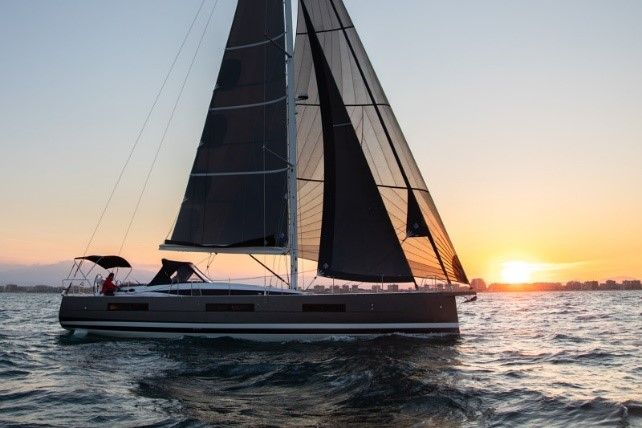
\includegraphics[width=0.45\textwidth]{test_1.jpg}}			  % 子图1的图片宽度 不能空行
    \subfigure[Subfigure Name2(right)]{				% 图片2,其中width代表图片宽度,可以调整
    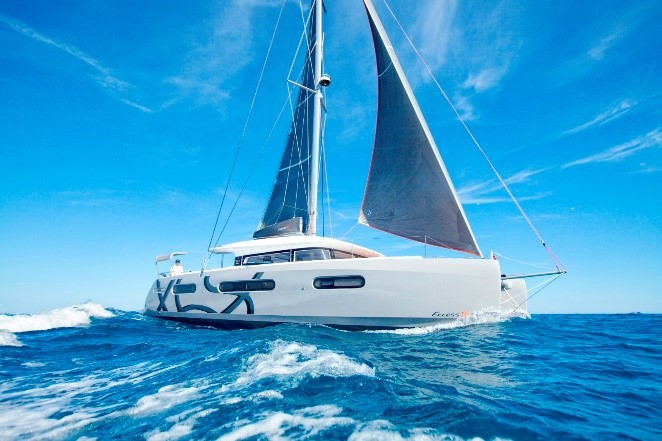
\includegraphics[width=0.45\textwidth]{test_2.jpg}} %注意此处的文件格式为.jpg
	\caption{Figure Name} % 图片标题 
\end{figure}
\vspace{-1cm} %下文向下空-1cm
\subsection{Restatement of the Problem}

%----------------------------------无序列表的排版与语法
\begin{itemize}
    \setlength{\parsep}{0ex} %段落间距
    \setlength{\topsep}{2ex} %列表到上下文的垂直距离
    \setlength{\itemsep}{1ex} %条目间距
    \item Problem 1: 
    \item Problem 2:
    \item Problem 3: 
    \item Problem 4\&5: 
\end{itemize}

%---------------------------------大图的排版与语法
\begin{figure}[H]  %h此处,t页顶,b页底,p独立一页,浮动体出现的位置
    \centering  %图表居中
    
\includegraphics[width=.80\textwidth]{cat.jpeg} %图片的名称或者路径之中有空格会出问题 
    \caption{Flow Chart of this Paper's Research} % 图片标题 
\end{figure}
\vspace{-1cm}

%--------------------------------假设部分较复杂的无序列表
\section{Assumptions and Explanations}
Considering ...
\begin{enumerate}[\bfseries \textit{Assumption} 1:]
	\item \textbf{We assume that ...}\\
	\textbf{\textit{Explanation:}}...
	\item \textbf{We assume that ...}\\
	\textbf{\textit{Explanation:}}...
	\item \textbf{We assume ...}\\
	\textbf{\textit{Explanation:}}...
\end{enumerate}

\section{Notations}
Some important mathematical notations used in this paper are listed in \Cref{tb:notations}. 
%上部对于table的处理使用了交叉引用可以实时更改序号
\begin{table}[H]
\begin{center}
\caption{Notations used in this paper}\label{tb:notations}
\begin{tabular}{c c c}
\toprule[2pt] %三线表顶端线宽度
\multicolumn{1}{m{1.5cm}}{\centering \textbf{Symbol}} %开始写表内容捏,其中{m{xxcm}}表示该列宽度
&\multicolumn{1}{m{12.5cm}}{\centering\textbf{Description} }
&\multicolumn{1}{m{1cm}}{\centering \textbf{Units}}\\
\midrule
$\lambda_i$& Meaning of the symbol&/ \\
$y_i$& Meaning of the symbol&/\\
$a_i$& Meaning of the symbol&/\\
$\Delta R$&Meaning of the symbol&/ \\
$R^*$ &Meaning of the symbol &/\\
\bottomrule[2pt]
\end{tabular}

\begin{tablenotes}%等等,表格还有些说明!
        \footnotesize
        \item[*] *There are some variables that are not listed here and will be discussed in detail in each section. %此处加入注释*信息
\end{tablenotes}
\end{center}
\end{table}
\vspace{-1.2cm}%在\end{table}下加一行\vspace{-1cm} 其中-1的作用是缩短与下方文字距离的 切记!必须是负数

\section{Model Preparation}
\subsection{Data Overview}
For a large amount of data, it is necessary to process and clean the data before building the model. So we first use the ismissing function to find the missing value and get the missing value in \Cref{tb:missing_data}:
\begin{table}[H]%浮动体的htbp可以强制在原位显示,改参数为H
  \begin{center}
  \fontsize{12pt}{13.8}
  \caption{Missing Data in Given Data} \label{tb:missing_data}
  \resizebox{\textwidth}{!}
  {\begin{tabular}{||l|l|c c c c|r|r||} %此处设置了不同类型的参数及线供参考
  \toprule[2pt]
  \multicolumn{1}{m{3cm}}{\centering \textbf{Missing1}} %大型表格需要好好斟酌每一列的宽度捏
  &\multicolumn{1}{m{2cm}}{\centering \textbf{Missing2}}
  &\multicolumn{1}{m{2cm}}{\centering \textbf{Missing3}}
  &\multicolumn{1}{m{2cm}}{\centering \textbf{Missing4}}
  &\multicolumn{1}{m{2cm}}{\centering \textbf{Missing5}}
  &\multicolumn{1}{m{2cm}}{\centering \textbf{Missing6}}
  &\multicolumn{1}{m{2cm}}{\centering \textbf{Missing7}}
  &\multicolumn{1}{m{2cm}}{\centering \textbf{Missing8}}
  \\ %m后面是列宽
  \midrule
  \multirow{3}*{\makecell[c]{Looooog\\Word}}%合并行操作,同时进行了合并行内的换行,{}内是合并的行数
  &A&B&C&D&-&E&F \\
  ~ &A&B&C&D&-&E&F   \\
  ~ &A&B&C&D&-&E&F \\ 
  Multicolumn&\multicolumn{7}{c}{These columns share common features} \\%合并列操作,{}内是合并的列数
  \bottomrule[2pt]
  \end{tabular}}
  \end{center}
\end{table}
\vspace{-1cm}

\subsubsection{Data Collection}
And other data sources are shown in \Cref{tb:data_source}.

\begin{table}[H]
    \begin{center}
    \caption{Data and Database Websites}\label{tb:data_source}
    \resizebox{\textwidth}{!}
    {\begin{tabular}{c c}
    \toprule[2pt]
    \multicolumn{1}{m{6.5cm}}{\centering \textbf{Database Names}}
    &\multicolumn{1}{m{10cm}}{\centering \textbf{Database Websites} }\\ %m后面是列宽
    \midrule
    GDP of Each Country& https://ourworldindata.org/ \\
    GDP of Some European Countries & https://data.worldbank.org/ \\
    \multirow{2}*{Partial Sailing Parameters}& https://www.sailboat-cruising.com/\\ 
    ~& https://sailboatdata.com/ \\
    \bottomrule[2pt]
    \end{tabular}}
    \end{center}
\end{table}
\vspace{-1cm}

\subsubsection{Data Screening}
According to the data given, we...
\begin{figure}[htbp]
    \centering    
    \subfigure[Cute Cat(left)]{									
    
\includegraphics[width=0.45\textwidth]{catsquare.jpeg}}			 
    \subfigure[Cute Cat(right)]{				
    
\includegraphics[width=0.45\textwidth]{catsquare.jpeg}} %此时两张图片的大小不一样就需要改width参数
	\caption{Data Screening}  
\end{figure}
\vspace{-1cm}

This is a double-table.

\begin{table}[H] %浮动体的htbp可以强制在原位显示,改参数为H
    \begin{center}
    \caption{Partial Monohull and Catamaran data}
    \resizebox{\textwidth}{!}
    {\begin{tabular}{c c c c c c}
    \toprule[2pt]
    \multicolumn{1}{m{4cm}}{\centering \textbf{AA}}
    &\multicolumn{1}{m{2cm}}{\centering \textbf{BB$/m$}}
    &\multicolumn{1}{m{2cm}}{\centering \textbf{CC/m$^3$}}
    &\multicolumn{1}{m{2cm}}{\centering \textbf{DD\\/m$^3$}}%此处如果DD过长可以使用\\换行
    &\multicolumn{1}{m{2cm}}{\centering \textbf{EE/m$^2$}}
    &\multicolumn{1}{m{4cm}}{\centering \textbf{FF}}
    \\ %m后面是列宽
    \midrule
    A&B&C&D&E&F \\
    A&B&C&D&E&F\\
    \bottomrule[2pt]
    \toprule[2pt]
    \multicolumn{1}{m{4cm}}{\centering \textbf{AA}}
    &\multicolumn{1}{m{2cm}}{\centering \textbf{BB$/m$}}
    &\multicolumn{1}{m{2cm}}{\centering \textbf{CC/m$^3$}}
    &\multicolumn{1}{m{2cm}}{\centering \textbf{DD\\/m$^3$}}%此处如果DD过长可以使用\\换行
    &\multicolumn{1}{m{2cm}}{\centering \textbf{EE/m$^2$}}
    &\multicolumn{1}{m{4cm}}{\centering \textbf{FF}}
    \\ %m后面是列宽
    \midrule
    A&B&C&D&E&F \\
    A&B&C&D&E&F\\
    \bottomrule[2pt]
    \end{tabular}}
    \end{center}
  \end{table}

\section{Fusion Model based on RF, BP and CNN Algorithm}
\subsection{The Transformation and Dimensionality Reduction of Sailing Price Index}
Since one of the above Hull materials is a qualitative index, it is now converted into a quantitative index for subsequent calculation through the following rules.

\begin{table}[htbp]
    \begin{center}
    \caption{Rules for Quantitative Conversion of Hull Material Index}
    \resizebox{\textwidth}{!}
    {\begin{tabular}{c c c c}
    \toprule[2pt]
    Hull Materials&Values&Hull Materials&Values\\ %可以看情况不使用\multicolumn语法
    \midrule
    Glass Reinforced Plastic& 1 &Glass Fibre                     & 3 \\
    Carbon Fiber            & 2 &Glassy CarbonComposite Material & 4 \\
    \bottomrule[2pt]
    \end{tabular}}
    \end{center}
\end{table}

In addition, we will be catamaran as a 0-1 variable, plus hull length and factory year a total of 12 quantitative indicators. The principal component analysis method is selected for dimensionality reduction.

Principal component analysis (PCA) is a statistical method for dimensionality reduc-tion. Through orthogonal transformation, the original random vector with component corre-lation is transformed into a new random vector with component uncorrelation, and the orig-inal variable is recombined into a group of several new comprehensive variables which are independent of each other. 

\begin{enumerate}[\bfseries 1.]
    \setlength{\parsep}{0ex} %段落间距
    \setlength{\topsep}{0ex} %列表到上下文的垂直距离
    \setlength{\itemsep}{0ex} %条目间距
    \item The covariance matrix of 12 indexes can be obtained after centralization and mean removal.
    \begin{align}
        C=\left[ \begin{matrix}
	    Cov\left( x_1,x_1 \right)&		Cov\left( x_1,x_2 \right)\\
	    Cov\left( x_2,x_1 \right)&		Cov\left( x_2,x_2 \right)\\
        \end{matrix} \right] ,\ \text{where\ }Cov\left( x_2,x_1 \right) =\frac{\sum_{i=1}^M{\left( x_{1}^{i}-\overline{x_1} \right) ^2}}{M-1}
    \end{align}
    In the above matrix, the diagonal is the variance of index and, and the non-diagonal is the covariance.
   
    \item By calculating the eigenvalues and eigenvectors of the covariance matrix, we can project the original features onto the selected eigenvectors and obtain the new K-dimensional features after dimensionality reduction.
    \begin{align}
      \left[ \begin{array}{c}
	    y_{1}^{i}\\
	    y_{2}^{i}\\
	    \vdots\\
	    y_{k}^{i}\\
        \end{array} \right] =\left[ \begin{matrix}
	    u_{1}^{T}&		\cdots&		\left( x_{1}^{i},x_{2}^{i},x_{3}^{i},\cdots ,x_{N}^{i} \right) ^T\\
	    u_{2}^{T}&		\cdots&		\left( x_{1}^{i},x_{2}^{i},x_{3}^{i}\cdots ,x_{N}^{i} \right) ^T\\
	    \vdots   &		\cdots&		\vdots\\
	    u_{k}^{T}&		\cdots&		\left( x_{1}^{i},x_{2}^{i},x_{3}^{i},\cdots ,x_{N}^{i} \right) ^T\\
        \end{matrix} \right] 
    \end{align}    
    The dimensionality reduction process is actually to project the original eigenvalue A $\left( x_{1}^{i},x_{2}^{i},x_{3}^{i},\cdots ,x_{N}^{i} \right) ^T$ of each sample into the new eigenvalue $\left( y_{1}^{i},y_{2}^{i},y_{3}^{i},\cdots ,y_{N}^{i} \right) ^T$B, and the above formula is the calculation formula of the new feature.
    \item Through the above treatment, we can use the afternoon formula to calculate the contribution rate and cumulative contribution rate of each principal component;
    \begin{align}
        Con=\frac{\lambda _i}{\sum_{k=1}^p{\lambda _k}},\ \left( i=1,2,\cdots ,p \right) \\
        Con^*=\frac{\sum_{k=1}^i{\lambda _k}}{\sum_{k=1}^p{\lambda _k}},\ \left( i=1,2,\cdots ,p \right) 
    \end{align}
\end{enumerate}

We take the eigenvalue of the cumulative contribution rate between 80\% and 90\%. Where $\lambda _1,\lambda _2,\lambda _3,\cdots ,\lambda _i$ is the corresponding 1 to n principal components.
After the above calculation, we can get the results of principal component analysis as shown in the table below.

\begin{table}[htbp]
    \begin{center}
    \caption{Each Principal Component and its Cumulative Contribution Rate}
    \resizebox{\textwidth}{!}
    {\begin{tabular}{c c c c c c}
    \toprule[2pt] %在表内换行时使用\makecell[c]{A//B}的语法
    \centering \textbf{\makecell[c]{Principal\\Component}}  &\centering \textbf{\makecell[c]{Characteristic\\Root}}   &\centering \textbf{ \makecell[c]{Cumulative \\Contribution Rate}} 
    & \centering \textbf{\makecell[c]{Principal\\Component}} & \centering \textbf{\makecell[c]{Characteristic\\Root}}  &\textbf{\makecell[c]{Cumulative \\Contribution Rate}}\\
    \midrule
    $\lambda_1$& 4.5138 &37.61\% &$\lambda_7$   & 0.4898 &88.87 \%\\
    $\lambda_2$& 1.7215 &51.96\% &$\lambda_8$   & 0.4001 &92.20 \%\\
    $\lambda_3$& 1.2331 &62.24\% &$\lambda_9$   & 0.3735 &95.32 \%\\
    $\lambda_4$& 1,0683 &71.14\% &$\lambda_{10}$& 0.3075 &97.88 \%\\
    $\lambda_5$& 0.9123 &78.74\% &$\lambda_{11}$& 0.1543 &99.16 \%\\
    $\lambda_6$& 0.7256 &84.79\% &$\lambda_{12}$& 0.1002 &100.00\%\\
    \bottomrule[2pt]
    \end{tabular}}
    \end{center}
\end{table}
\vspace{-0.5cm}
The red marks in the table above represent the principal components we have selected. It can be seen that the cumulative contribution rate of the 6 principal components is close to 85\%, so it is very reasonable to choose these as the principal components.

The eigenvectors of some principal components are shown in the following table.




\begin{table}[H] 
    \begin{center}
    \caption{Partial Principal Component Eigenvectors}
    \resizebox{\textwidth}{!}
    {\begin{tabular}{c c c c c c c}
    \toprule[2pt]
    \textbf{/}&\textbf{Year}&\textbf{Beam length/m}&\textbf{Draft/m$^3$}&\textbf{Displacement/m$^3$}&\textbf{Sail area/m$^2$}&\textbf{Hull materials}\\ %m后面是列宽
    \midrule
    $\lambda_1$&7.2&1.15&11800&116&Carbon fiber&-0.0165 \\
    $\lambda_6$&6.7&1.95&18000&163&Aluminium alloy&0.3338\\
   % \hline\hline
    \bottomrule[2pt]
    \toprule[2pt]
    \textbf{/}&\textbf{\makecell[c]{Engine\\hours/h}}&\textbf{\makecell[c]{Sleeping\\capacity/person} }&\textbf{Head-room/m}&\textbf{GDP/ Trillion\$}&\textbf{Length/ft}&\textbf{Catamarans?}\\ %m后面是列宽
    \midrule
    $\lambda_1$&7.2&1.15&11800&116&Carbon fiber&-0.0165 \\
    $\lambda_6$&6.7&1.95&18000&163&Aluminium alloy&0.3338\\
   % \hline\hline
    \bottomrule[2pt]


    \end{tabular}}
    \end{center}
\end{table}
\vspace{-1cm}
Index dimension reduction can remove redundancy and noise features in the data, thus reducing the dimension of the data set, simplifying the complexity of the machine learning model, improving the generalization ability of the model, and avoiding the problem of over-fitting. Therefore, index dimension reduction can improve the efficiency and accuracy of machine learning algorithms on the premise of maintaining the integrity of data information

\vspace{-0.5cm}

\subsection{Price Prediction of RF, BP and CNN Algorithm}
Random forest (RF)[1,2] is an integrated learning method that integrates multiple trees. It has the advantages of high accuracy and can be run on large data sets.

The BP neural network calculates the loss function according to the forward propaga-tion of the input sample. If the error is inconsistent, the error is sent back as the reverse sig-nal, and the weight matrix is constantly modified to finally achieve the prediction effect.

Convolutional neural network (CNN)[3] is a kind of feedforward neural network with depth structure, which is basically divided into three parts: convolutional layer, pooling lay-er and full connection layer. It alleviates the problem of vanishing gradient effectively and reduces the number of parameters to a certain extent.

Sine and cosine algorithm (SCA) is a swarm intelligence optimization algorithm, which has the advantages of few parameters, simple structure and easy implementation. We com-bine it with the above three methods to get the optimized.

We respectively predicted by RF, BP and CNN models, combined with SCA optimiza-tion algorithm to calculate the predicted value of the price and compared it with the original price, as shown in the figure below.

\begin{figure}[H]
    \centering    
    \subfigure[RF Method]{				% 图片1([]内为子图标题)						
    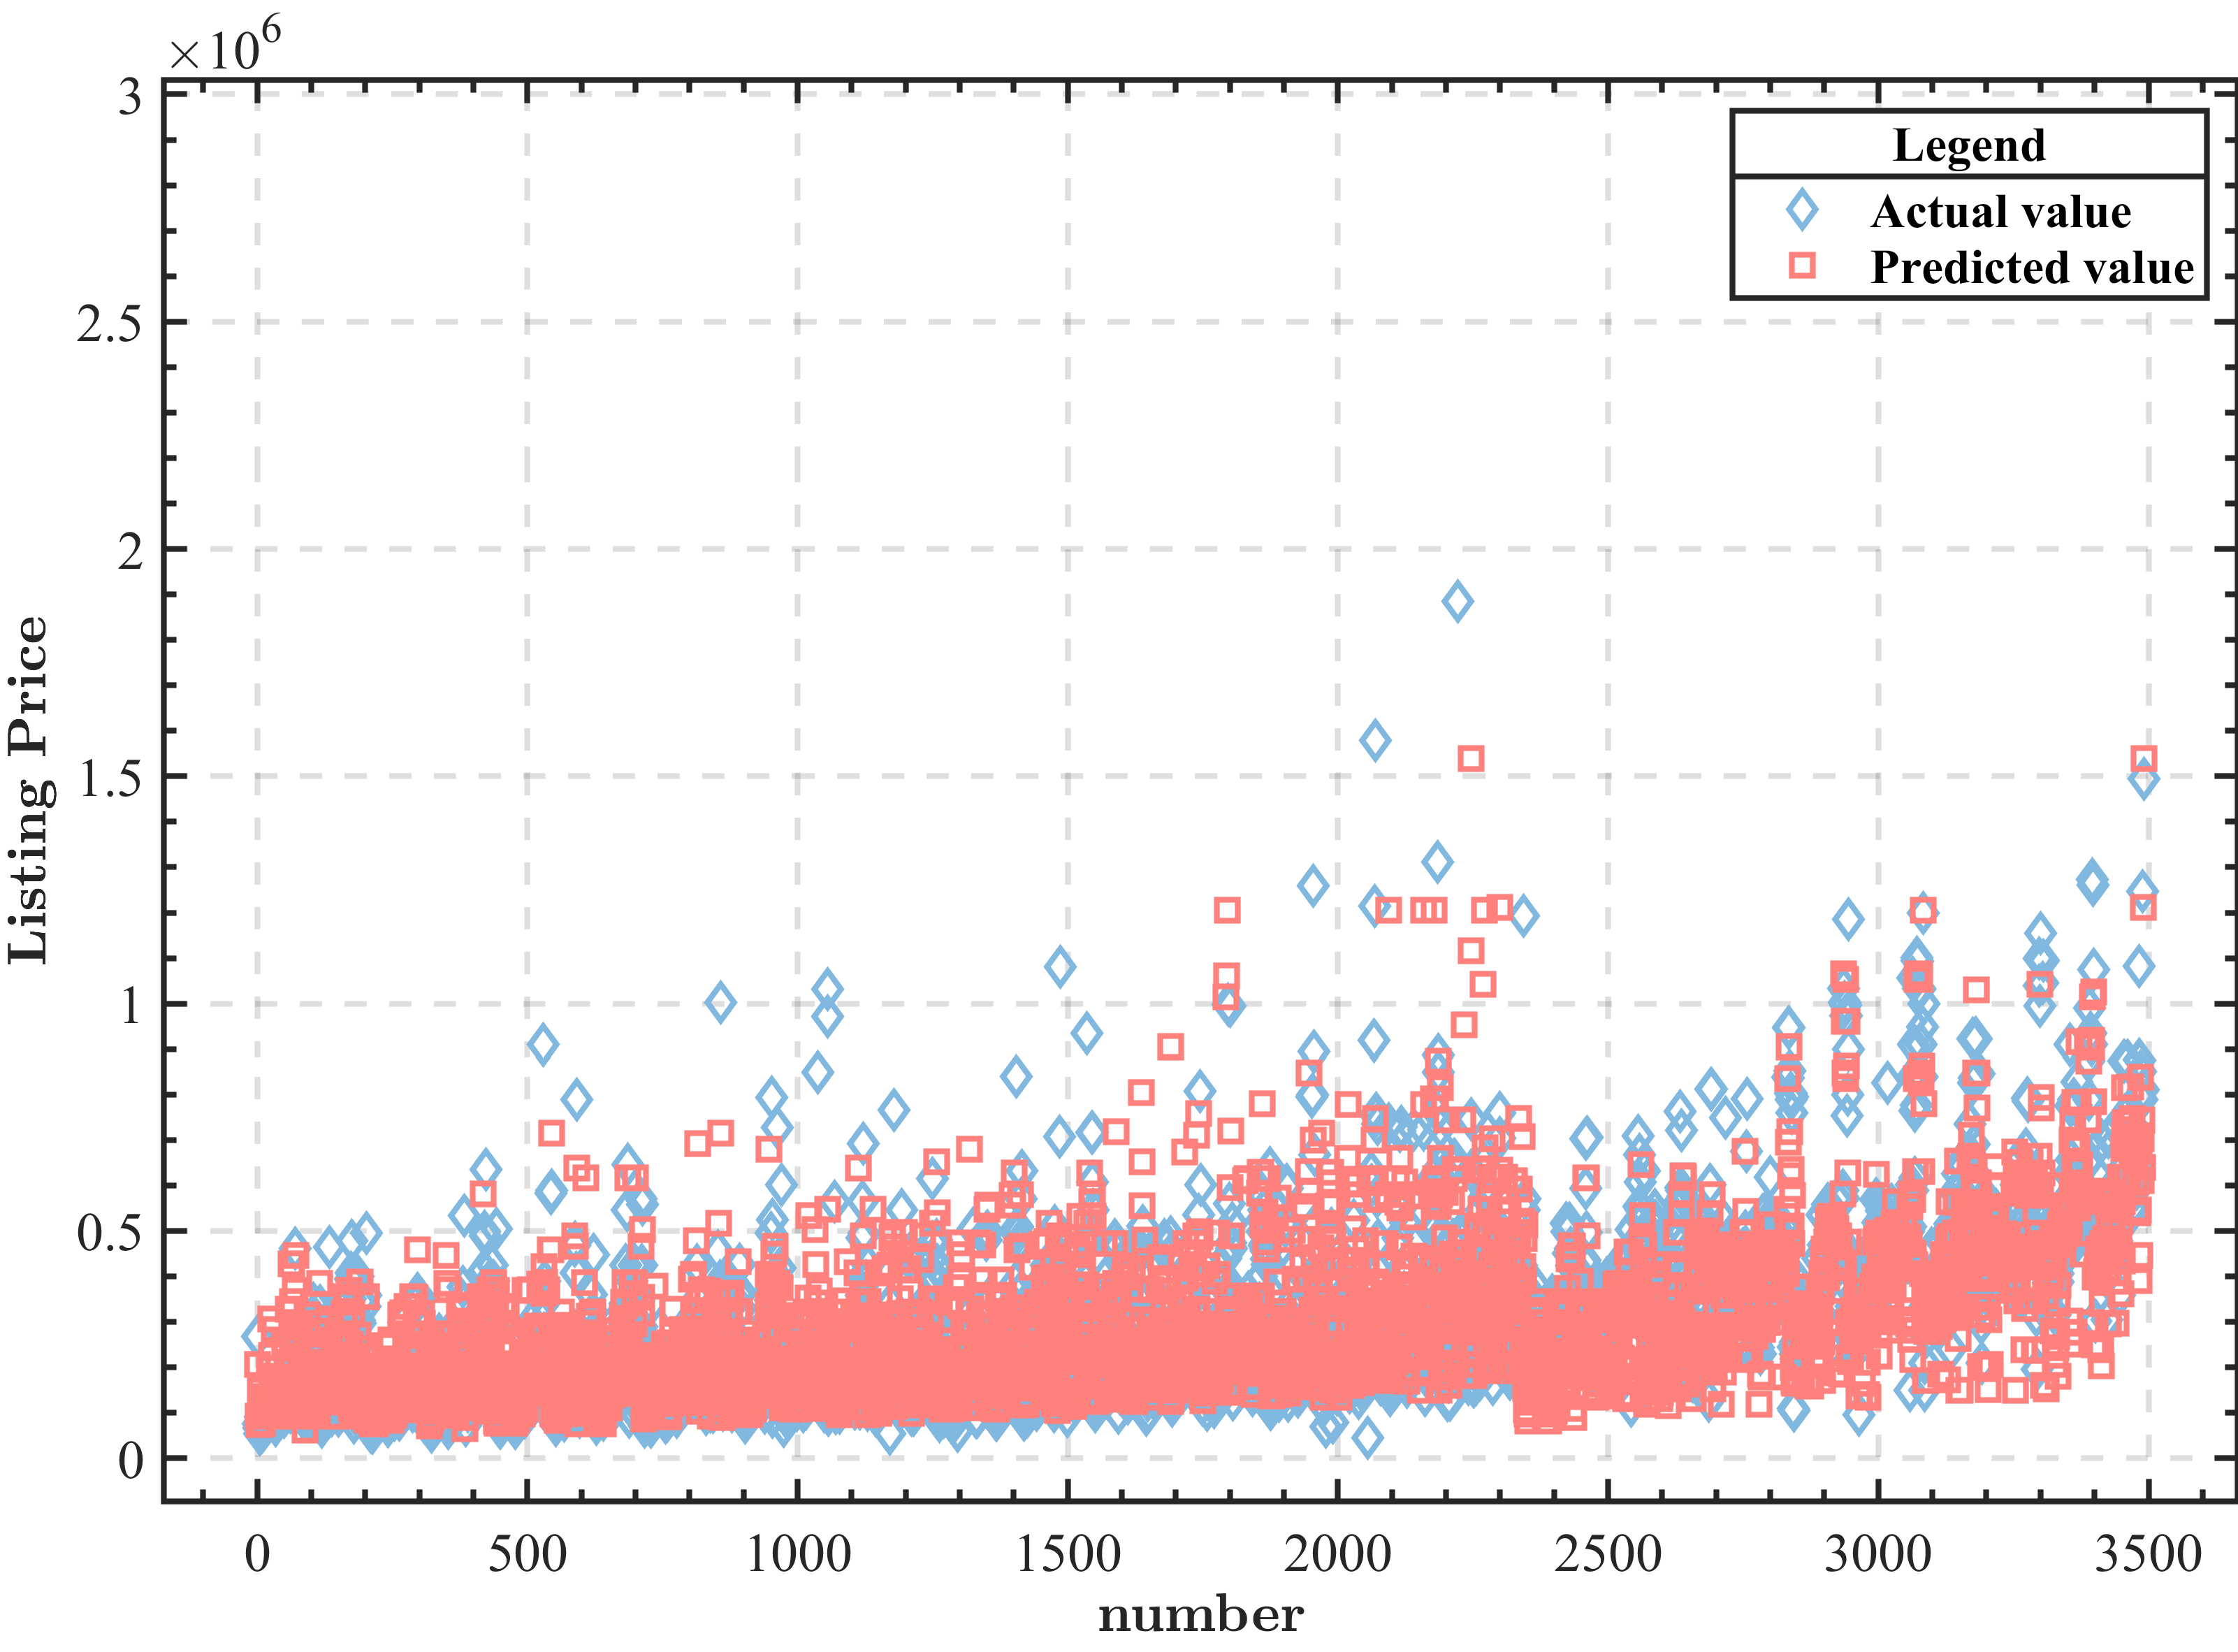
\includegraphics[width=0.31\textwidth]{test_6.png}}			  % 子图1的图片宽度 不能空行
    \subfigure[BP Method]{				% 图片2
    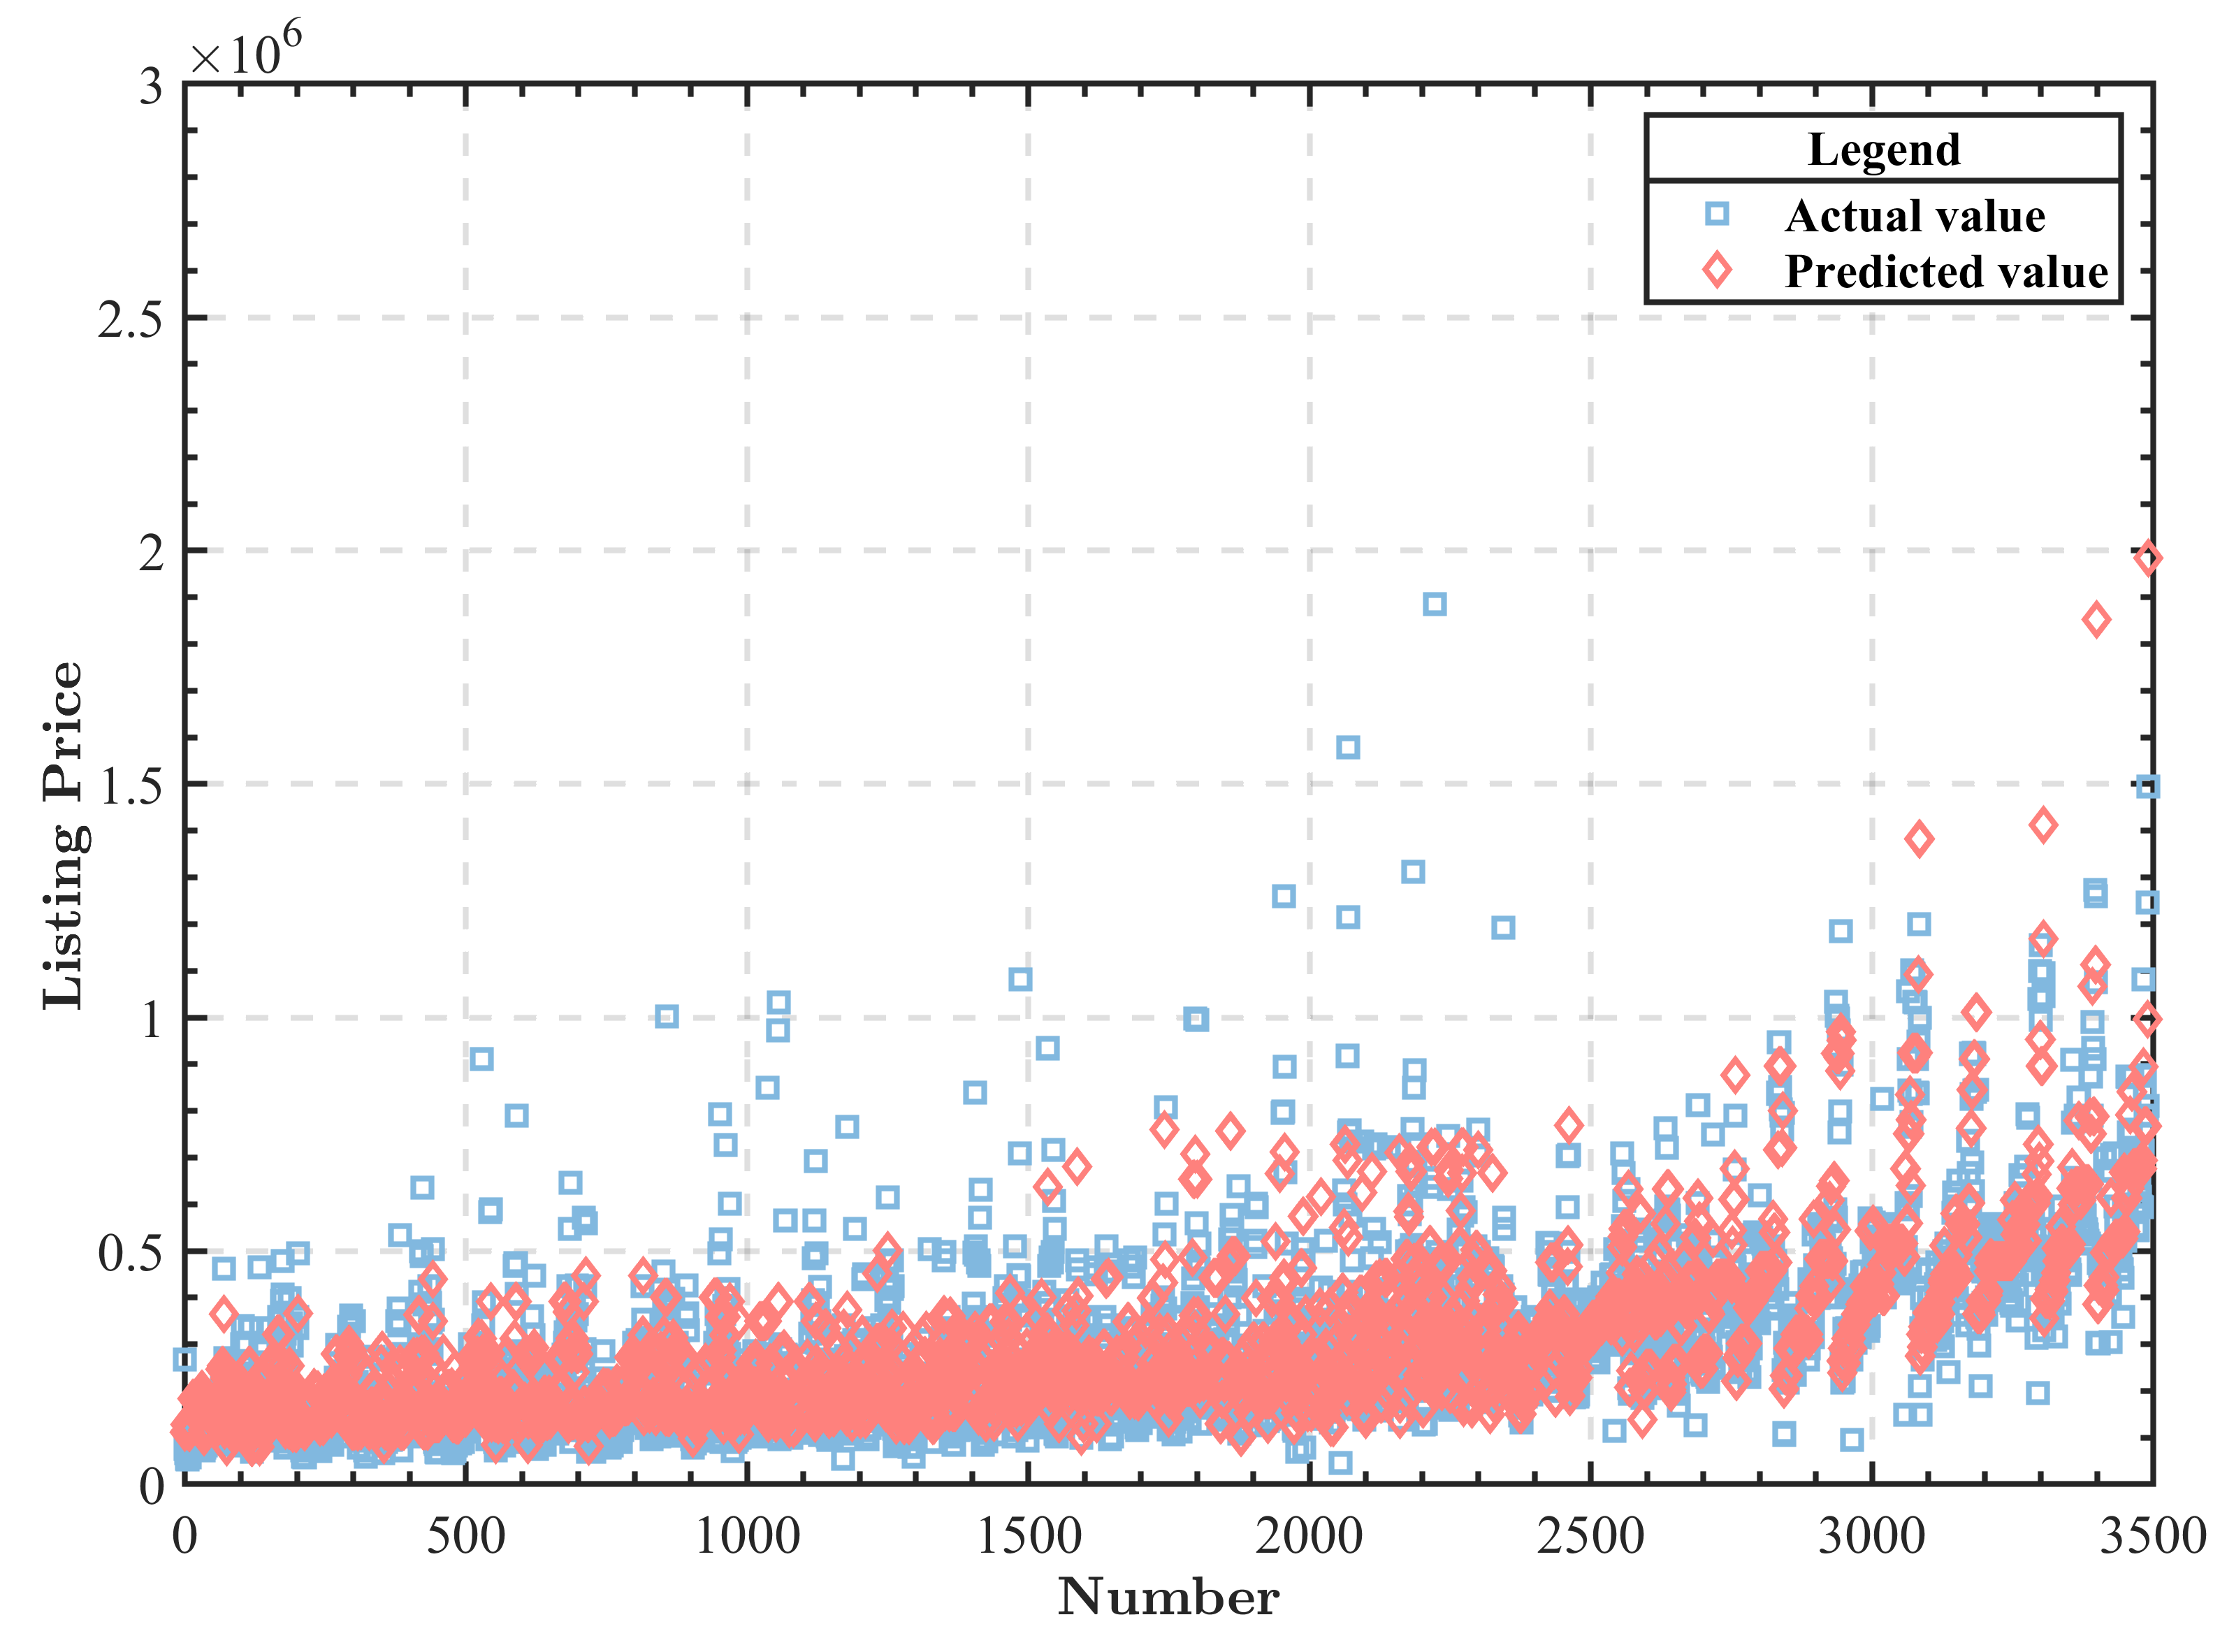
\includegraphics[width=0.31\textwidth]{test_8.png}} 
    \subfigure[CNN Method]{				% 图片2
    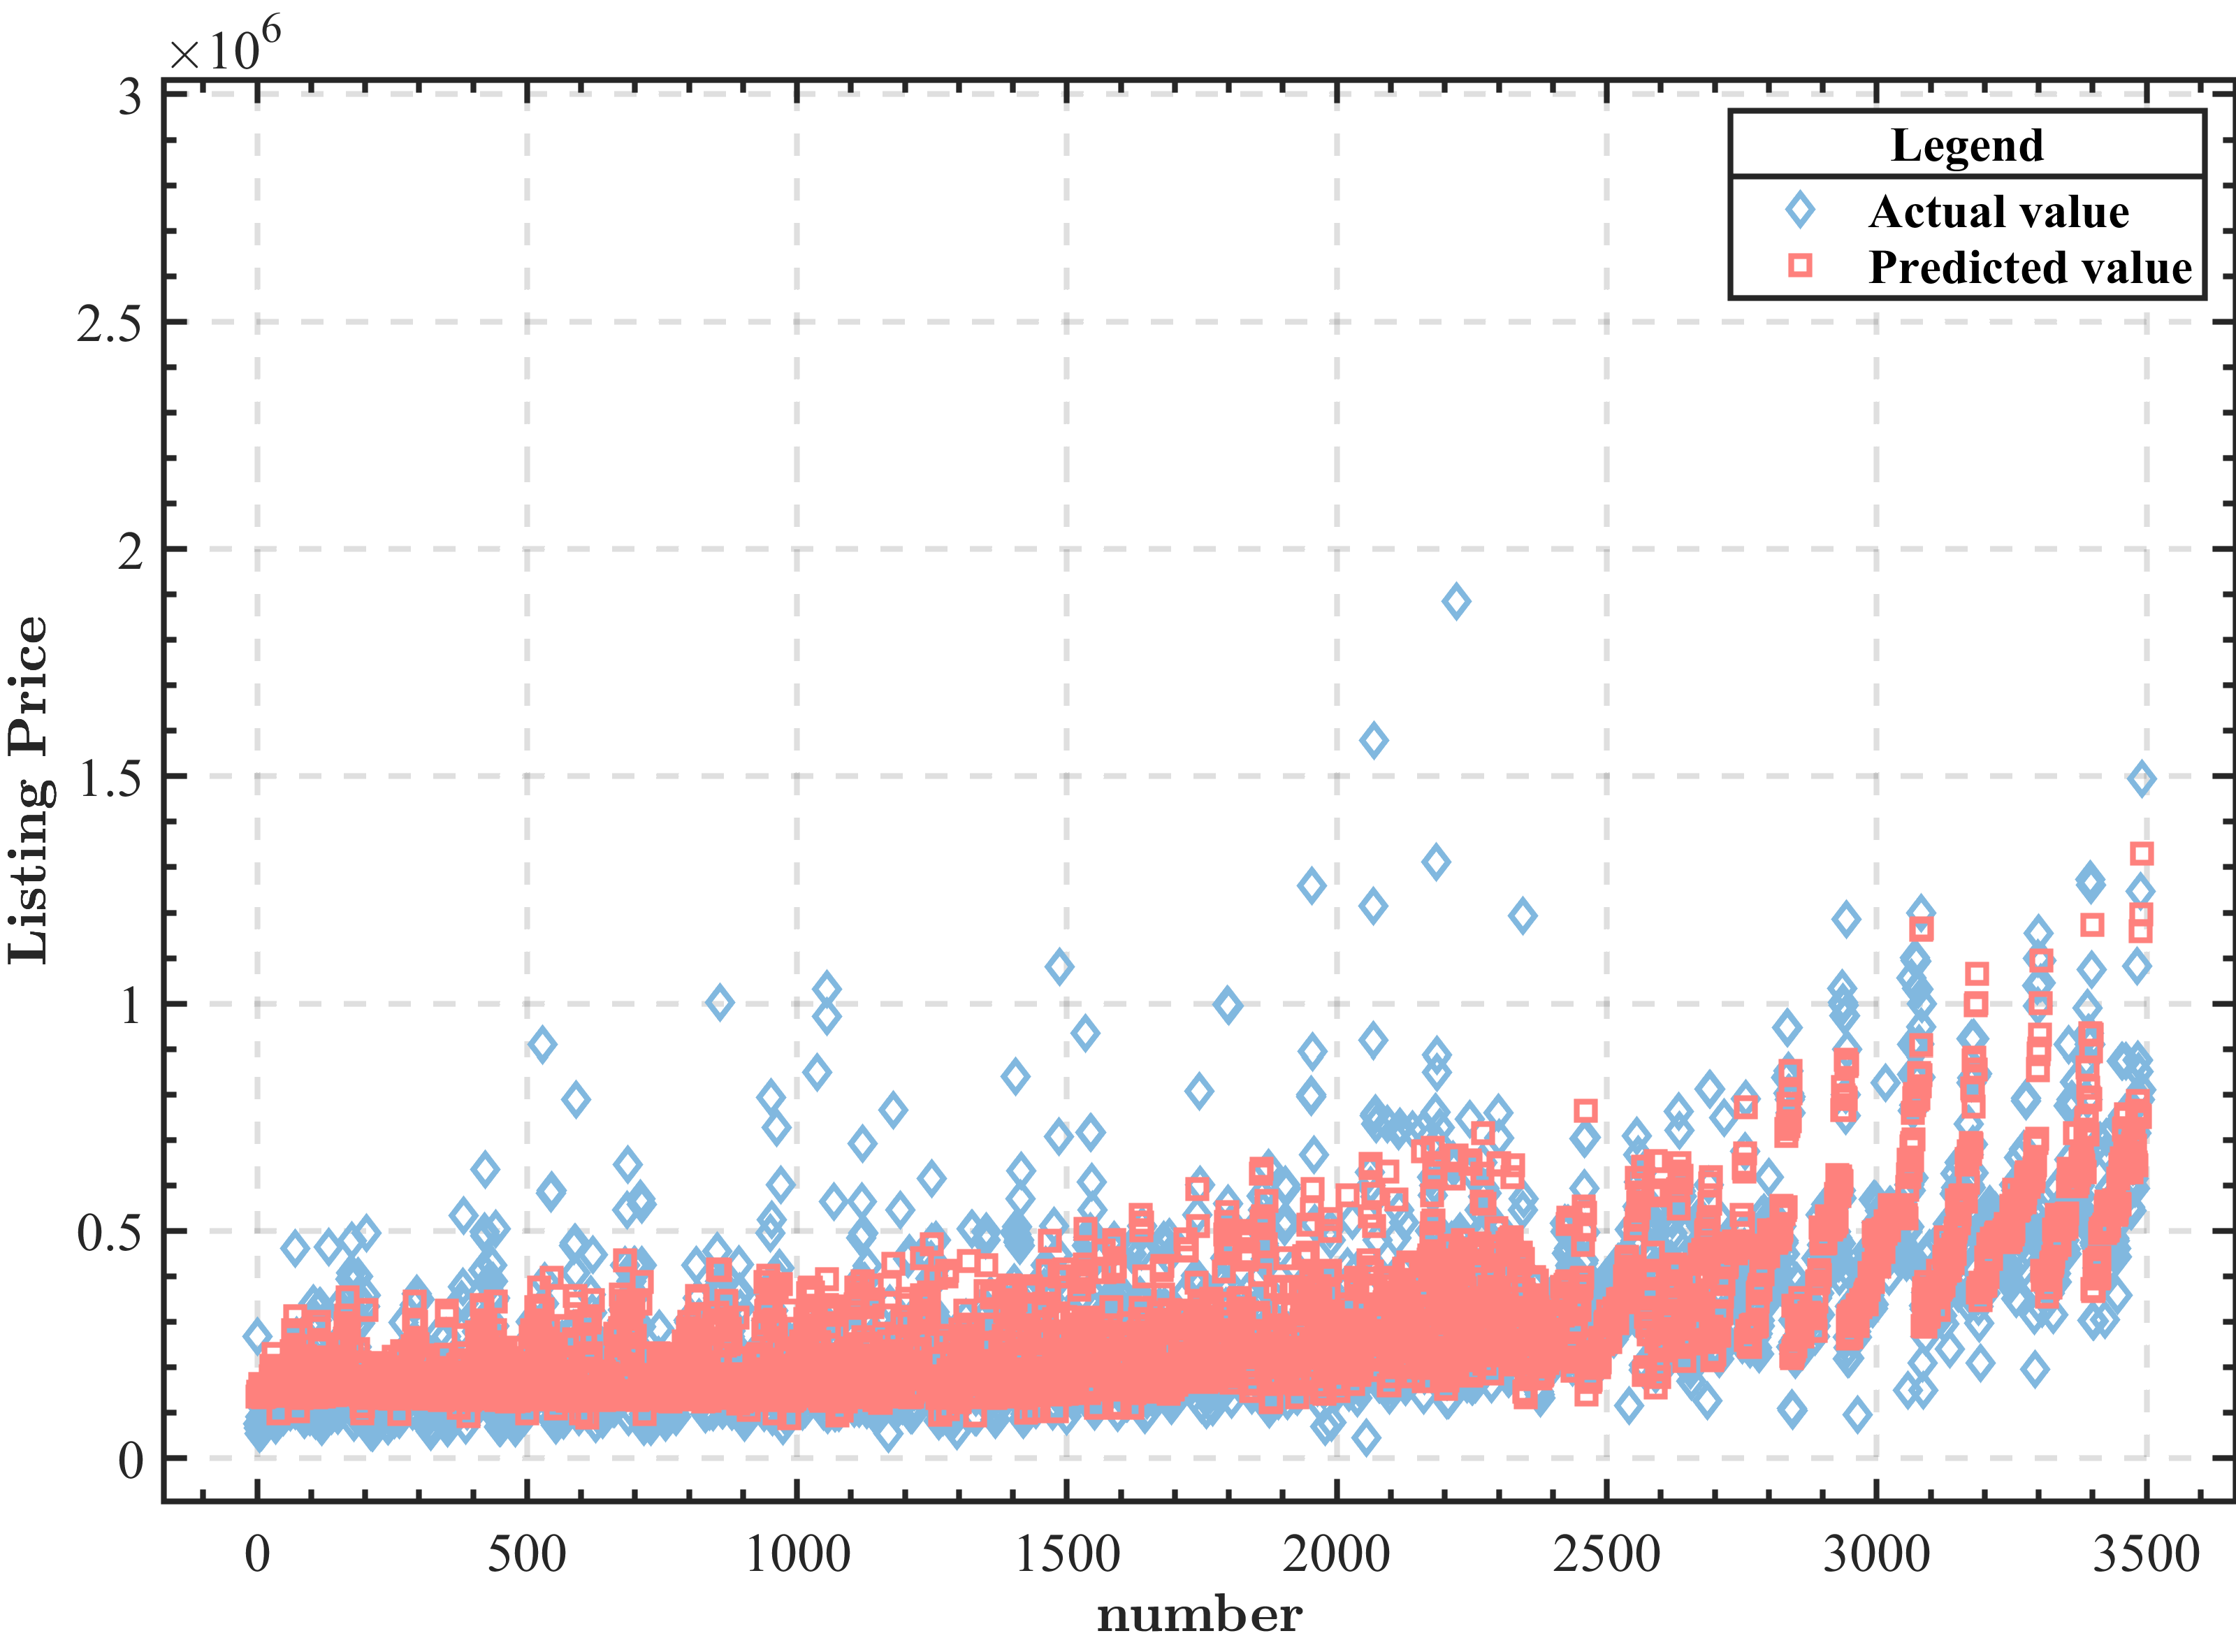
\includegraphics[width=0.31\textwidth]{test_10.png}} 
	\caption{RF, BP, and CNN Predicted Results Compared} % 图片标题 
\end{figure}
\begin{figure}[H]
    \centering  
    \subfigure[MSE of RF Method]{				% 图片1([]内为子图标题)						
    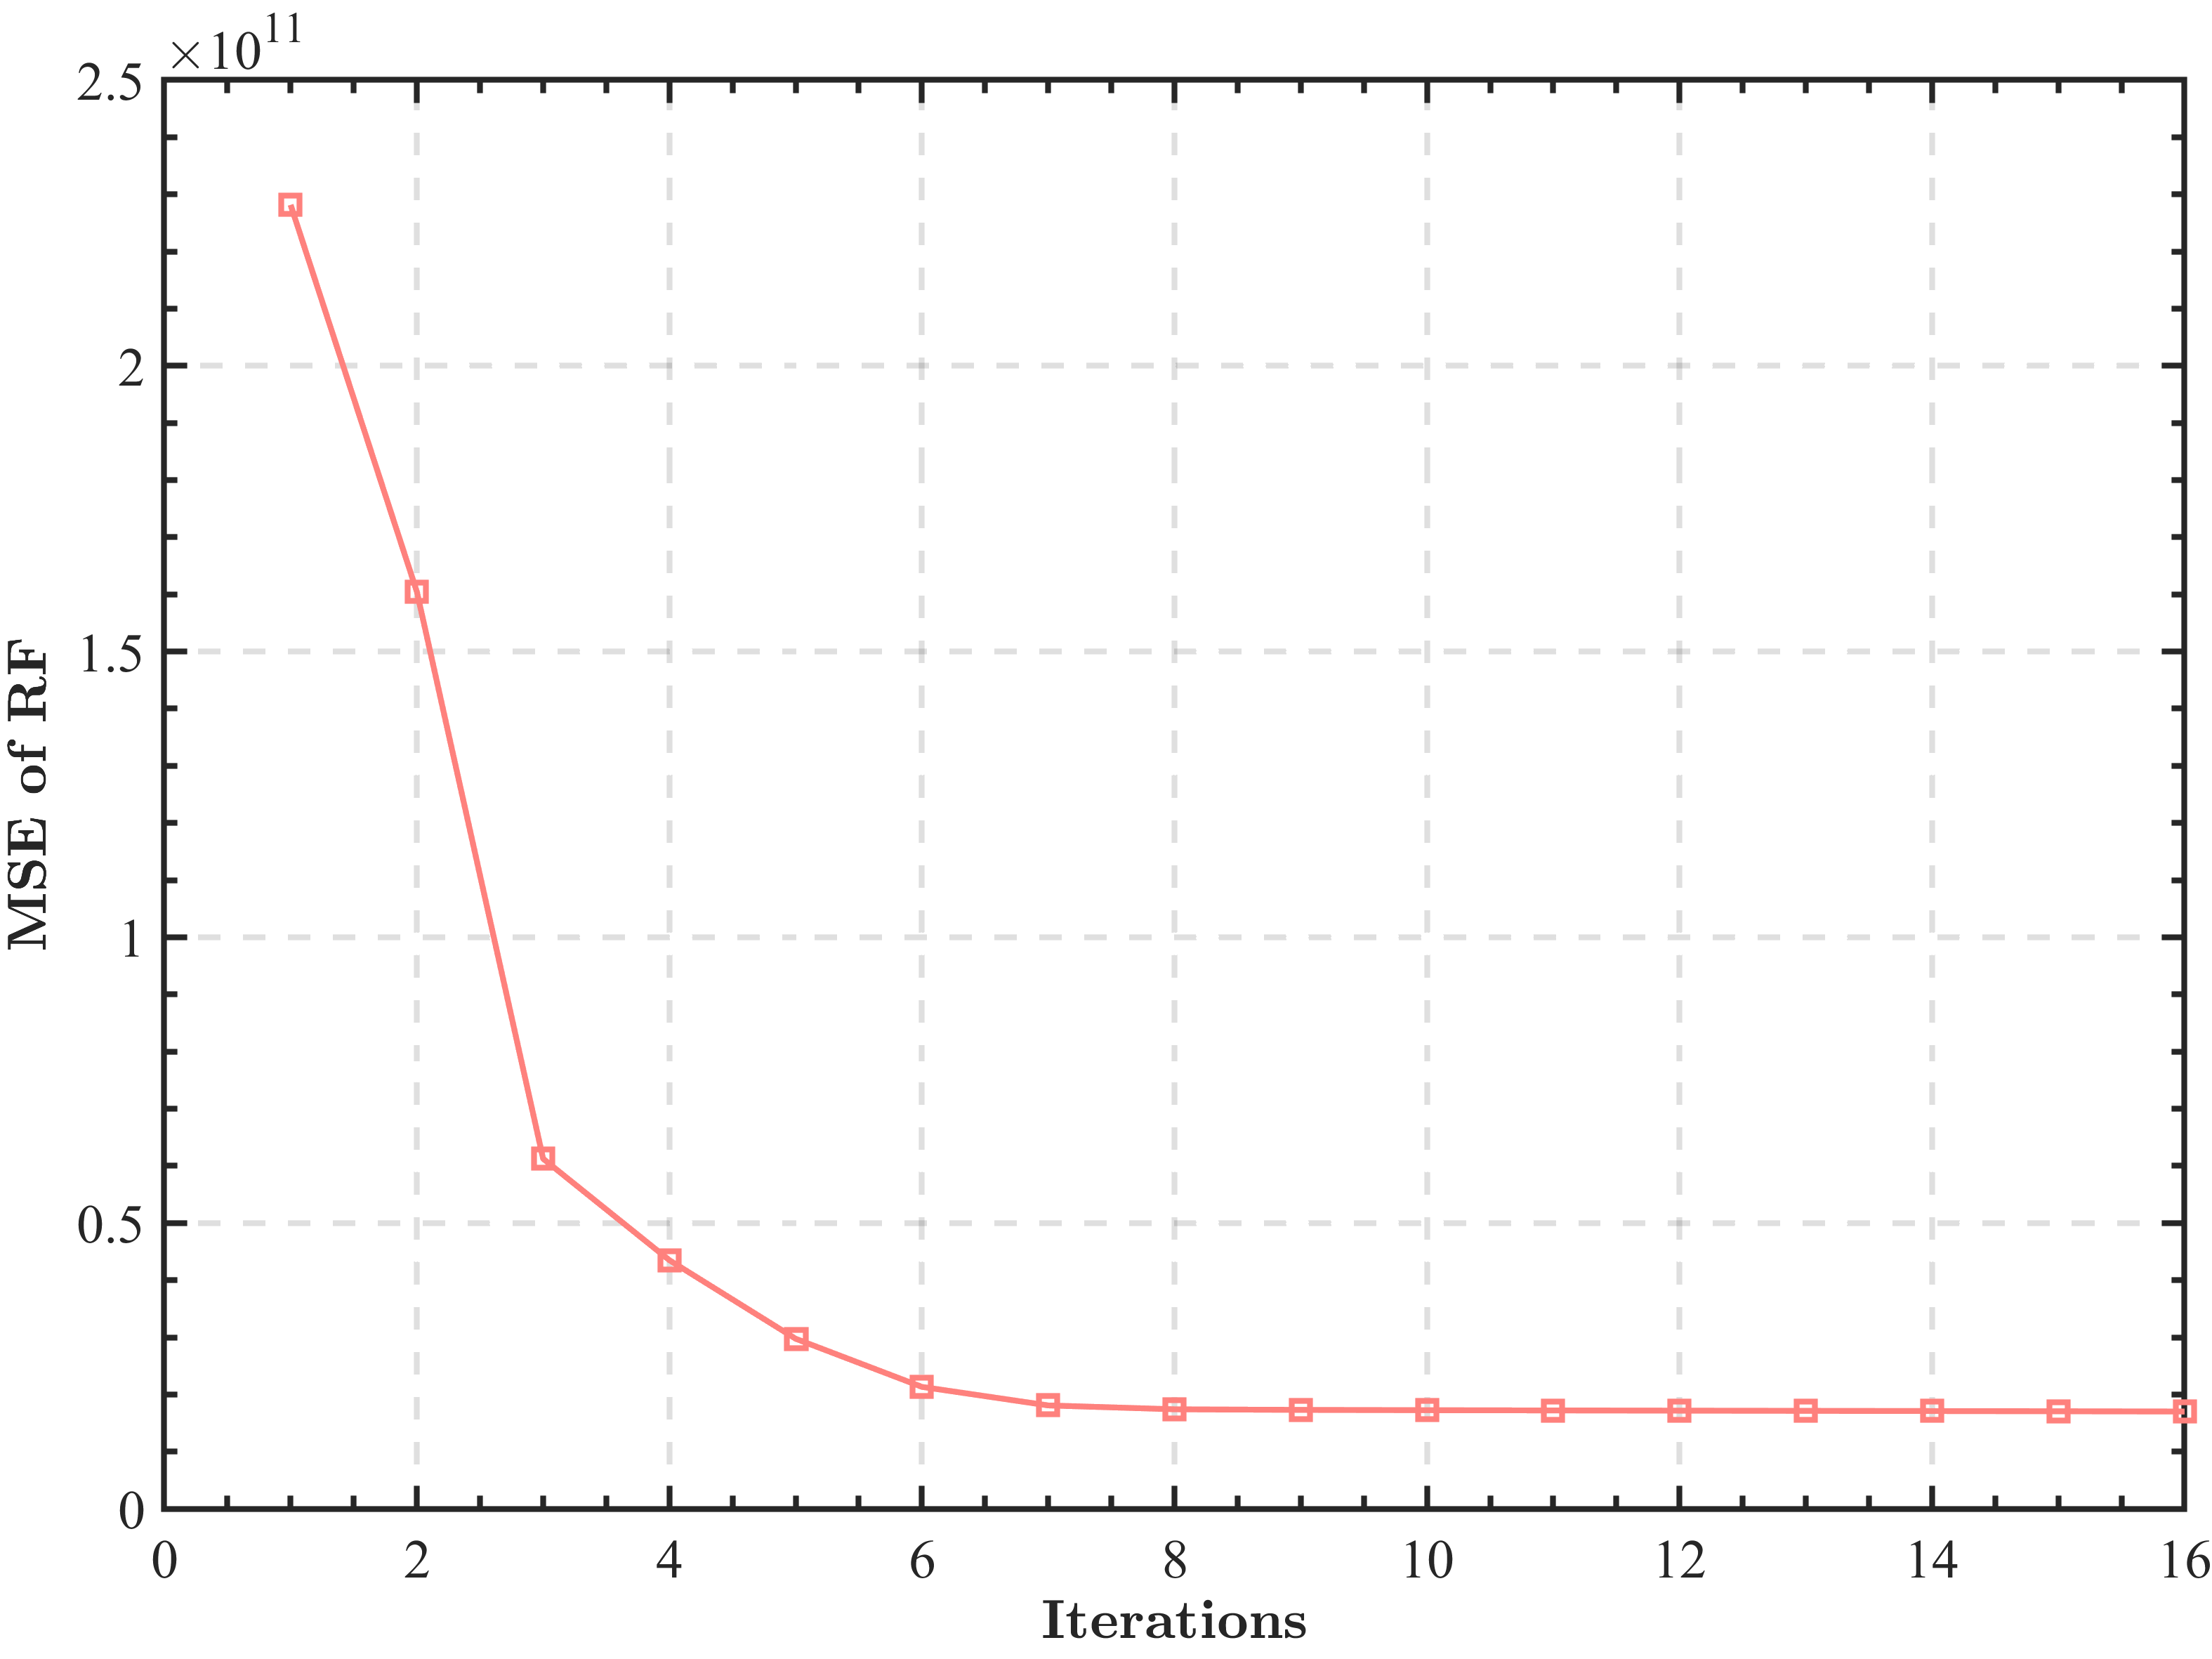
\includegraphics[width=0.30\textwidth]{test_7.png}}			  % 子图1的图片宽度 不能空行
    \subfigure[MSE of BP Method]{				% 图片2
    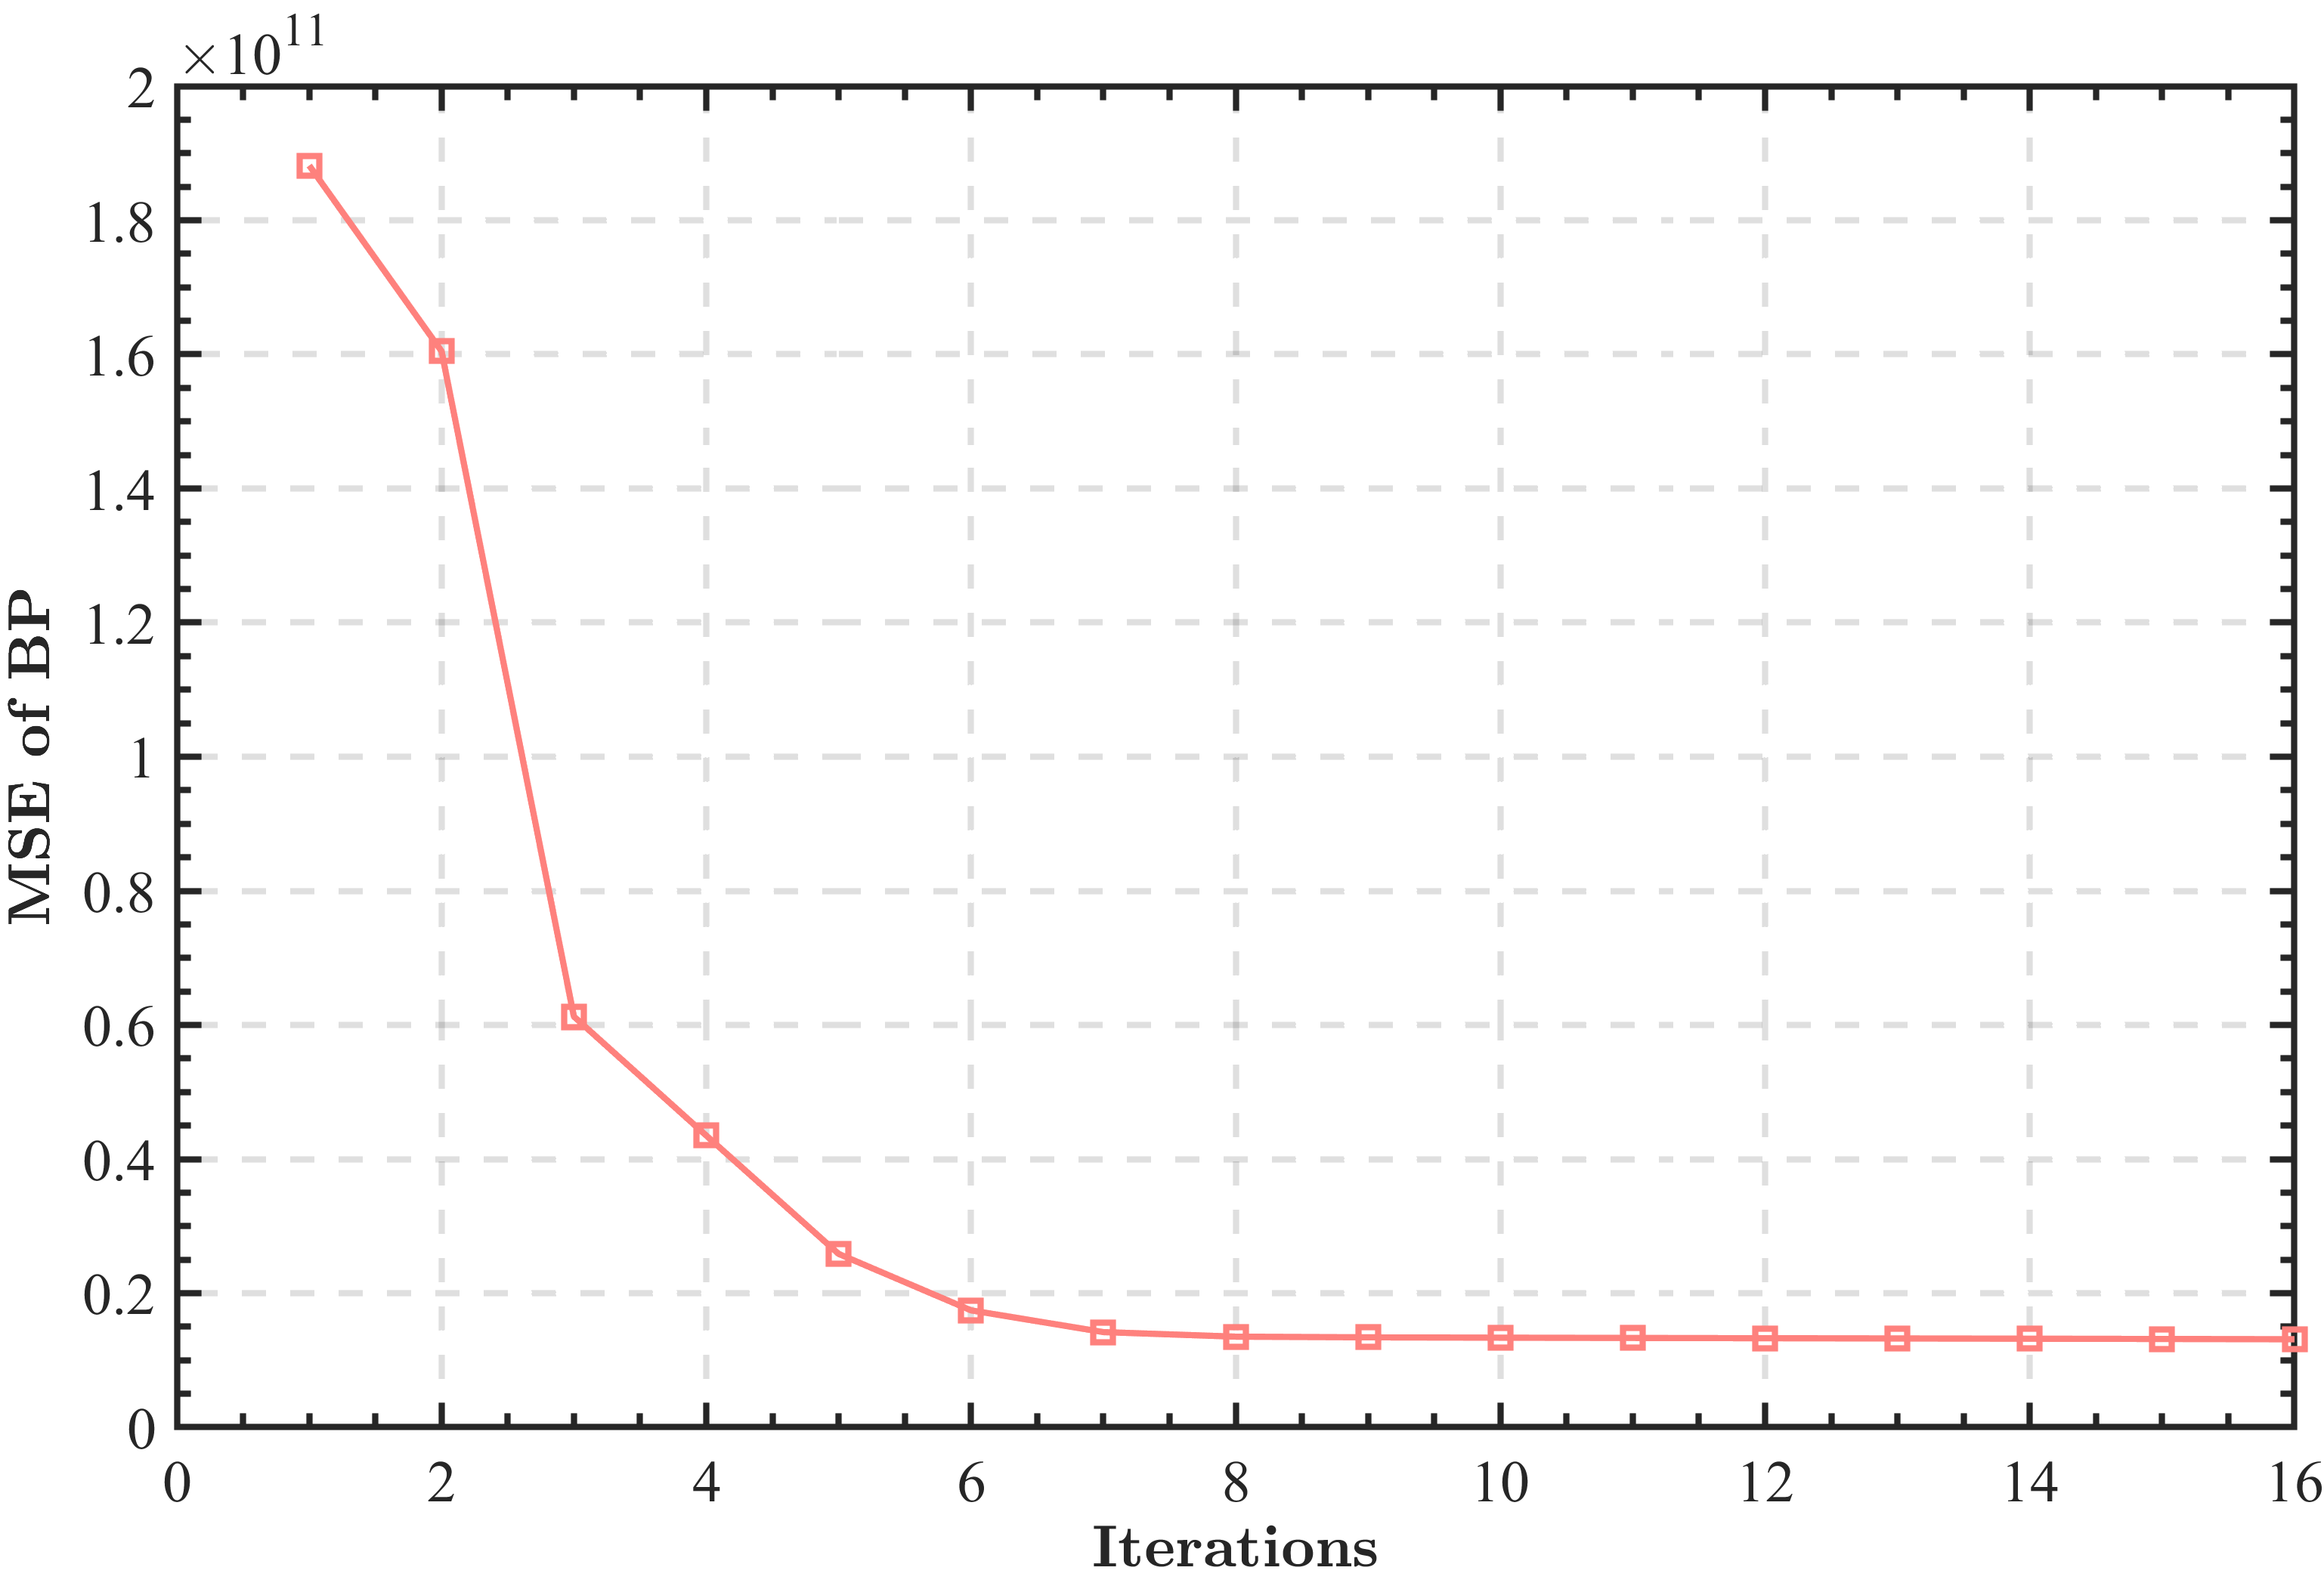
\includegraphics[width=0.33\textwidth]{test_9.png}} 
    \subfigure[MSE of CNN Method]{				% 图片2
    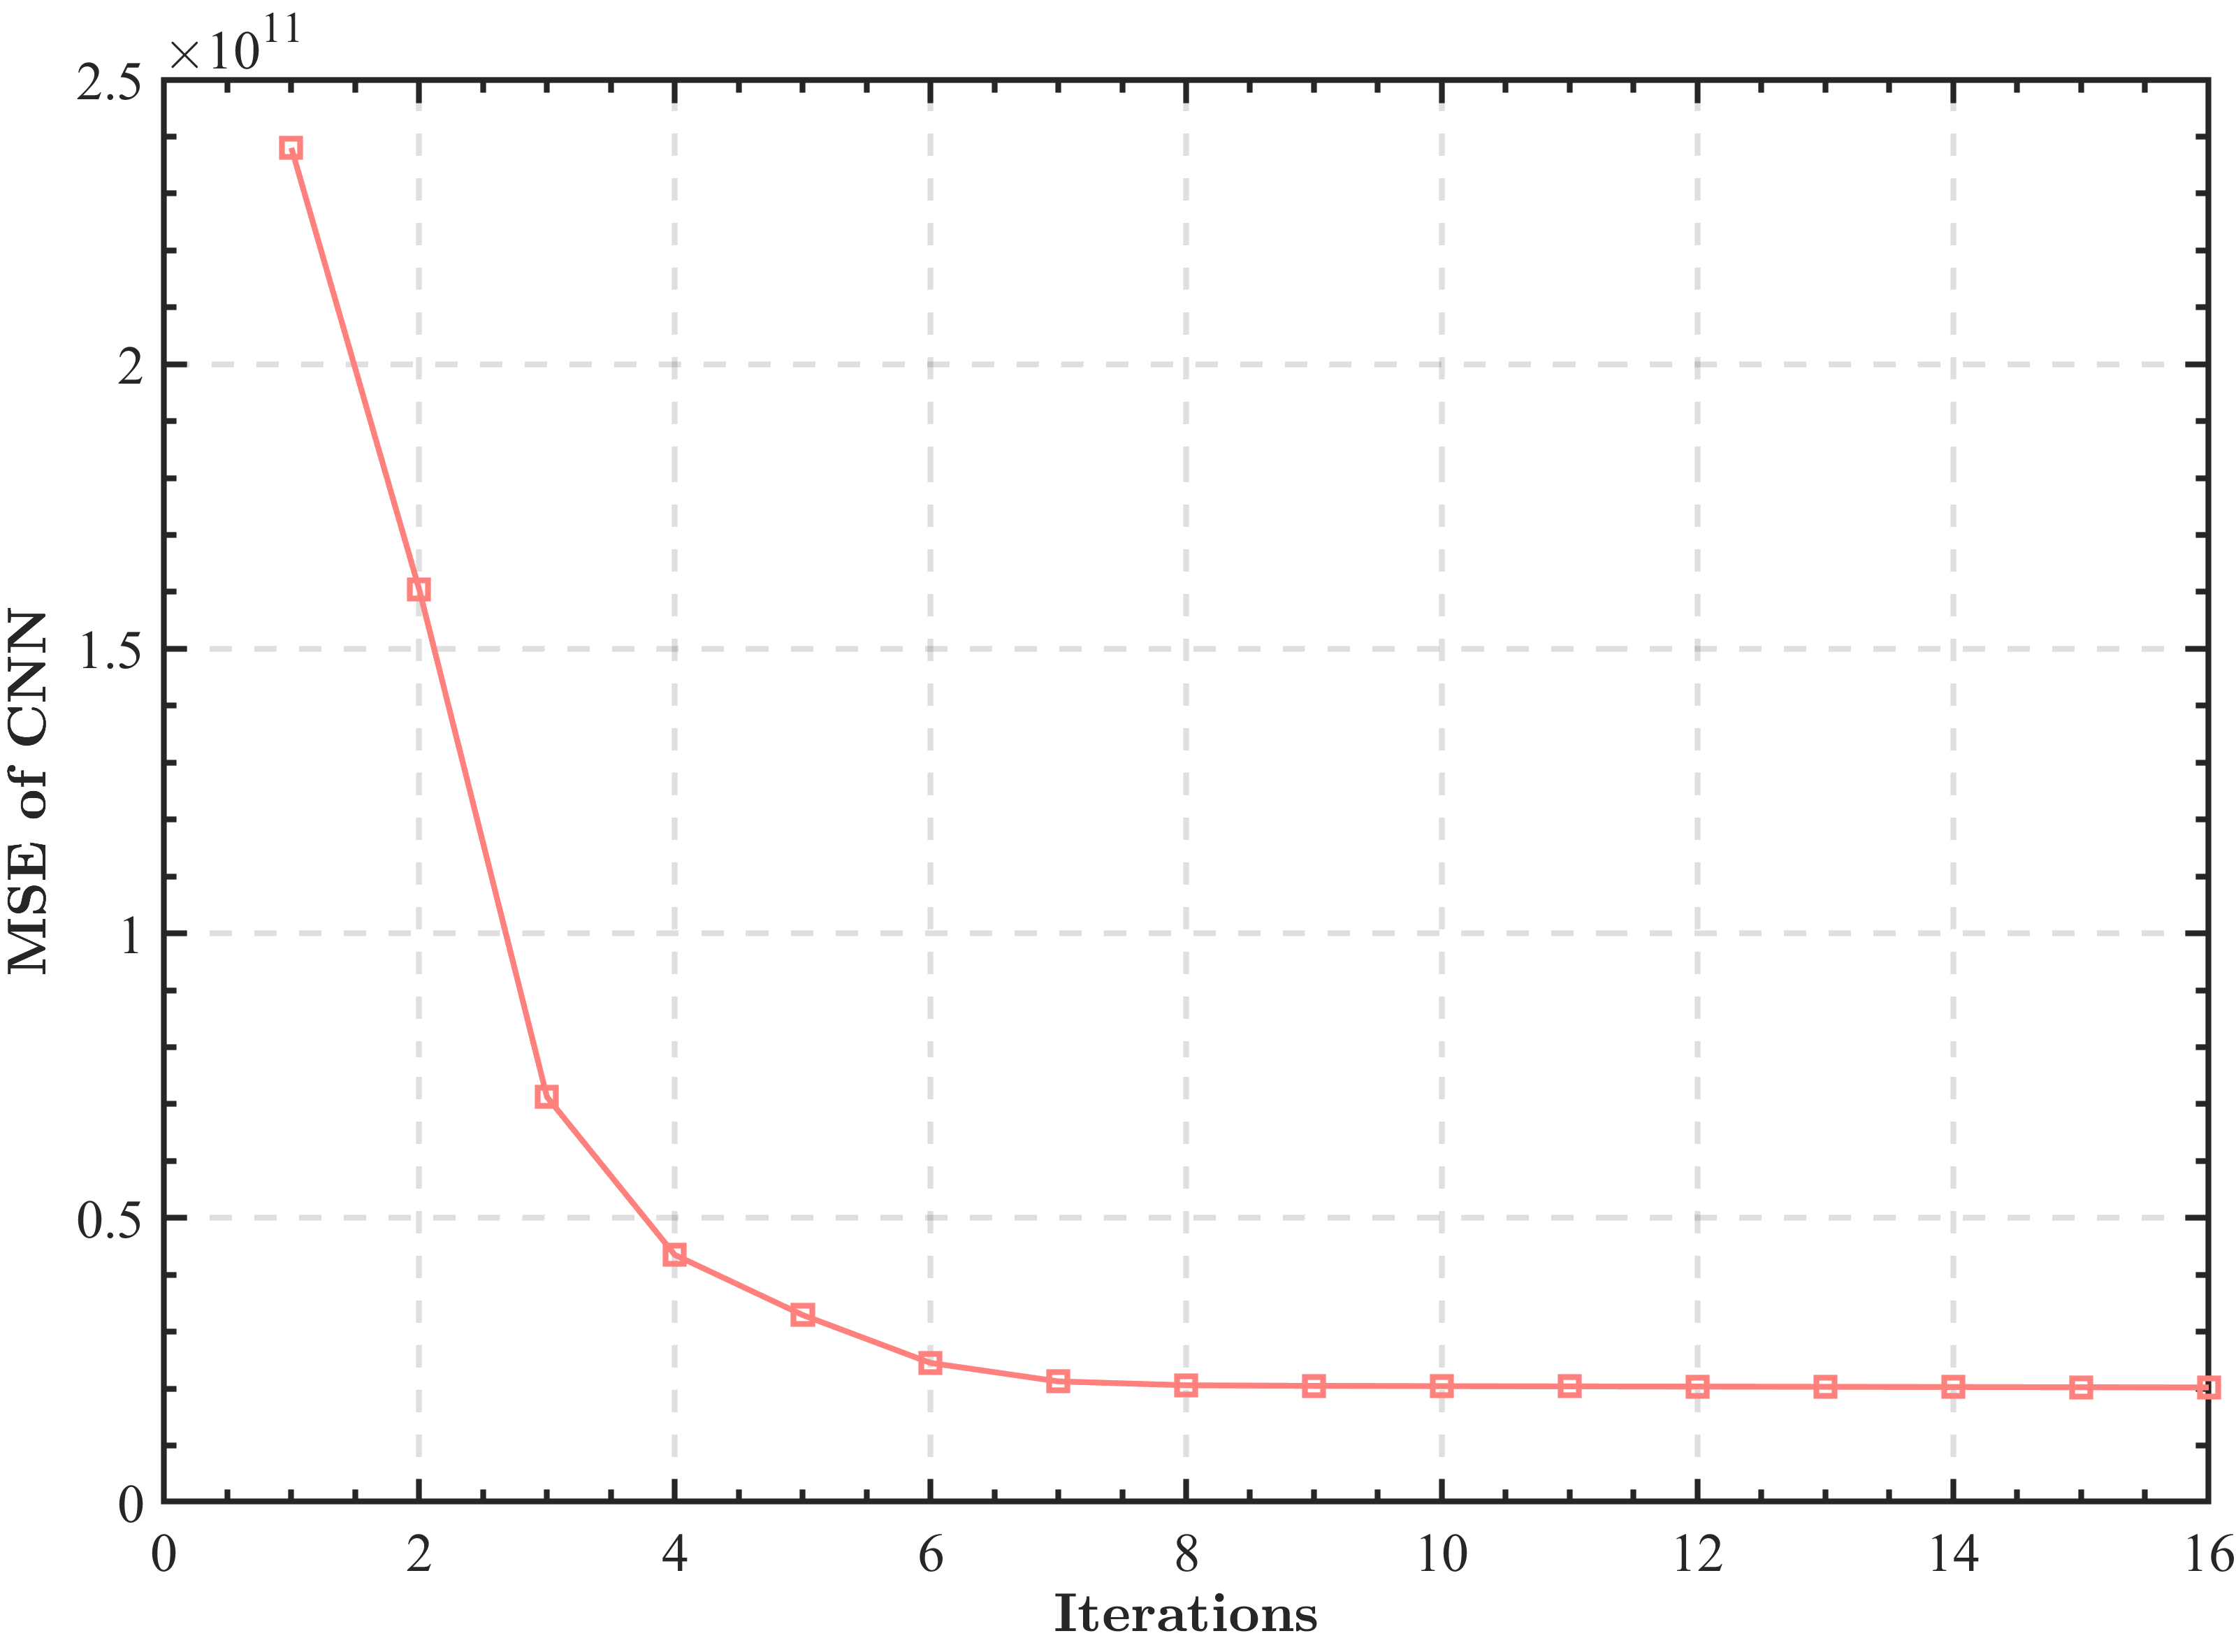
\includegraphics[width=0.30\textwidth]{test_11.png}} 
    \caption{MSE of RF, BP, and CNN Predicted Results} % 图片标题 
\end{figure}
\vspace{-0.5cm}
As can be seen from the figure above, although RF, BP and CNN models have certain predictive functions, their predictive values are not accurate enough and sometimes have large deviations, showing instability. So let's try to mix the models to get a better forecast.

\subsection{Algorithm fusion and fusion model proposed}
In order to further reduce the prediction error, we further adopted the weighted average model fusion method, whose calculation formula is as follows:
\begin{align}
    \overline{\widehat{y}}=\frac{a_1\widehat{y_1}+a_2\widehat{y_2}+a_3\widehat{y_3}}{a_1+a_2+a_3}
\end{align}

Where $a_1$, $a_2$ and $a_3$ are the weights of RF, BP and CNN respectively.
Since there is no code to directly mix and improve the prediction model in MATLAB, pseudo-code is used here to represent the model mixing process.

\begin{algorithm}[H]
    \caption{RF, BP and CNN Model Fusion Pseudo-code}
    \SetAlgoLined
    \KwIn{Predicted value (RF, BP \& CNN) \& Actual value}
    \KwOut{$a_i, i=1,2,3$}
    \emph{\textbf{Definition}: $J=Inf$  \& Create $a_{right}$ matrix to record the values of $a_1$, $a_2$ and $a_3$}\;
    \For{$a_3 = 0 to 1(step = 0.01)$}{
        Define the objective function:
        $f\left( a_1 \right) =\min \left\{ \sum{\left( y-\left( a_1x_1+\left( 1-a_3-a_2 \right) x_2+a_3x_3 \right) \right)}^2 \right\} $\;
        Using function fmincon, solve the optimization problem\;
        When the solution is complete, return the resulting $a_1$ and $f(a_1)$\;
        \If{$f(a_1) < J$}{
            $J<--f(a_1)$\;
            Update $a_{right}$ matrix\;
        } 
    }
  \end{algorithm}

  After integrating the models, we used the mixed model to re-forecast the price and compared it with the actual price as shown in the figure below.
\begin{figure}[H]  %h此处,t页顶,b页底,p独立一页,浮动体出现的位置
    \centering  %图表居中
    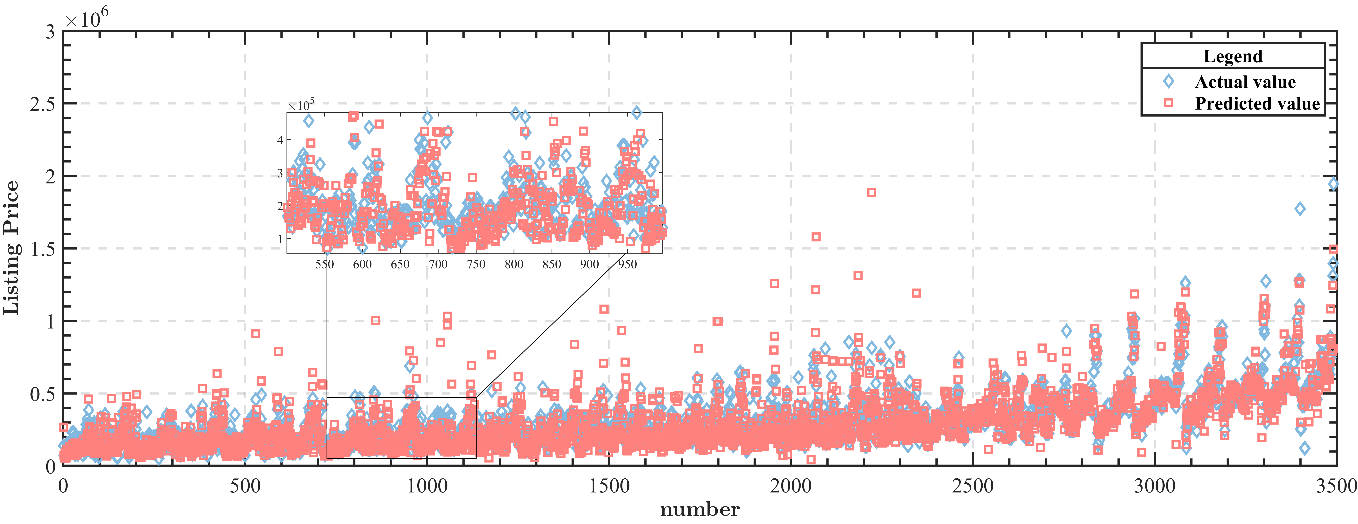
\includegraphics[width=.85\textwidth]{test_12.png} %图片的名称或者路径之中有空格会出问题 
    \caption{Comparison of Prediction Results of Fusion Models} % 图片标题 
    \vspace{-0.5cm}
\end{figure}
%\vspace{-0.5cm}
By comparing the fusion model with the original model, we calculated R2, MSE and Fusion weight, and found that the prediction effect of the fusion model was better than the other three.

\begin{table}[htbp]
    \begin{center}
    \caption{Comparison between the Original Model and the Fusion Model}
    \resizebox{\textwidth}{!} %控制表格整体与文字同宽
    {\begin{tabular}{c c c c}
    \toprule[2pt]
    \multicolumn{1}{m{4cm}}{\centering \textbf{}} %此处表格过小,如果不设置行宽会导致文字变大
    &\multicolumn{1}{m{4cm}}{\centering \textbf{R$^2$}}
    &\multicolumn{1}{m{4cm}}{\centering \textbf{MSE}}
    &\multicolumn{1}{m{4cm}}{\centering \textbf{Fusion Weight}}\\
    %1&R$^2$&MSE&Fusion Weight\\ %可以看情况不使用\multicolumn语法
    \midrule
    RF           & 0.8035 & 1.7178 & 0.284 \\
    BP           & 0.8362 & 1.3248 & 0.562 \\
    CNN          & 0.7824 & 2.0356 & 0.164 \\
    Fusion Model & 0.8818 & 0.8997 &   -   \\
    \bottomrule[2pt]
    \end{tabular}}
    \end{center}
\end{table}
\vspace{-0.5cm}
\subsection{Discussion on the Accuracy of Price Prediction}
In order to estimate the estimation accuracy of our model against price, we first remove the data of the upper and lower quartiles corresponding to the estimation error, and draw a direct statistical graph of the price accuracy according to the remaining data.

\begin{figure}[H]  %h此处,t页顶,b页底,p独立一页,浮动体出现的位置
    \centering  %图表居中
    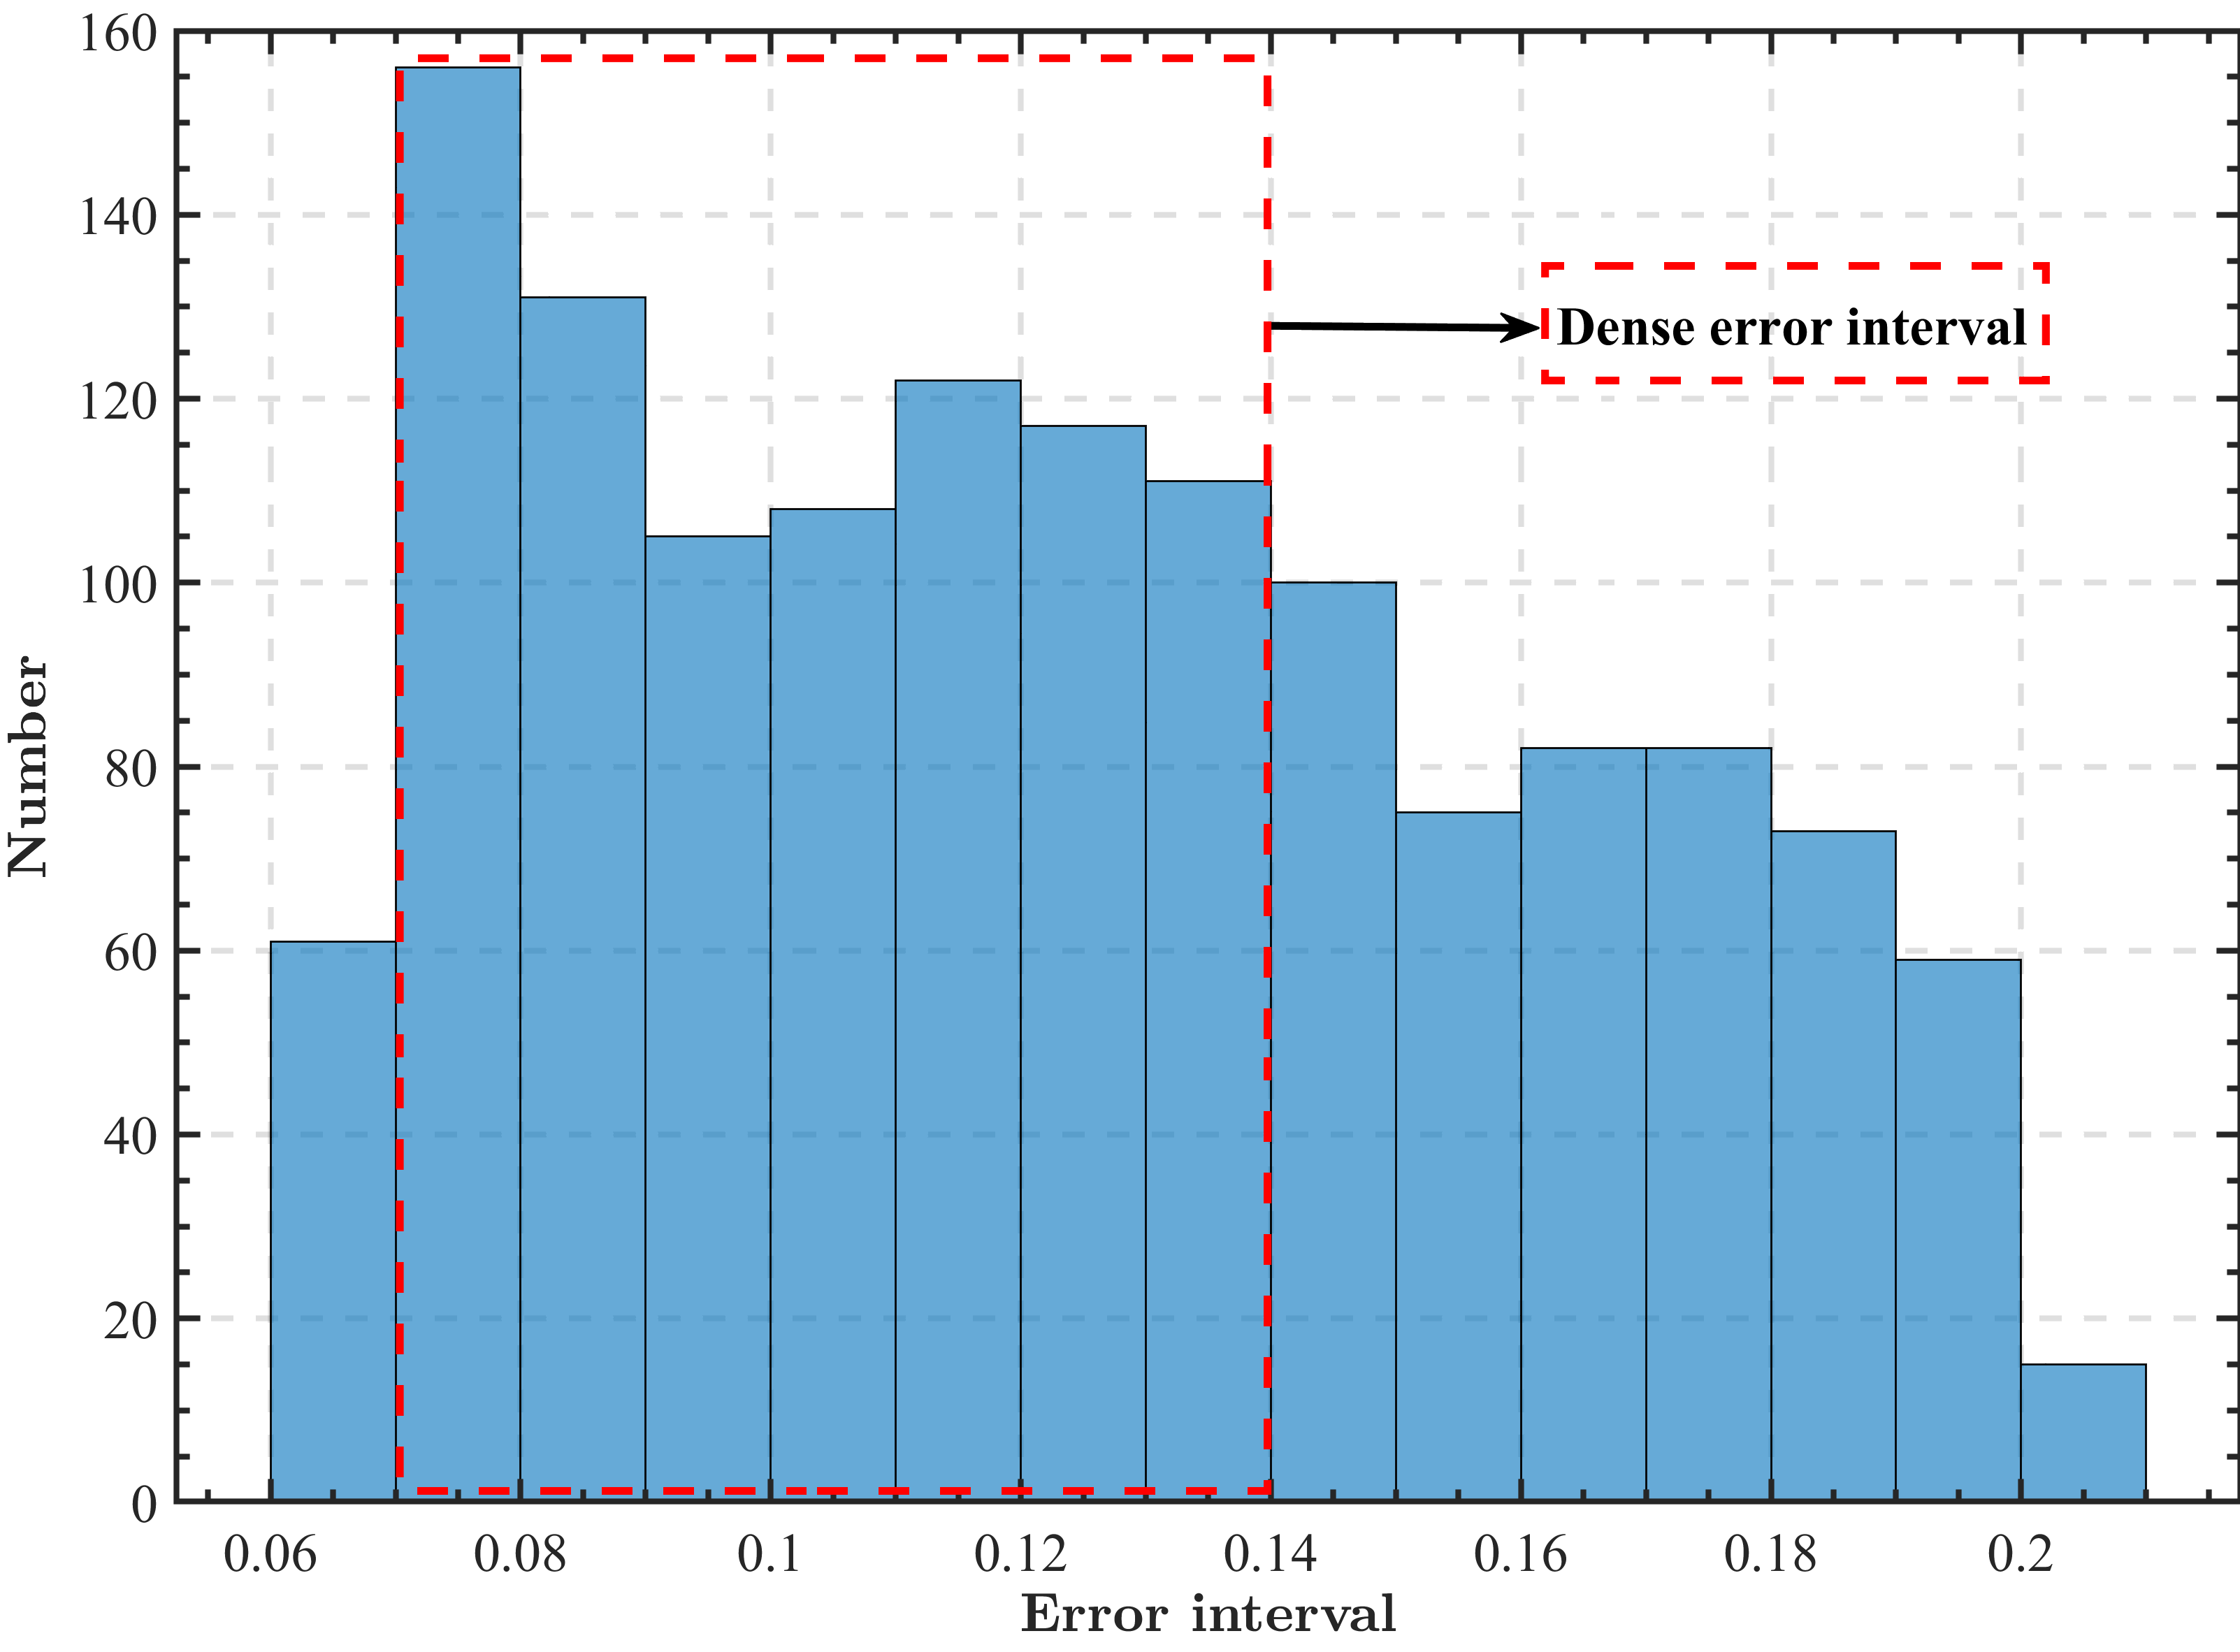
\includegraphics[width=.65\textwidth]{test_13.png} %图片的名称或者路径之中有空格会出问题 
    \caption{Prediction Error of Fusion Model} % 图片标题 
    \vspace{-0.5cm}
\end{figure}

As can be seen from the above figure, the estimated error of our model is concentrated around 7\%-14\%, which has a high accuracy. The average error is 0.1141.


%————————————————————————————————————————————————————————————————————————%
\section{Multiple Regression Analysis Models for Different Regions}
\subsection{Trial Regression of Multiple Regression with Conditional Tests}
Multiple regression is a statistical analysis method that establishes a linear or nonlinear mathematical model of the amount of relationship between multiple variables and uses sam-ple data for analysis.

In order to measure the impact of the area where the sailboat is sold on the price, four indicators were selected for each area as a measure of area. GDP per capita and unemploy-ment rate reflect the local economic level and purchasing power. Average local precipitation and average temperature reflect the environmental requirements of sailing.

Since the magnitude of the indicators can have an impact on the regression analysis, we standardized the data by the following formula.
\begin{align}
    X'=\frac{X-\mu}{\sigma}
\end{align}
We first performed a trial regression to determine the feasibility of the regression, and if Prob>F is less than 0.05, it means that it is significant with 95\% probability. Next we test for heteroskedasticity and the presence of multicollinearity: if Prob>chi2 is less than 0.05 then there is a 95\% probability that the heteroskedasticity exists is significant. If VIF>10, there is significant multicollinearity in the regression. The results are displayed in the table below.
\vspace{-0.5cm}
\begin{table}[H]
    \begin{center}
    \caption{Test Regression and Test Results}
    \resizebox{\textwidth}{!}
    {\begin{tabular}{c c c c}
    \toprule[2pt]
     &Test Regression Results&Heteroskedasticity Test&Multicollinearity Test\\ %可以看情况不使用\multicolumn语法
    \midrule
    Value   & 0.0000 & 0.0990 & 1.56 \\
    Results & Pass   & Fail   & Pass \\
    \bottomrule[2pt]
    \end{tabular}}
    \end{center}
\end{table}
\vspace{-0.5cm}
We found that the data set had significant heteroskedasticity, so we used least squares with robust standard errors for the regression.

\subsection{Calculation of regional effect indicators for all-round sailboats}

We calculated the regression equation based on the Stata software and obtained the co-efficients in the following table.	
\vspace{-0.5cm}
\begin{table}[H]
    \begin{center}
    \caption{Regression Results of Each Indicator}
    \resizebox{\textwidth}{!}
    {\begin{tabular}{c c c c c}
    \toprule[2pt]
    \multicolumn{1}{m{5cm}}{\centering \textbf{}} %此处表格过小,如果不设置行宽会导致文字变大
    &\multicolumn{1}{m{3cm}}{\centering \textbf{Coefficient}}
    &\multicolumn{1}{m{3cm}}{\centering \textbf{Std. err}}
    &\multicolumn{1}{m{2.5cm}}{\centering \textbf{t}}
    &\multicolumn{1}{m{2.5cm}}{\centering \textbf{P>|t|}}\\
    \midrule
    Unemployment rate   & -0.0141 & 0.0189 & -0.75 & 0.456 \\
    Average temperature & 0.1072  & 0.0212 & 5.05 & 0.000\\
    GDP per capita   & 0.0175 & 0.0198 & 0.89 & 0.376\\
    Average precipitation & -0.2754   & 0.0193 & -1.42 & 0.155\\
    Constants & 0.0000 & 0.0168 & -0.00 & 1.000\\
    \bottomrule[2pt]
    \end{tabular}}
    \end{center}
\end{table}
\vspace{-0.5cm}

The coefficients in the above table indicate the degree of influence of the independent variable on the dependent variable. The absolute value of the coefficient reflects the degree of influence on the listing price of the sailboat.

GDP per capita and average temperature are positively correlated with sailboat prices, suggesting that when the economy is higher or the temperature is higher, people are more enthusiastic about water sports such as sailing, which leads to higher sales prices at that time. On the other hand, precipitation and unemployment reduce the sales of sailboats, which leads to lower prices.

From this, we can obtain the corresponding regression equation:
\begin{align}
    y=\sum_{i=1}^4{a_ix_i+C}
\end{align}
Where $a_1$ to $a_4$ represents the coefficient of each indicator.

The equation obtained the regression equation by multiple regression through four re-gional indicators that may affect the price of sailboats, which better describes the influence of region on the listing price of sailboats.

For the regional effects of each sailing variant, we used the coefficients of each indica-tor as weights to calculate the sequential change in prices. Based on the change in their price order we can compare the regional effects of each sailing variant.

\begin{figure}[H]  %h此处,t页顶,b页底,p独立一页,浮动体出现的位置
    \centering  %图表居中
    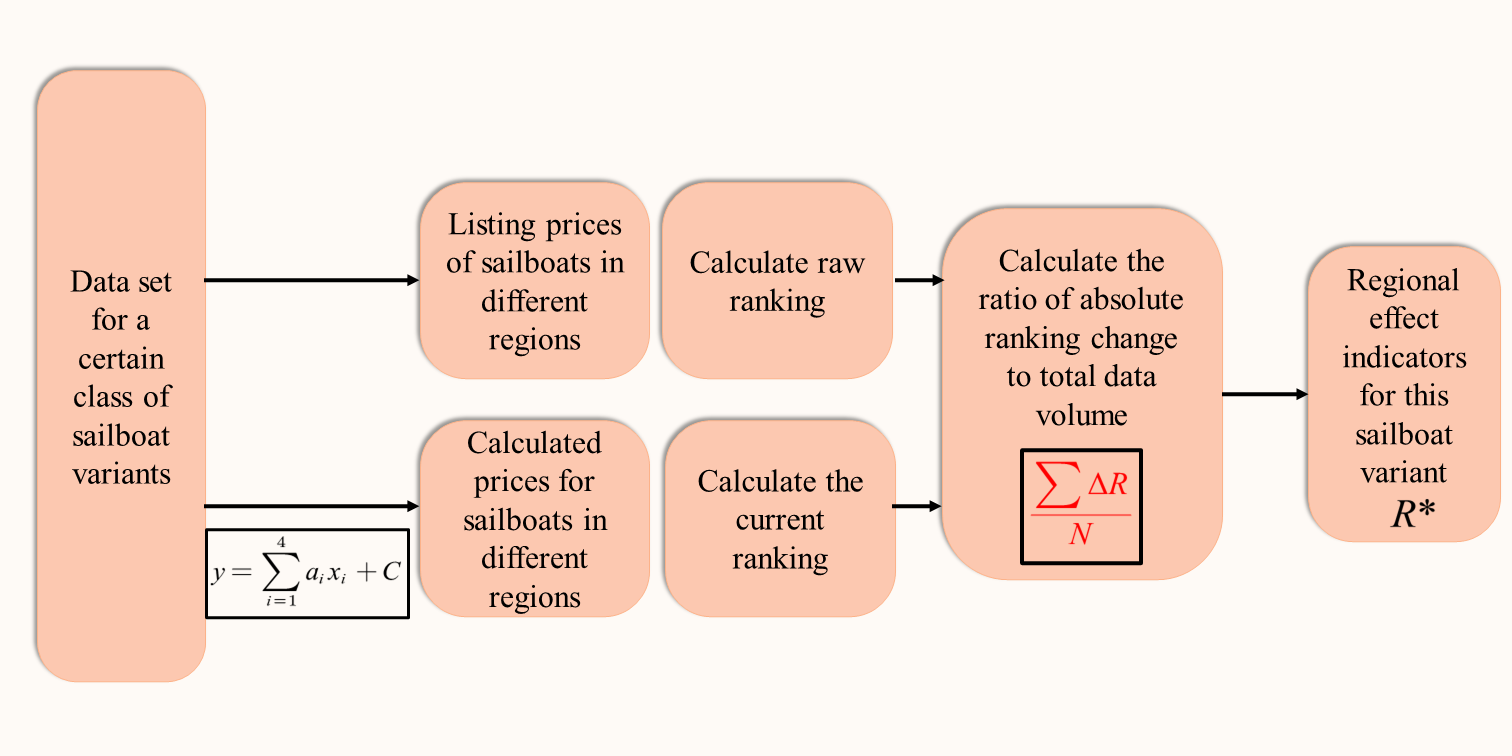
\includegraphics[width=.90\textwidth]{test_14.png} %图片的名称或者路径之中有空格会出问题 
    \caption{ Calculation Method of Regional Effect Indicators} % 图片标题 
    \vspace{-0.5cm}
\end{figure}

This figure shows in detail how the area effect metrics were calculated for the various sailboat variants. By calculating as above, we can obtain the area effect for each sailboat variant.

We noted in our calculations that variants of sailboats sold in only one region do not re-flect a regional effect. Therefore, we rounded off the sailboat types with only one data to obtain the regional effects for each type of sailboat variants as shown in the figure and cal-culated the sailboat models with insignificant regional effects to obtain the table below.
\vspace{-0.5cm}
\begin{figure}[H]
    \centering    
    \subfigure[Division of Different Regional Effects(left)]{				% 图片1([]内为子图标题)						
    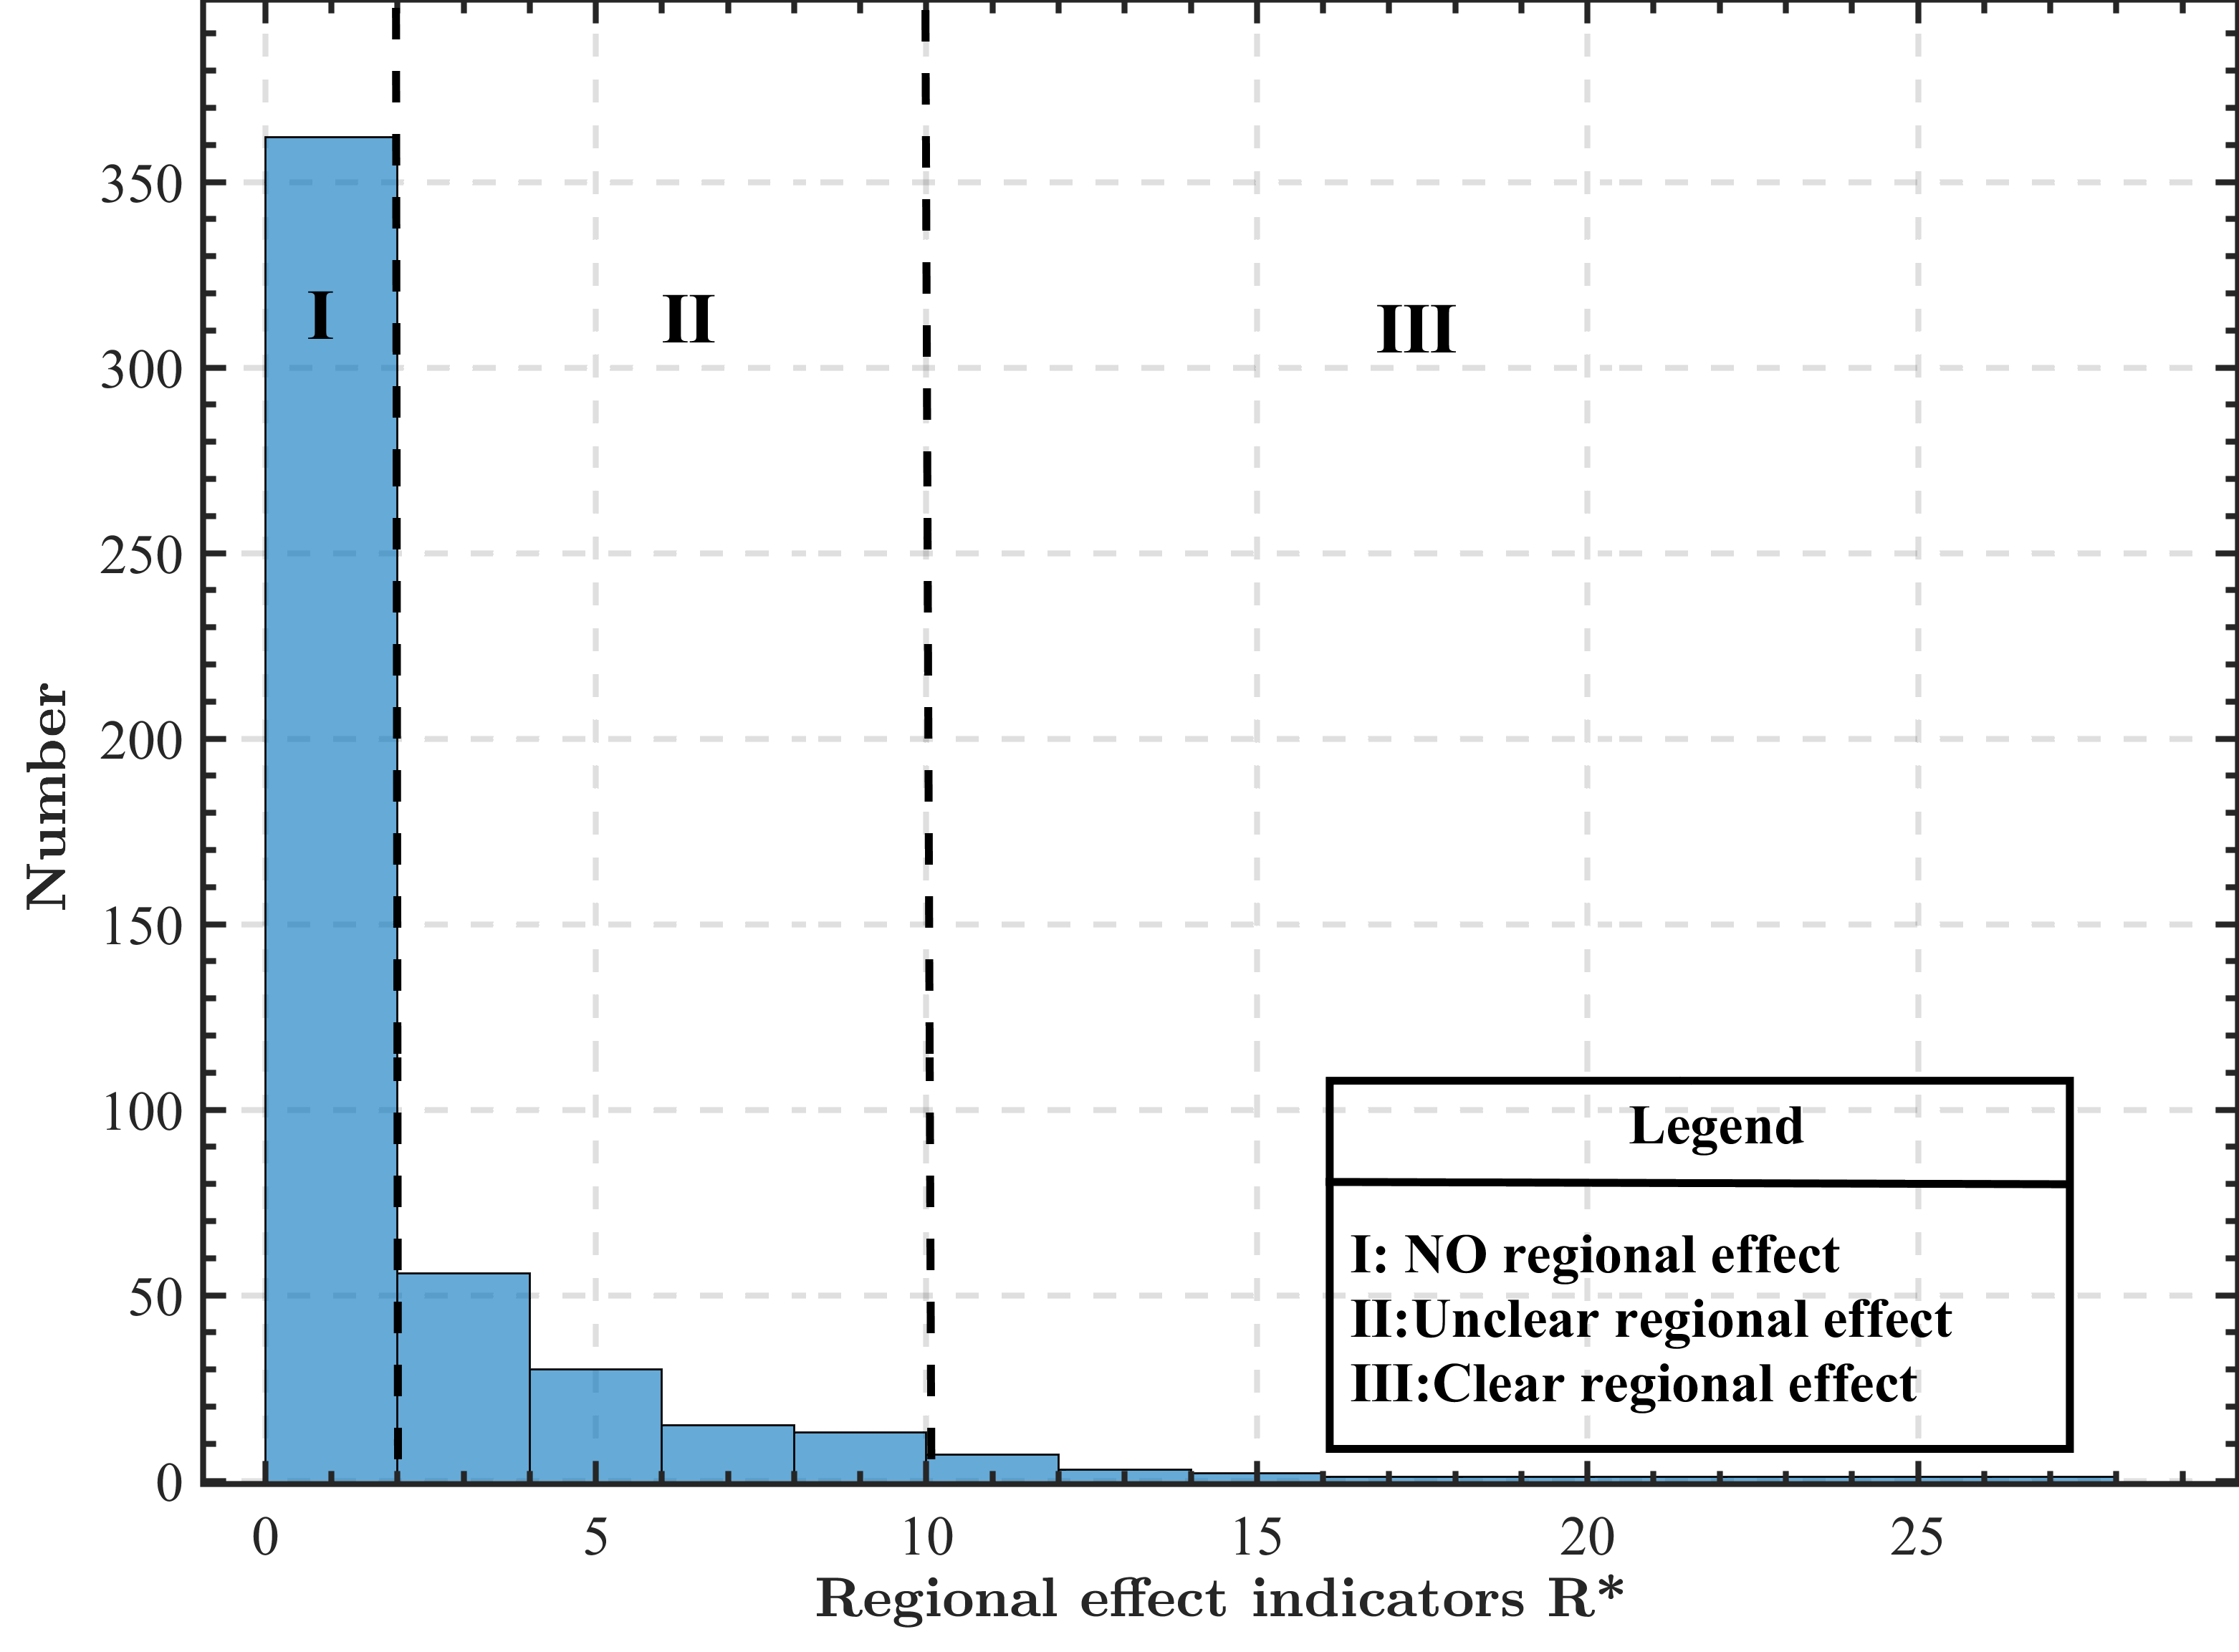
\includegraphics[width=0.45\textwidth]{test_15.png}}			  % 子图1的图片宽度 不能空行
    \subfigure[The Proportion of Different Regional Effects(right)]{				% 图片2
    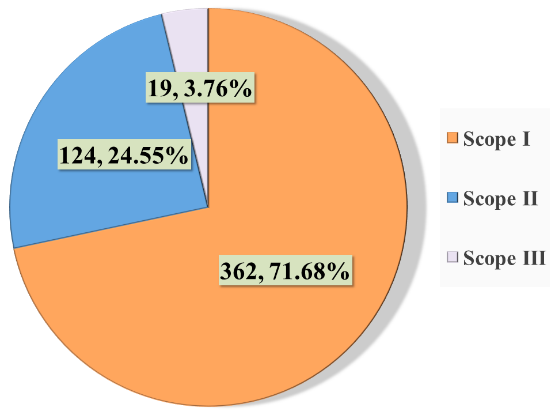
\includegraphics[width=0.45\textwidth]{test_16.png}} 
	\caption{Indicators of Regional Effects of Sailing} % 图片标题 
\end{figure}
\vspace{-0.5cm}
Statistically, there are 19(3.76\%) categories of sailboat variants with obvious regional effects, 124(24.55%) categories of sailboats with insignificant regional effects, and 362(71.68\%) categories of sailboats that do not satisfy the regional effects.

\vspace{-0.5cm}
\begin{table}[H]
    \begin{center}
    \caption{ Types of Sailboats with Large Regional Effects}
    \resizebox{\textwidth}{!}
    {\begin{tabular}{p{4cm} p{4cm} p{4cm} p{4cm}}
    \toprule[2pt]
    \multicolumn{4}{c}{Sailboat variants with insignificant regional effects}\\
    %\multirow{4}*{Sailboat variants with insignificant regional effects}\\
    \midrule
    Hanse 411  & Hanse 461 & Hanse 531 & Hanse 400 \\
    Beneteau Oceanis 40 & Beneteau Oceanis 45  & Beneteau Oceanis 50 & \makecell[c]{Fountaine\\PajotHelia 44} \\
    Dufour 40   & Dufour 385 GL & Dufour 385 & Leopard 40\\
    Leopard 47 & Leopard 43 & Leopard 46 & Leopard 38  \\
    Leopard 39 & Leopard 44 & Leopard 48 & \\
    \bottomrule[2pt]
    \end{tabular}}
    \end{center}
\end{table}
\vspace{-0.5cm}

\subsection{Discussion of Regional Effects of Sailing Variants}
\begin{itemize}
    \setlength{\parsep}{0ex} %段落间距
    \setlength{\topsep}{2ex} %列表到上下文的垂直距离
    \setlength{\itemsep}{1ex} %条目间距
    \item Statistical impactions of regional effects:\\
    As can be seen from the table, the regression coefficients for environmental factors are generally larger, so the impact of the environment on sailboat prices is greater than that of economic factors.
    \item Practical Implications of Regional Effects:\\
    We can see that local unemployment and average precipitation reduce sailboat prices while average GDP and average temperature increase them. Therefore, for sailboat enthusiasts, they can buy a sailboat in the right region to reduce the cost, while for sailboat brokers, they should take these factors into account to increase the total sales and increase the profit.
\end{itemize}

\section{Hong Kong Area Analysis Using BP Neural Network and MLR}
\subsection{Selection of a subset of sailboats}
From the multiple linear regression model in the second question, we can see that the four indicators in different regions have different degrees of influence on the listing price of sailboats, so we assign different weights to each indicator before we do the correlation anal-ysis, specifically: 0.0850, 0.6440, 0.1056, 0.1654.

Since we need to study the regional influence of the selling price of sailboats in Hong Kong, we first select a subset of data from the given data for each of monohull and catama-ran sailboats. And the information of the region is required to be highly correlated with the Hong Kong region. So we calculate the Pearson correlation coefficient for each data in monohull and catamaran separately with the data in Hong Kong region.

The Pearson correlation coefficient describes the degree of linear correlation of two continuous variables and takes values between -1 and 1. -1 means that the two variables are negatively correlated, 0 means that the two variables are uncorrelated, and 1 means that the two variables are positively correlated. It's specific calculation formula is as follows:[7,8]

\begin{align}
    r\left( X,\ Y \right) =\frac{\text{Cov}\left( X,\ Y \right)}{\sqrt{\text{Var}\left[ X \right] \text{Var}\left[ Y \right]}}
\end{align}
In this question, we correlate the data from the Hong Kong region with the cross-sectional data in the dataset. The finalized data set is 175 for monohulls and 348 for catamarans.

\subsection{BP Network Forecast of Used Sailboat Prices in Hong Kong}
Since the price of sailboats in Hong Kong has a large deviation and is not easy to find, we build a network based on the existing data set to predict as the selling price of sailboats in Hong Kong, the specific prediction steps are shown in the following figure:

\begin{figure}[H]  %h此处,t页顶,b页底,p独立一页,浮动体出现的位置
    \centering  %图表居中
    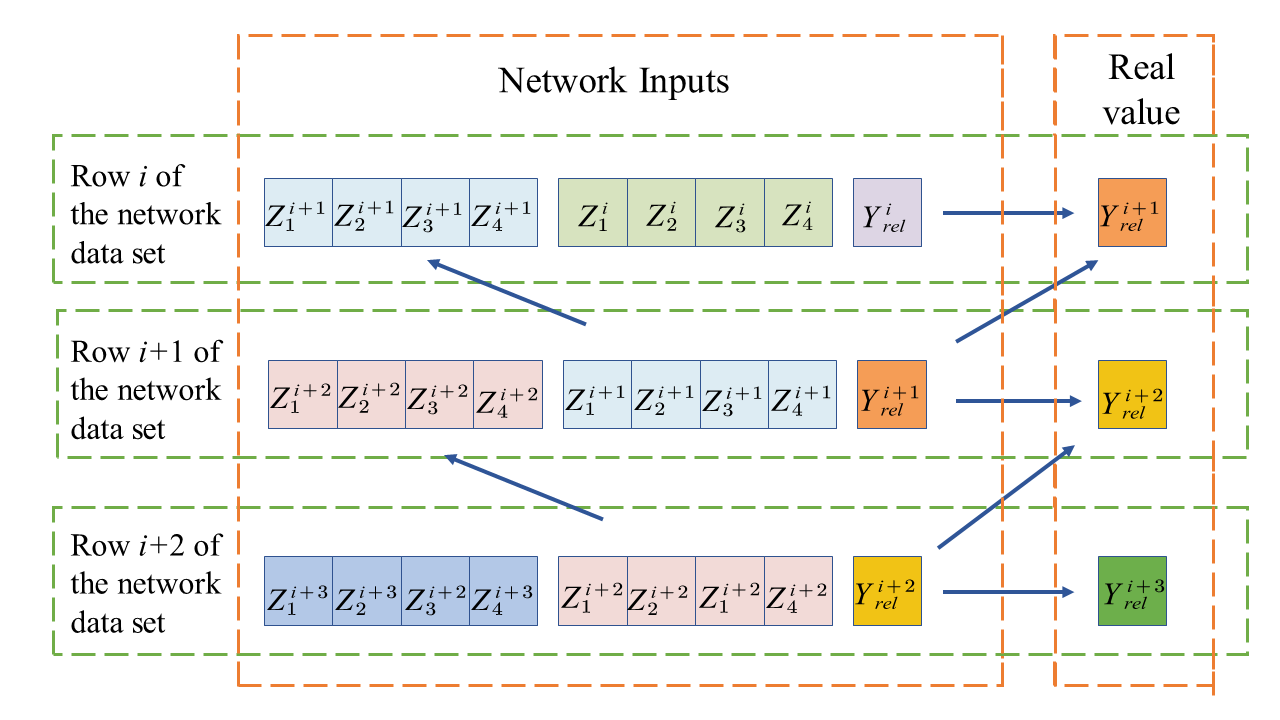
\includegraphics[width=.90\textwidth]{test_17.png} %图片的名称或者路径之中有空格会出问题 
    \caption{Construction of BP Neural Network Dataset} % 图片标题 
\end{figure}
\vspace{-0.5cm}
Where $Z_1^i$ to $Z_4^i$ represents the four regional indicators of a region in row $i$ , and $Y_{rel}^i$B represents the actual sailing price in that region in row i. BP neural network model is built from multiple rows of data.

By constructing the neural network dataset, we bring the dataset into the BP neural network for training and get the following results.

\vspace{-0.5cm}
\begin{figure}[H]
    \centering    
    \subfigure[Monohull Vessels(left)]{				% 图片1([]内为子图标题)						
    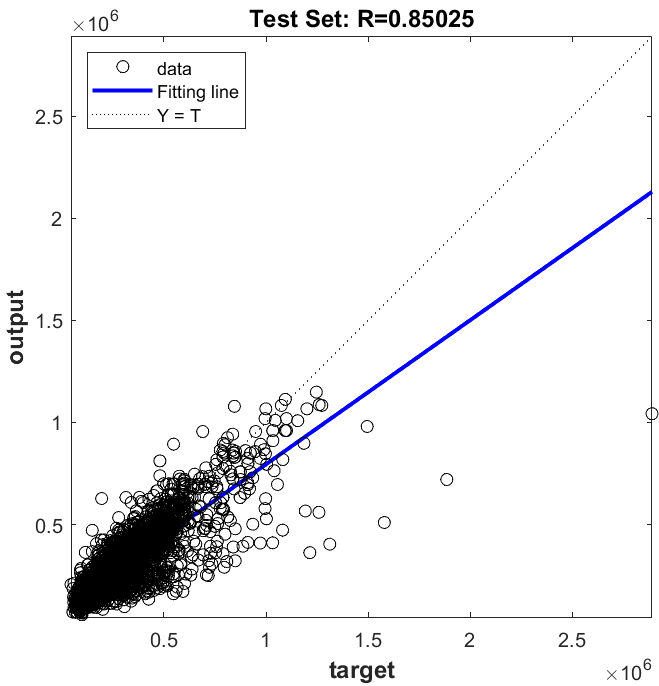
\includegraphics[width=0.41\textwidth]{test_18.png}}			  % 子图1的图片宽度 不能空行
    \subfigure[for Catamarans(right)]{				% 图片2
    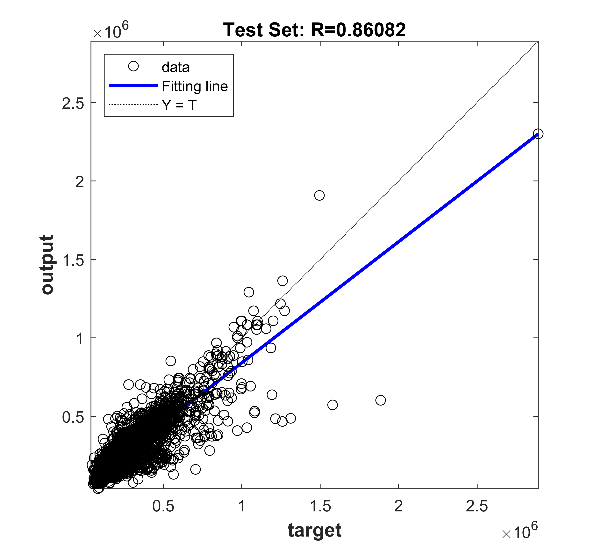
\includegraphics[width=0.49\textwidth]{test_19.png}} 
	\caption{Hong Kong Region Sailing Forecast Results} % 图片标题 
\end{figure}
\vspace{-0.5cm} %这部分两图片不一样大造成排版有问题
It can be seen that the results of the test set for both monohull and catamaran are great-er than 0.85.

We take the regional indicators of Hong Kong, the regional indicators of other regions and the corresponding sailboat prices as inputs for prediction, and get the selling price of this type of sailboat in Hong Kong. If the boat is sold in more than one region then its predicted mean value is taken.

\subsection{Analysis of the regional effects of sailing in Hong Kong}
\subsubsection{Hong Kong Pair Concentration Sailboat Price Impact}

We define the difference between the sailing price in Hong Kong and the sailing price in the original region as $\Delta y$ , and the difference between the regional indicator in Hong Kong and the original regional indicator is noted as $\Delta x_i (i=1,2,3,4)$, respectively. we use the multiple linear regression model of the second question to calculate the regression results for monohull and catamaran sailing boats separately as the following table.

\vspace{-0.5cm}
\begin{table}[H]
    \begin{center}
    \caption{ Types of Sailboats with Large Regional Effects}
    \resizebox{\textwidth}{!}
    {\begin{tabular}{c c c c c c}
    \toprule[2pt]
    \multicolumn{3}{m{8cm}}{\centering \textbf{Monohull}}
    &\multicolumn{3}{m{8cm}}{\centering \textbf{Catamaran}}\\
    %\multicolumn{3}{c}{}
    %&\multicolumn{3}{c}{}\\
    \midrule
      & Coefficient & P>|t| &  & Coefficient & P>|t|\\
    \midrule
    $\Delta x_1$ & -0.059 & 0.461 & $\Delta x_1$ & -0.061 & 0.446\\
    $\Delta x_2$ & 0.169  & 0.008 & $\Delta x_2$ & 0.097  & 0.056 \\
    $\Delta x_3$ & 0.234  & 0.116 & $\Delta x_3$ & 0.125  & 0.152\\
    $\Delta x_4$ & -0.416 & 0.002 & $\Delta x_4$ & -0.189 & 0.000\\
    \bottomrule[2pt]
    \end{tabular}}
    \end{center}
\end{table}
\vspace{-0.5cm}

The results in the table show that for monohull sailboats, the change in average tem-perature and average precipitation has a more significant effect on  , and for catamaran sailboats, the amount of change in average precipitation has a more significant effect on  .

Similarly, we use a similar analysis to the second question to calculate the regional ef-fect of Hong Kong SAR on both subsets of sailboats. We list the sailboat variants for which the Hong Kong SAR effect is more significant in the following table.

\vspace{-0.5cm}
\begin{table}[H]
    \begin{center}
    \caption{Sailboats with a clear regional effect in Hong Kong}
    \resizebox{\textwidth}{!}
    {\begin{tabular}{c c}
    \toprule[2pt]
    \multicolumn{1}{m{8cm}}{\centering \textbf{Monohull}}
    &\multicolumn{1}{m{8cm}}{\centering \textbf{Catamaran}}\\
    \midrule
    Nautitech 40 & Tartan 4300\\
    Catana 47 Ocean Class & Dufour 520 GLO Owner version\\
    Leopard 44 & Elan Impression 45 \\
    Fountaine Pajot SABA50 & \\
    Bali4.6 & \\
    \bottomrule[2pt]
    \end{tabular}}
    \end{center}
\end{table}
\vspace{-0.5cm}


\subsubsection{Regional effects of monohull and catamaran sailing}

To measure whether the regional effects are the same for the subset of monohulls and catamarans in Hong Kong, we cross-tabulate the data for monohulls and catamarans and the model for monohulls and catamarans. The regional effect is the same if the error of bringing the monohull data into the catamaran model is less than 10\%, and vice versa, and the same for the catamaran.

A total of 23 monohulls and 33 catamarans were counted, and the regional effect of Hong Kong on these sailboats is independent of whether they are monohulls or catamarans. We selected these sailing companies for statistics to get the following figure.

\vspace{-0.5cm}
\begin{figure}[H]
    \centering    
    \subfigure[Monohull Company(left)]{				% 图片1([]内为子图标题)						
    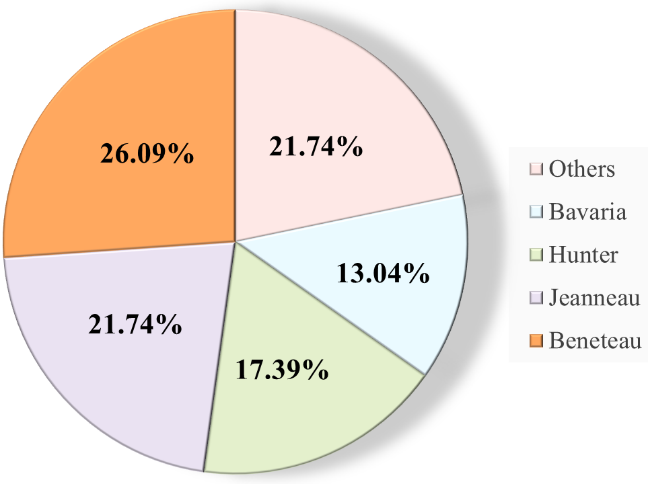
\includegraphics[width=0.43\textwidth]{test_20.png}}			  % 子图1的图片宽度 不能空行
    \subfigure[Catamaran Company(right)]{				% 图片2
    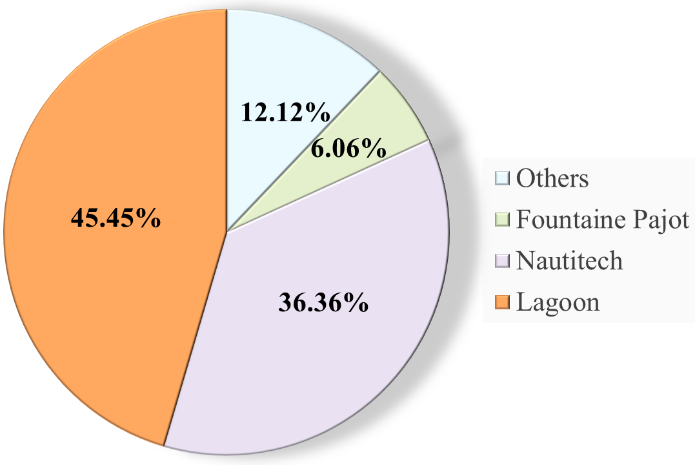
\includegraphics[width=0.47\textwidth]{test_21.png}} 
	\captionsetup{justification=centering} 
    \caption{The Hong Kong region has a consistent impact on \protect\\ whether the company produces monohull vessels} % 图片标题 
\end{figure}
\vspace{-0.5cm} %这部分两图片不一样大造成排版有问题

From the figure we can see that the monohulls similar to Hong Kong area are mainly Bavaria, Hunter, Jeanneau and Beneteau. The catamarans similar to Hong Kong area are Fountaine Pajot, Nautitech and Lagoon.





\section{Conclusions and Interesting Information}
In order to find meaningful conclusions in this data set, we divided the data in terms of manufacturers of sailboats, and conducted statistics and analysis through both sales and prices to draw the following conclusions.
\subsection{Useful and Meaningful Conclusions}
\begin{itemize}
    \setlength{\parsep}{0ex} %段落间距
    \setlength{\topsep}{2ex} %列表到上下文的垂直距离
    \setlength{\itemsep}{1ex} %条目间距
    \item As we can see from the US regional current figure and US sailboat sales data, the US has a long coastline but few ports. It is also affected by the California cold current and the Mexican warm current, which are not conducive to sailing.
    \item We define companies with sales greater than 100 over the last 15 years as large companies and companies with sales less than 10 as small companies. By compar-ing the sailboat sales of large and small companies, we can see that large compa-nies are growing more steadily but small companies are showing a decreasing trend.
    \item For the selling price of sailboats in different regions, we found that some of the same type of boats are selling at a relatively stable price across regions, while others show a large variation across regions. We suspect that the difference be-tween regions may be due to higher transportation costs
\end{itemize}

\begin{figure}[H]
    \centering    
    \subfigure[U.S. Ocean Current Map]{				% 图片1([]内为子图标题)						
    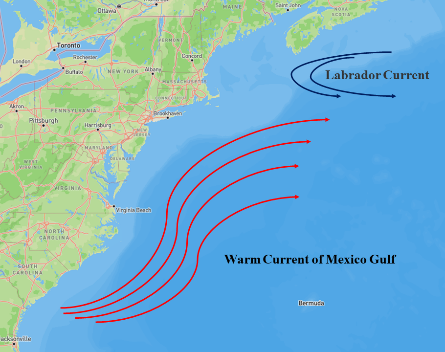
\includegraphics[width=0.30\textwidth]{test_22.png}}			  % 子图1的图片宽度 不能空行
    \subfigure[Large vs. Small Companies]{				% 图片2
    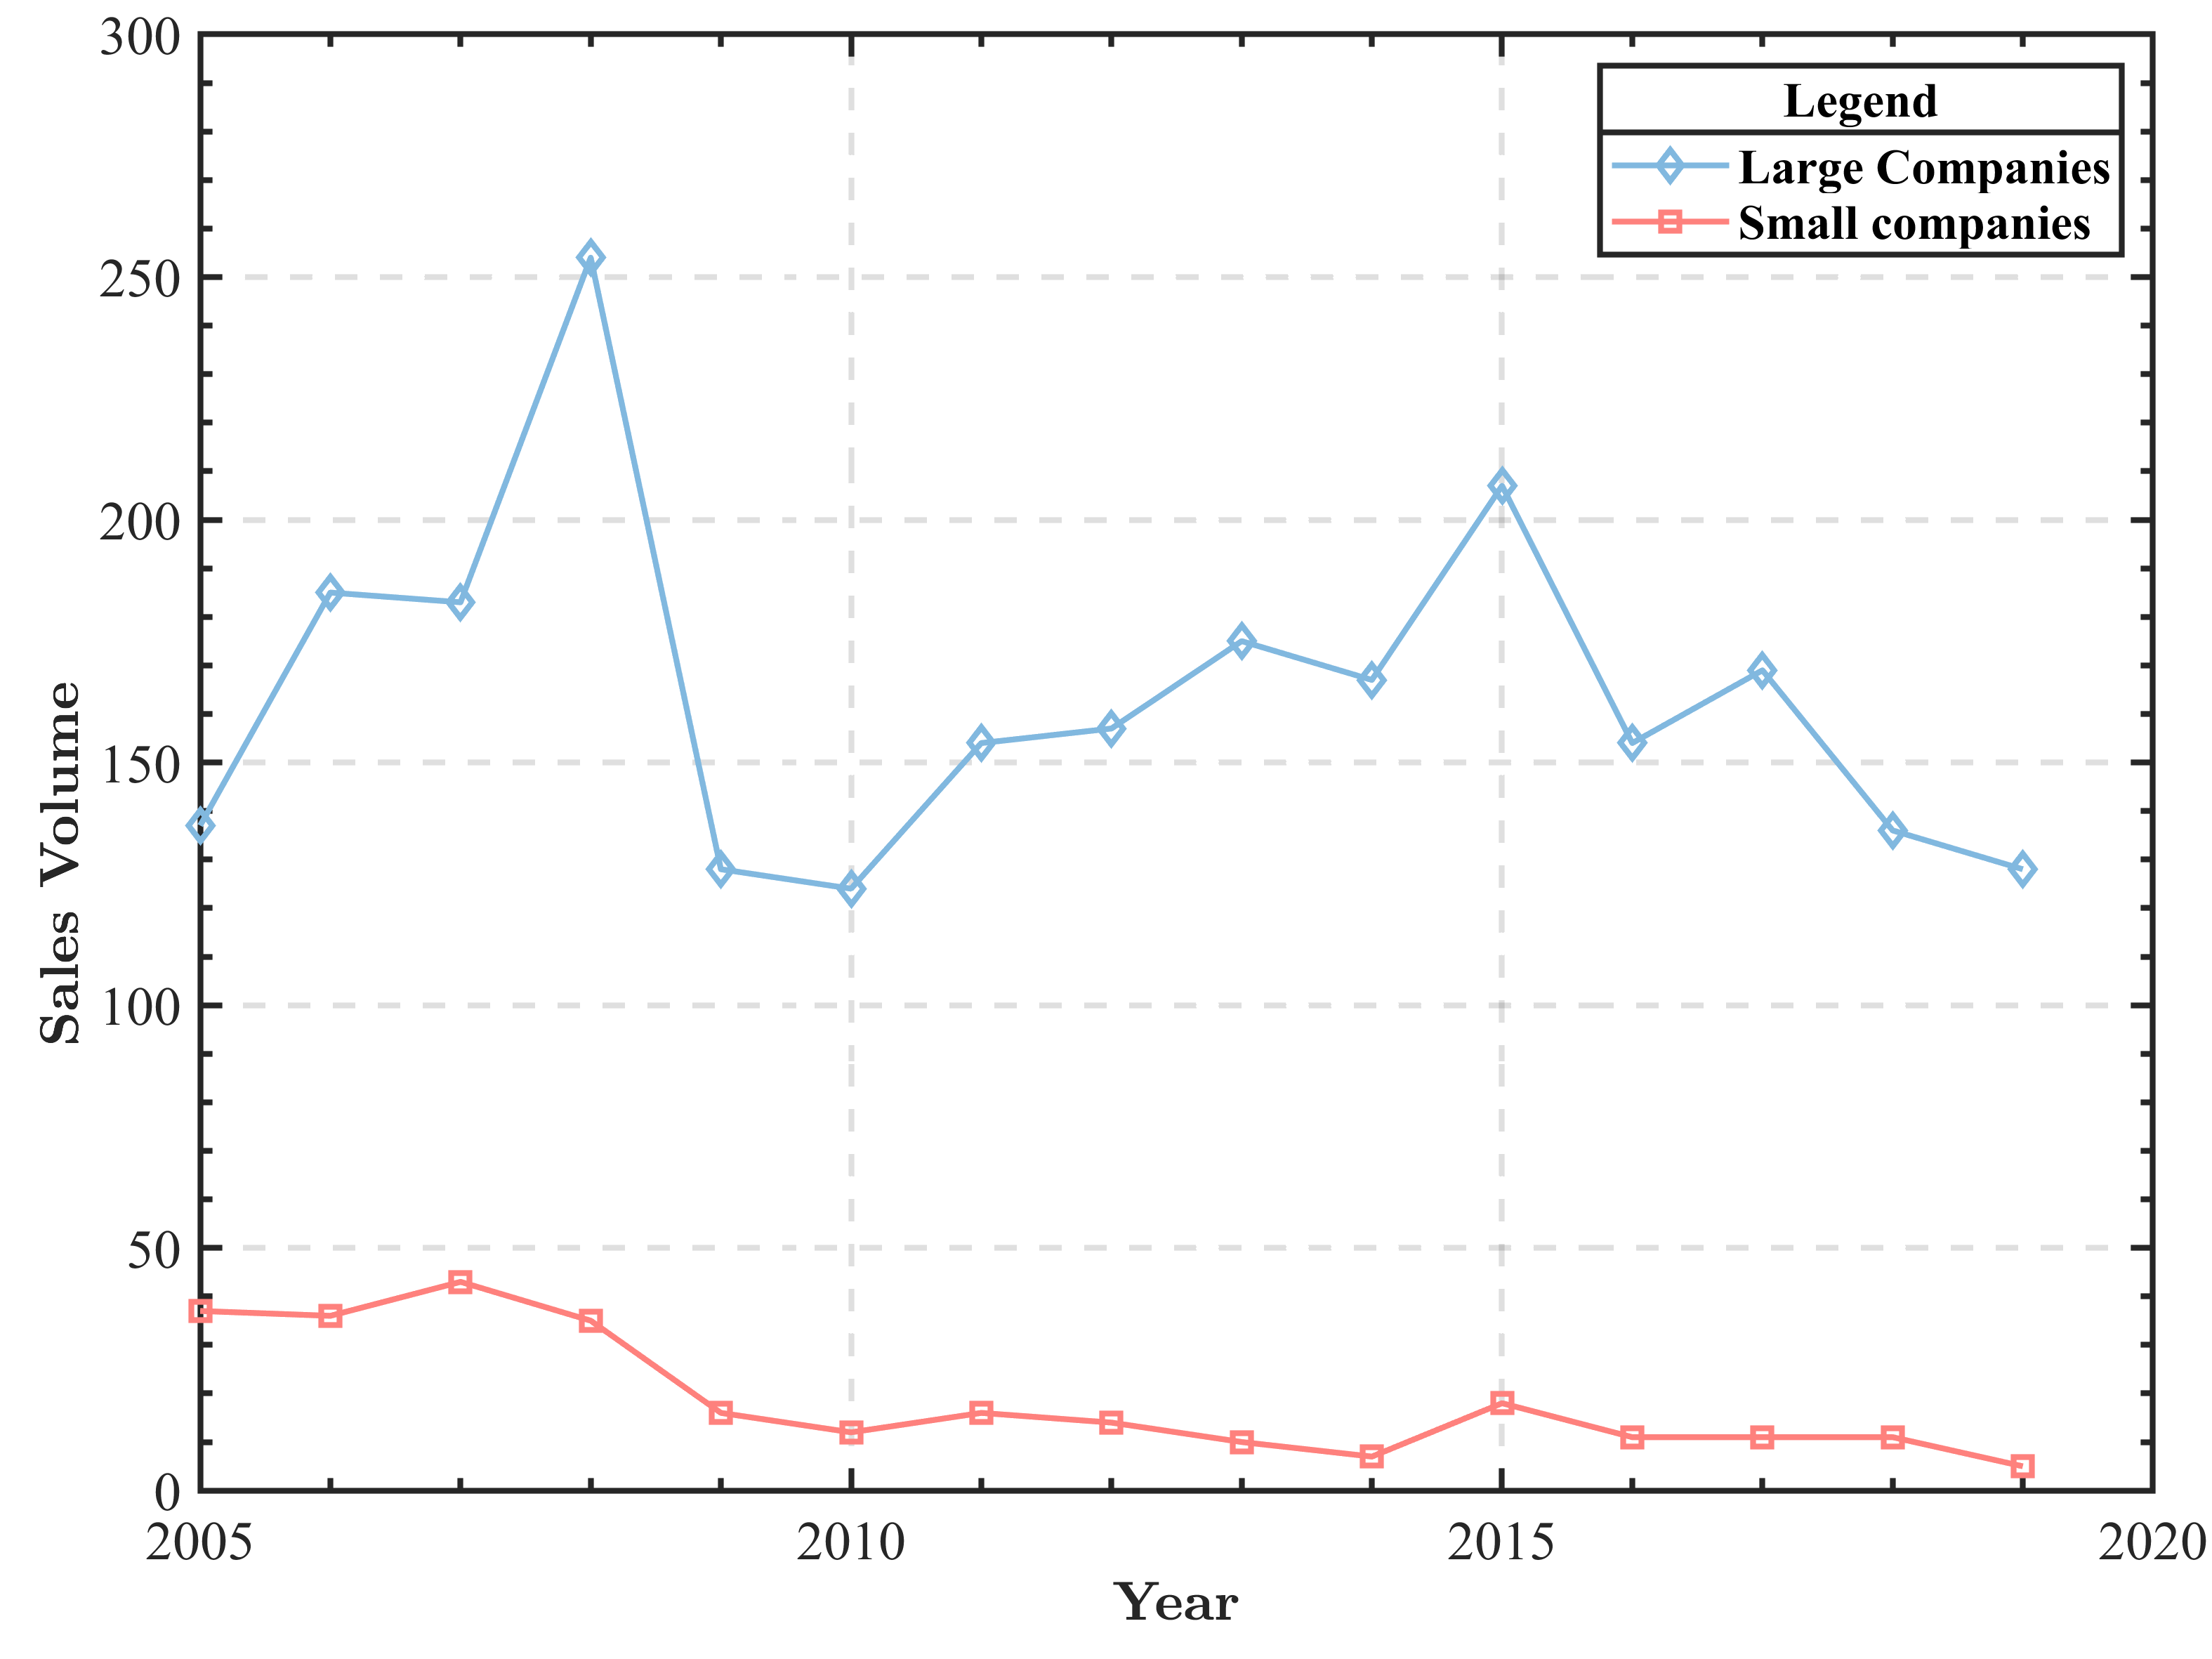
\includegraphics[width=0.315\textwidth]{test_23.png}} 
    \subfigure[Sales Price Stability]{				% 图片2
    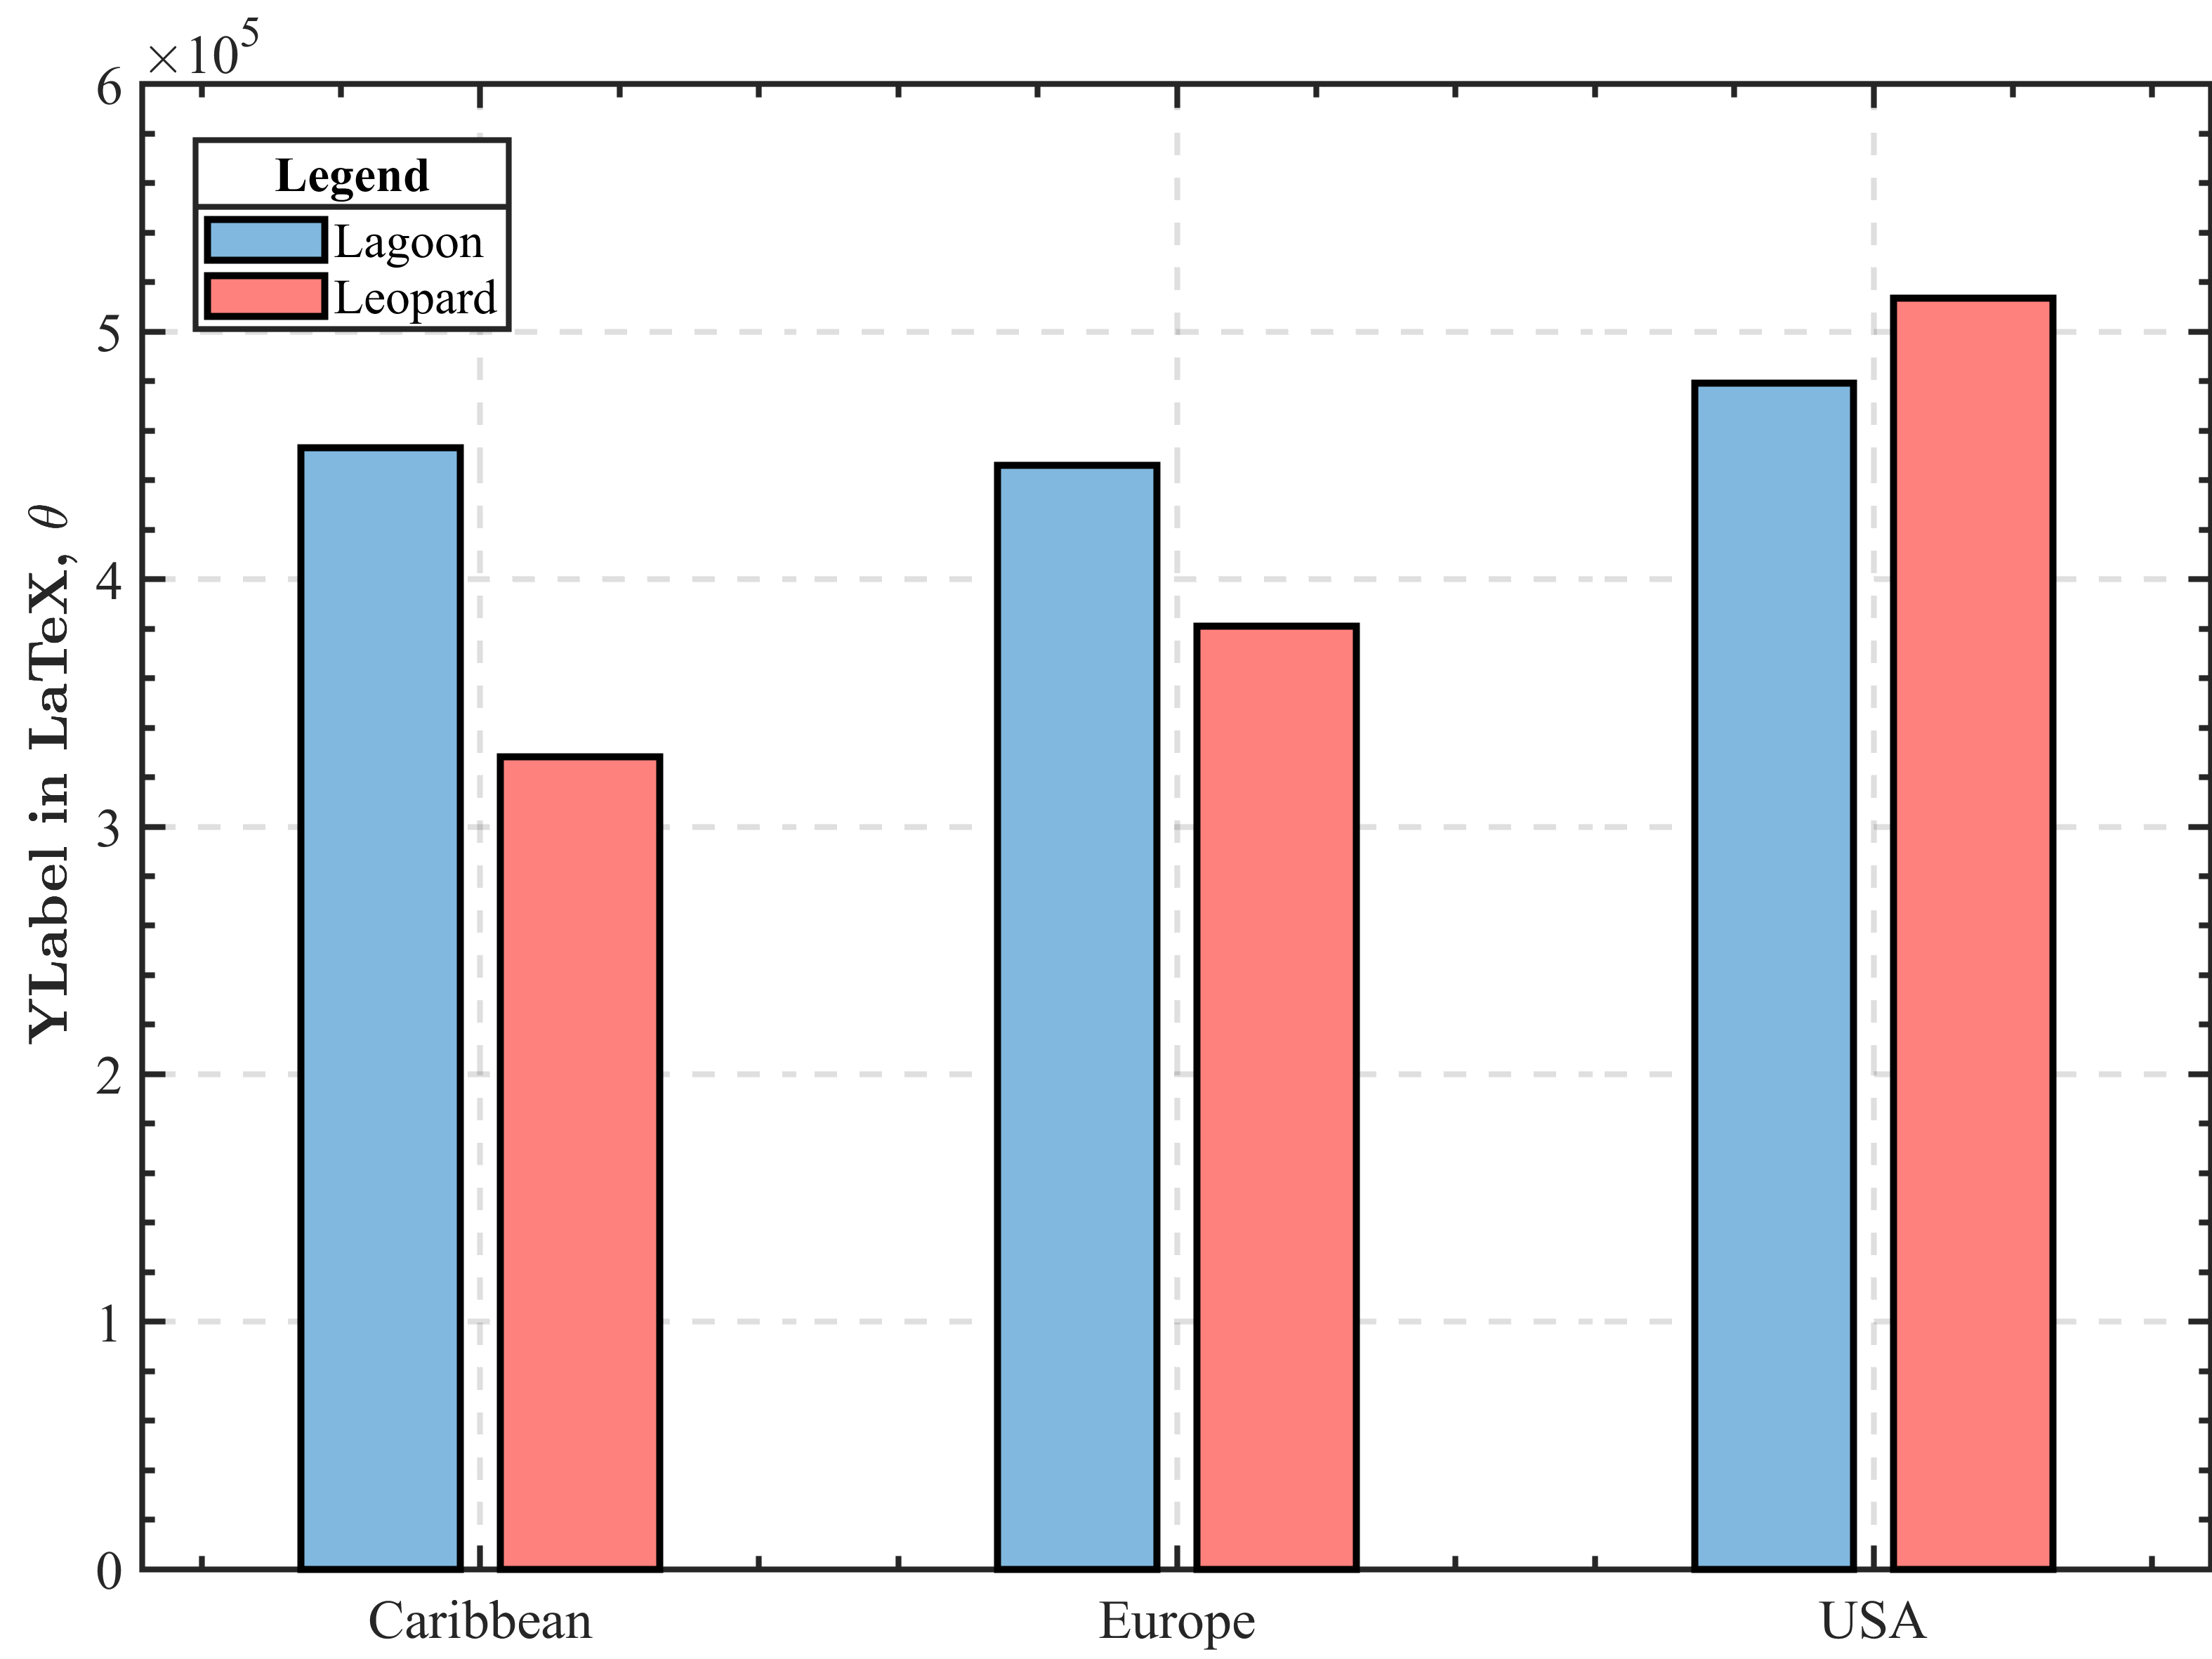
\includegraphics[width=0.315\textwidth]{test_24.png}} 
	\caption{RF, BP, and CNN Predicted Results Compared} % 图片标题 
    \vspace{-0.5cm}
\end{figure}

\subsection{Interesting Conclusions}
\begin{itemize}
    \setlength{\parsep}{0ex} %段落间距
    \setlength{\topsep}{2ex} %列表到上下文的垂直距离
    \setlength{\itemsep}{1ex} %条目间距
    \item We performed a year-by-year statistical comparison of used sailboats of monohull and double hulls. We found that the sales of monohulls are decreasing year by year while the number of catamarans is increasing year by year. This may be related to the increasing level of economic development and quality of recreation in different places.
    \item To explore the market for sailboats, we define sailboats that sell in each year and have an average selling price greater than \$500,000 as high-end market sailboats. Similarly, those with an average selling price of less than \$200,000 are called low end market sailboats.
    \item Our analysis of the annual sales of sailboats shows that some of them (e.g. Solona) alternate between sales and non-sales effects. We speculate that they may run an alternating sales-manufacturing operating model.
\end{itemize}

\begin{figure}[H] %[H]让图片在文章中的位置就是这段代码的位置
	\centering
		\begin{minipage}[t]{0.3\linewidth} %并排排列图片使用\minipage{}环境,而子图排列使用\subfigure{}环境
			\centering
			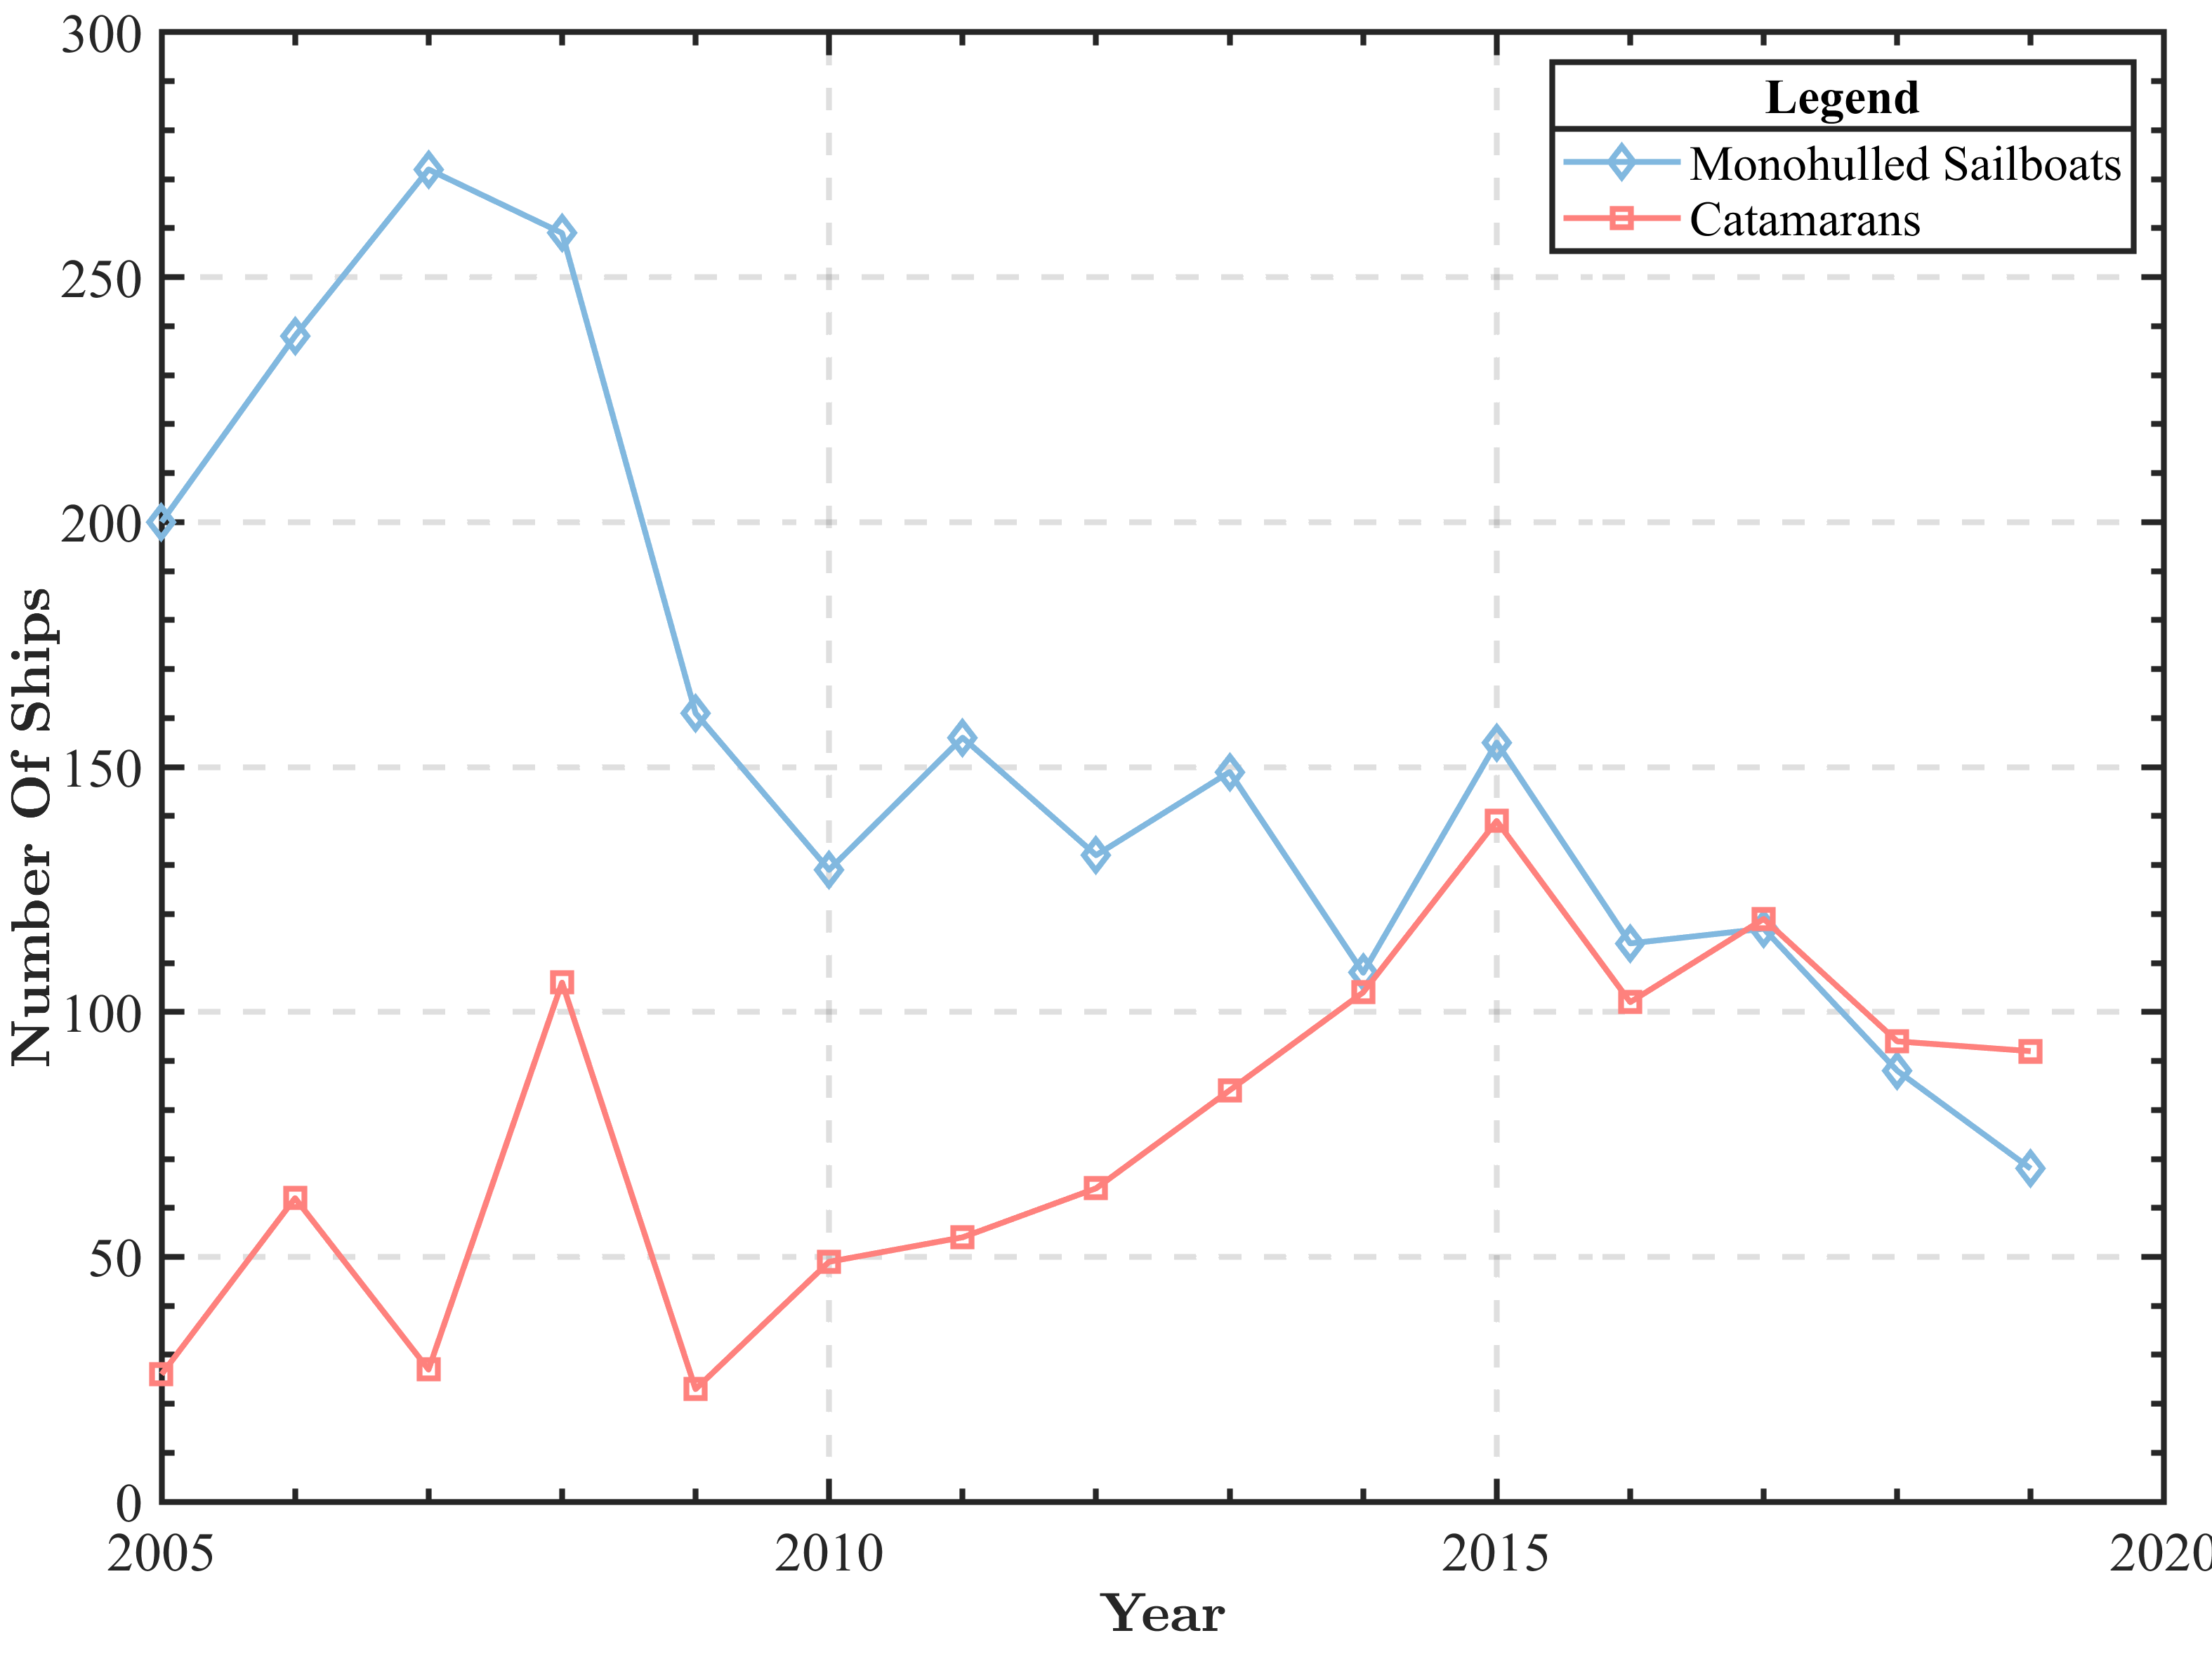
\includegraphics[width=0.9\linewidth]{test_25.png}
            \captionsetup{justification=centering} \caption{Monohull and Catamaran Trends}
		\end{minipage}%
		\begin{minipage}[t]{0.3\linewidth}
			\centering
			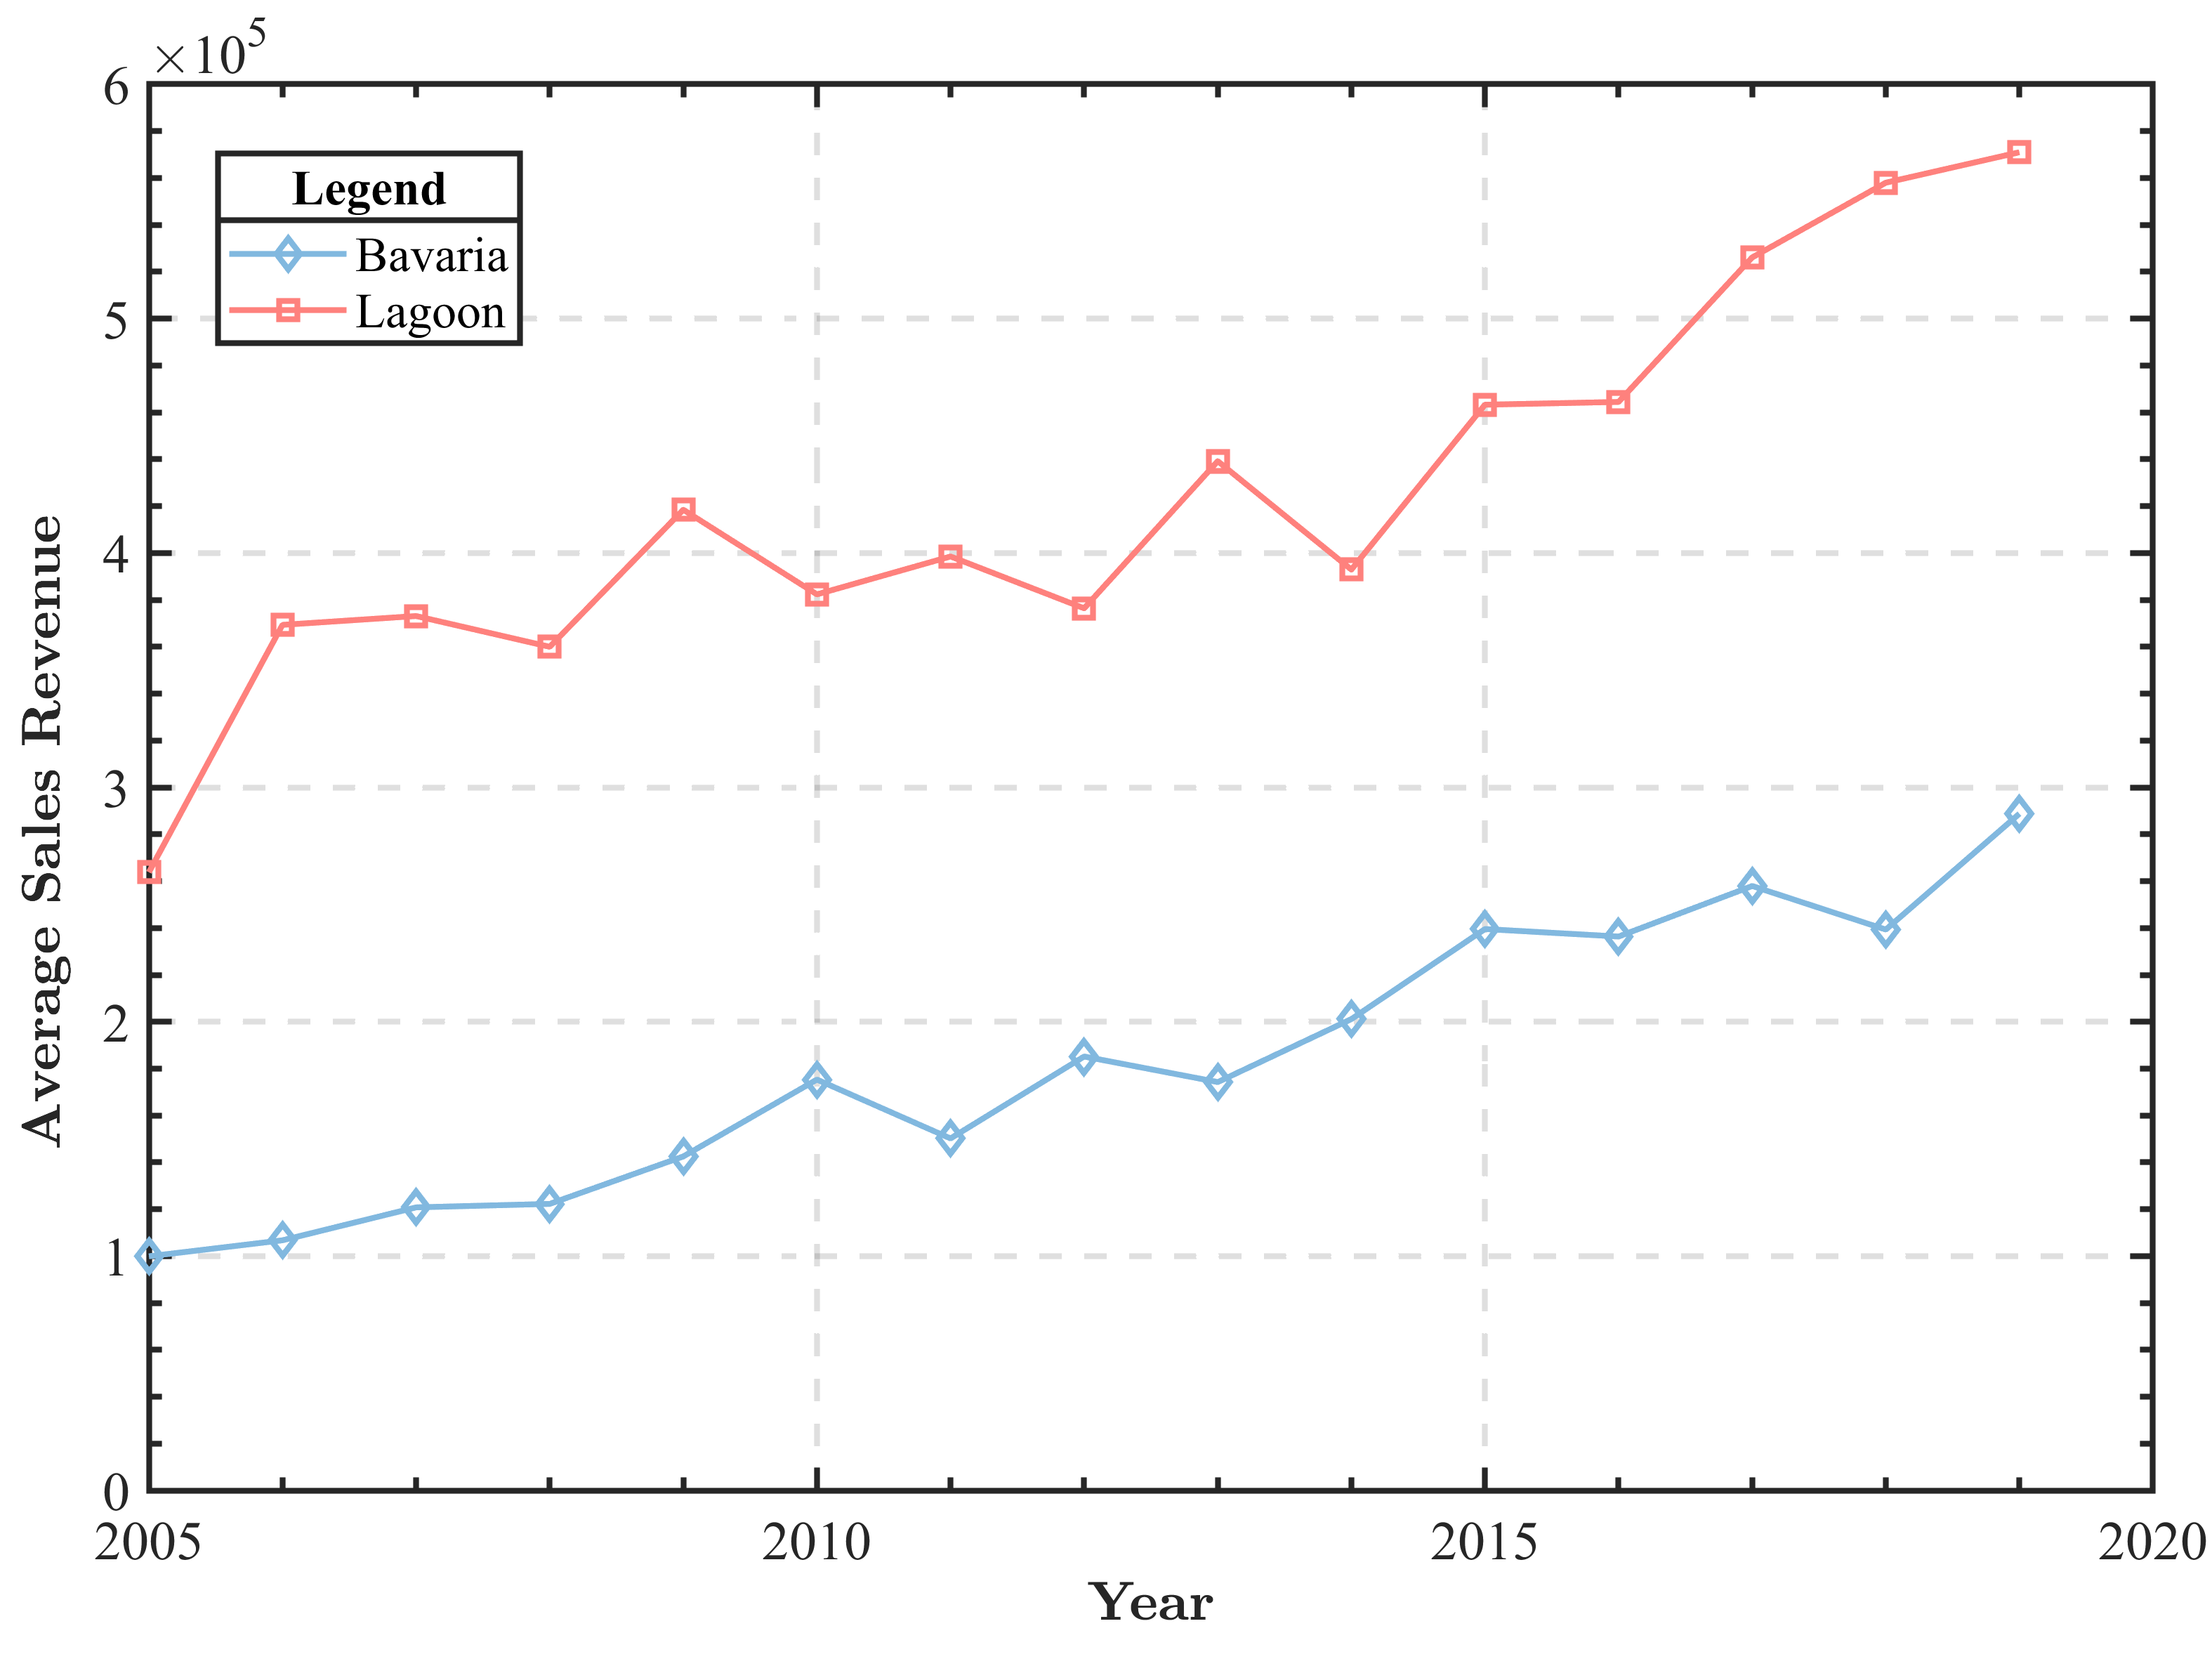
\includegraphics[width = 0.9\linewidth]{test_26.png}
			\captionsetup{justification=centering} \caption{A Comparison of the High and Low End of the Sailing Market}
		\end{minipage}%
        \begin{minipage}[t]{0.3\linewidth}
			\centering
			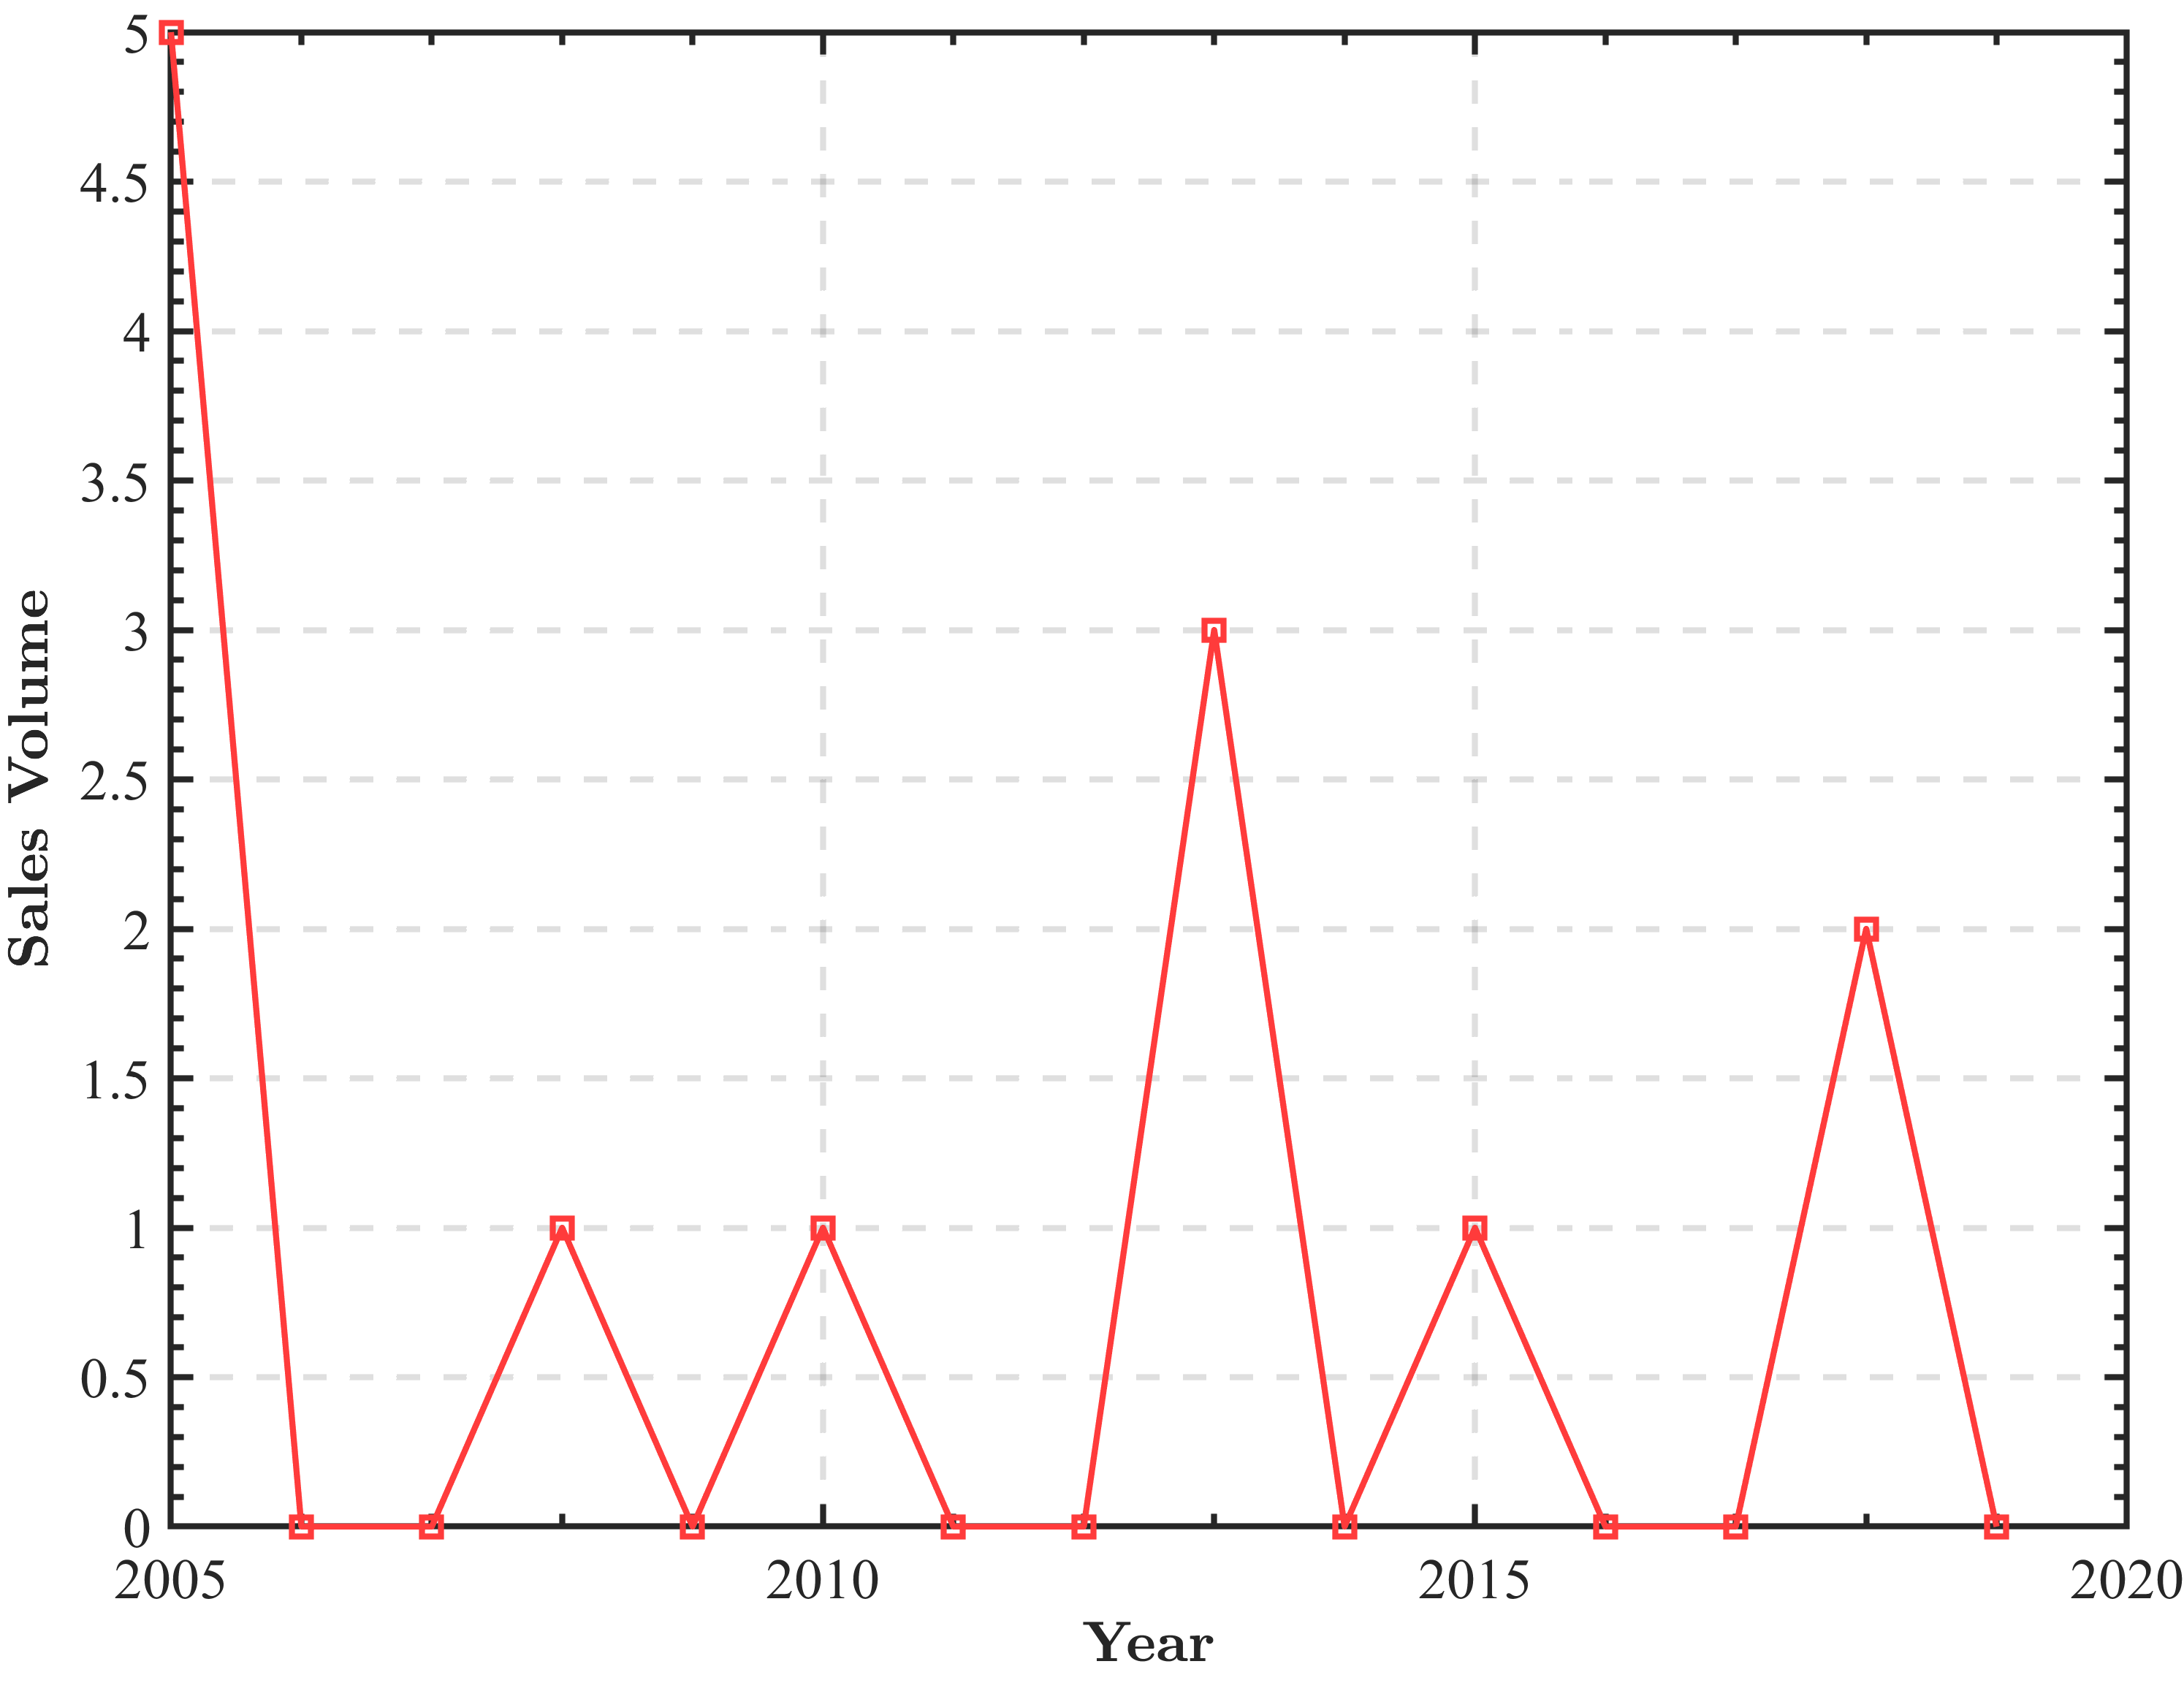
\includegraphics[width = 0.9\linewidth]{test_27.png}
			\captionsetup{justification=centering} \caption{ Solona Sales}
		\end{minipage}%
    \vspace{-0.5cm}
\end{figure}



\section{Sensitivity Analysis}
To verify the robustness of the model, we observe the changes by changing the input val-ues of the neural network.

\begin{itemize}
    \setlength{\parsep}{0ex} %段落间距
    \setlength{\topsep}{2ex} %列表到上下文的垂直距离
    \setlength{\itemsep}{1ex} %条目间距
    \item Sensitivity analysis of the fusion model\\
    We performed a sensitivity analysis of the fusion model in Problem 1 by changing the inputs to 0.95 to 1.05 of the original inputs for a total of 10 data sets and calcu-lating their mean error after removing the upper and lower quartiles. The results are shown in the following figure (a).
    \item Sensitivity Analysis of Data Forecasting in Hong Kong Region\\
    When forecasting the data for the Hong Kong region, we split the data into mono-hull and catamaran datasets. Change the input values to 0.95 to 1.05 of the original input values and observe the output as shown in figure (b) and figure (c) below.
\end{itemize}

\begin{figure}[H]
    \centering    
    \subfigure[Fusion Model]{				% 图片1([]内为子图标题)						
    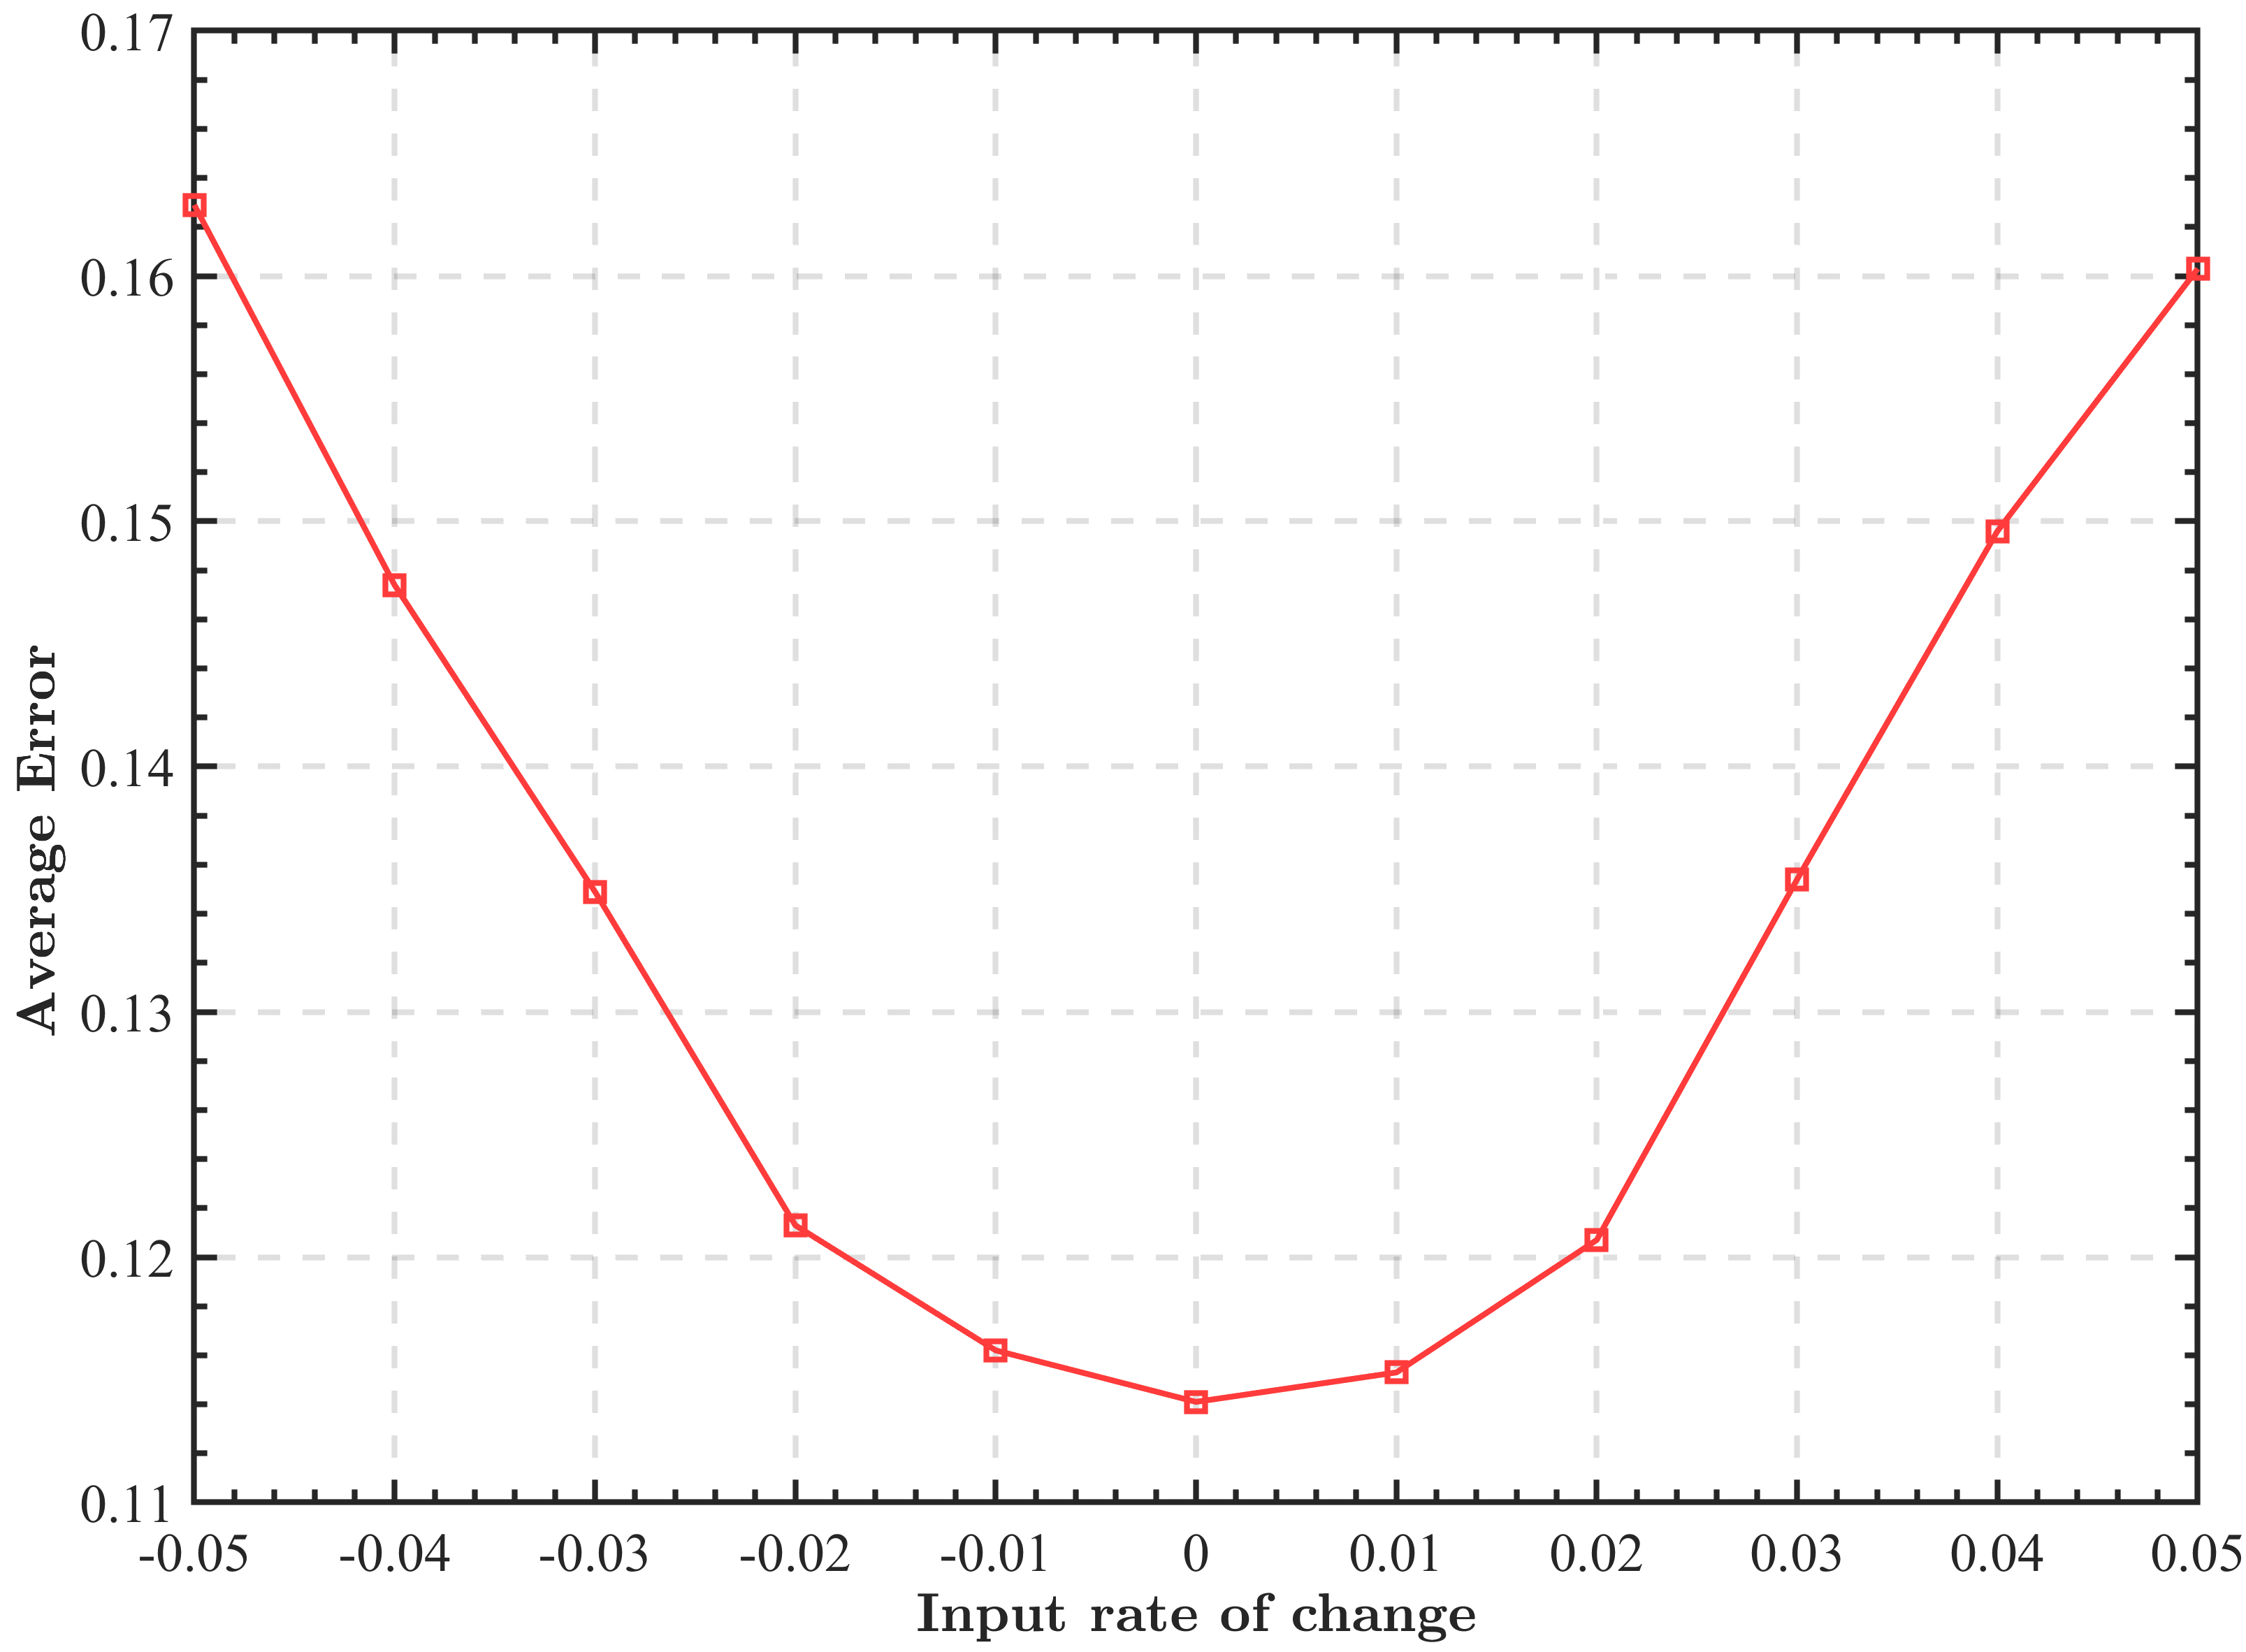
\includegraphics[width=0.31\textwidth]{test_28.png}}			  % 子图1的图片宽度 不能空行
    \subfigure[Monohull Forecast]{				% 图片2
    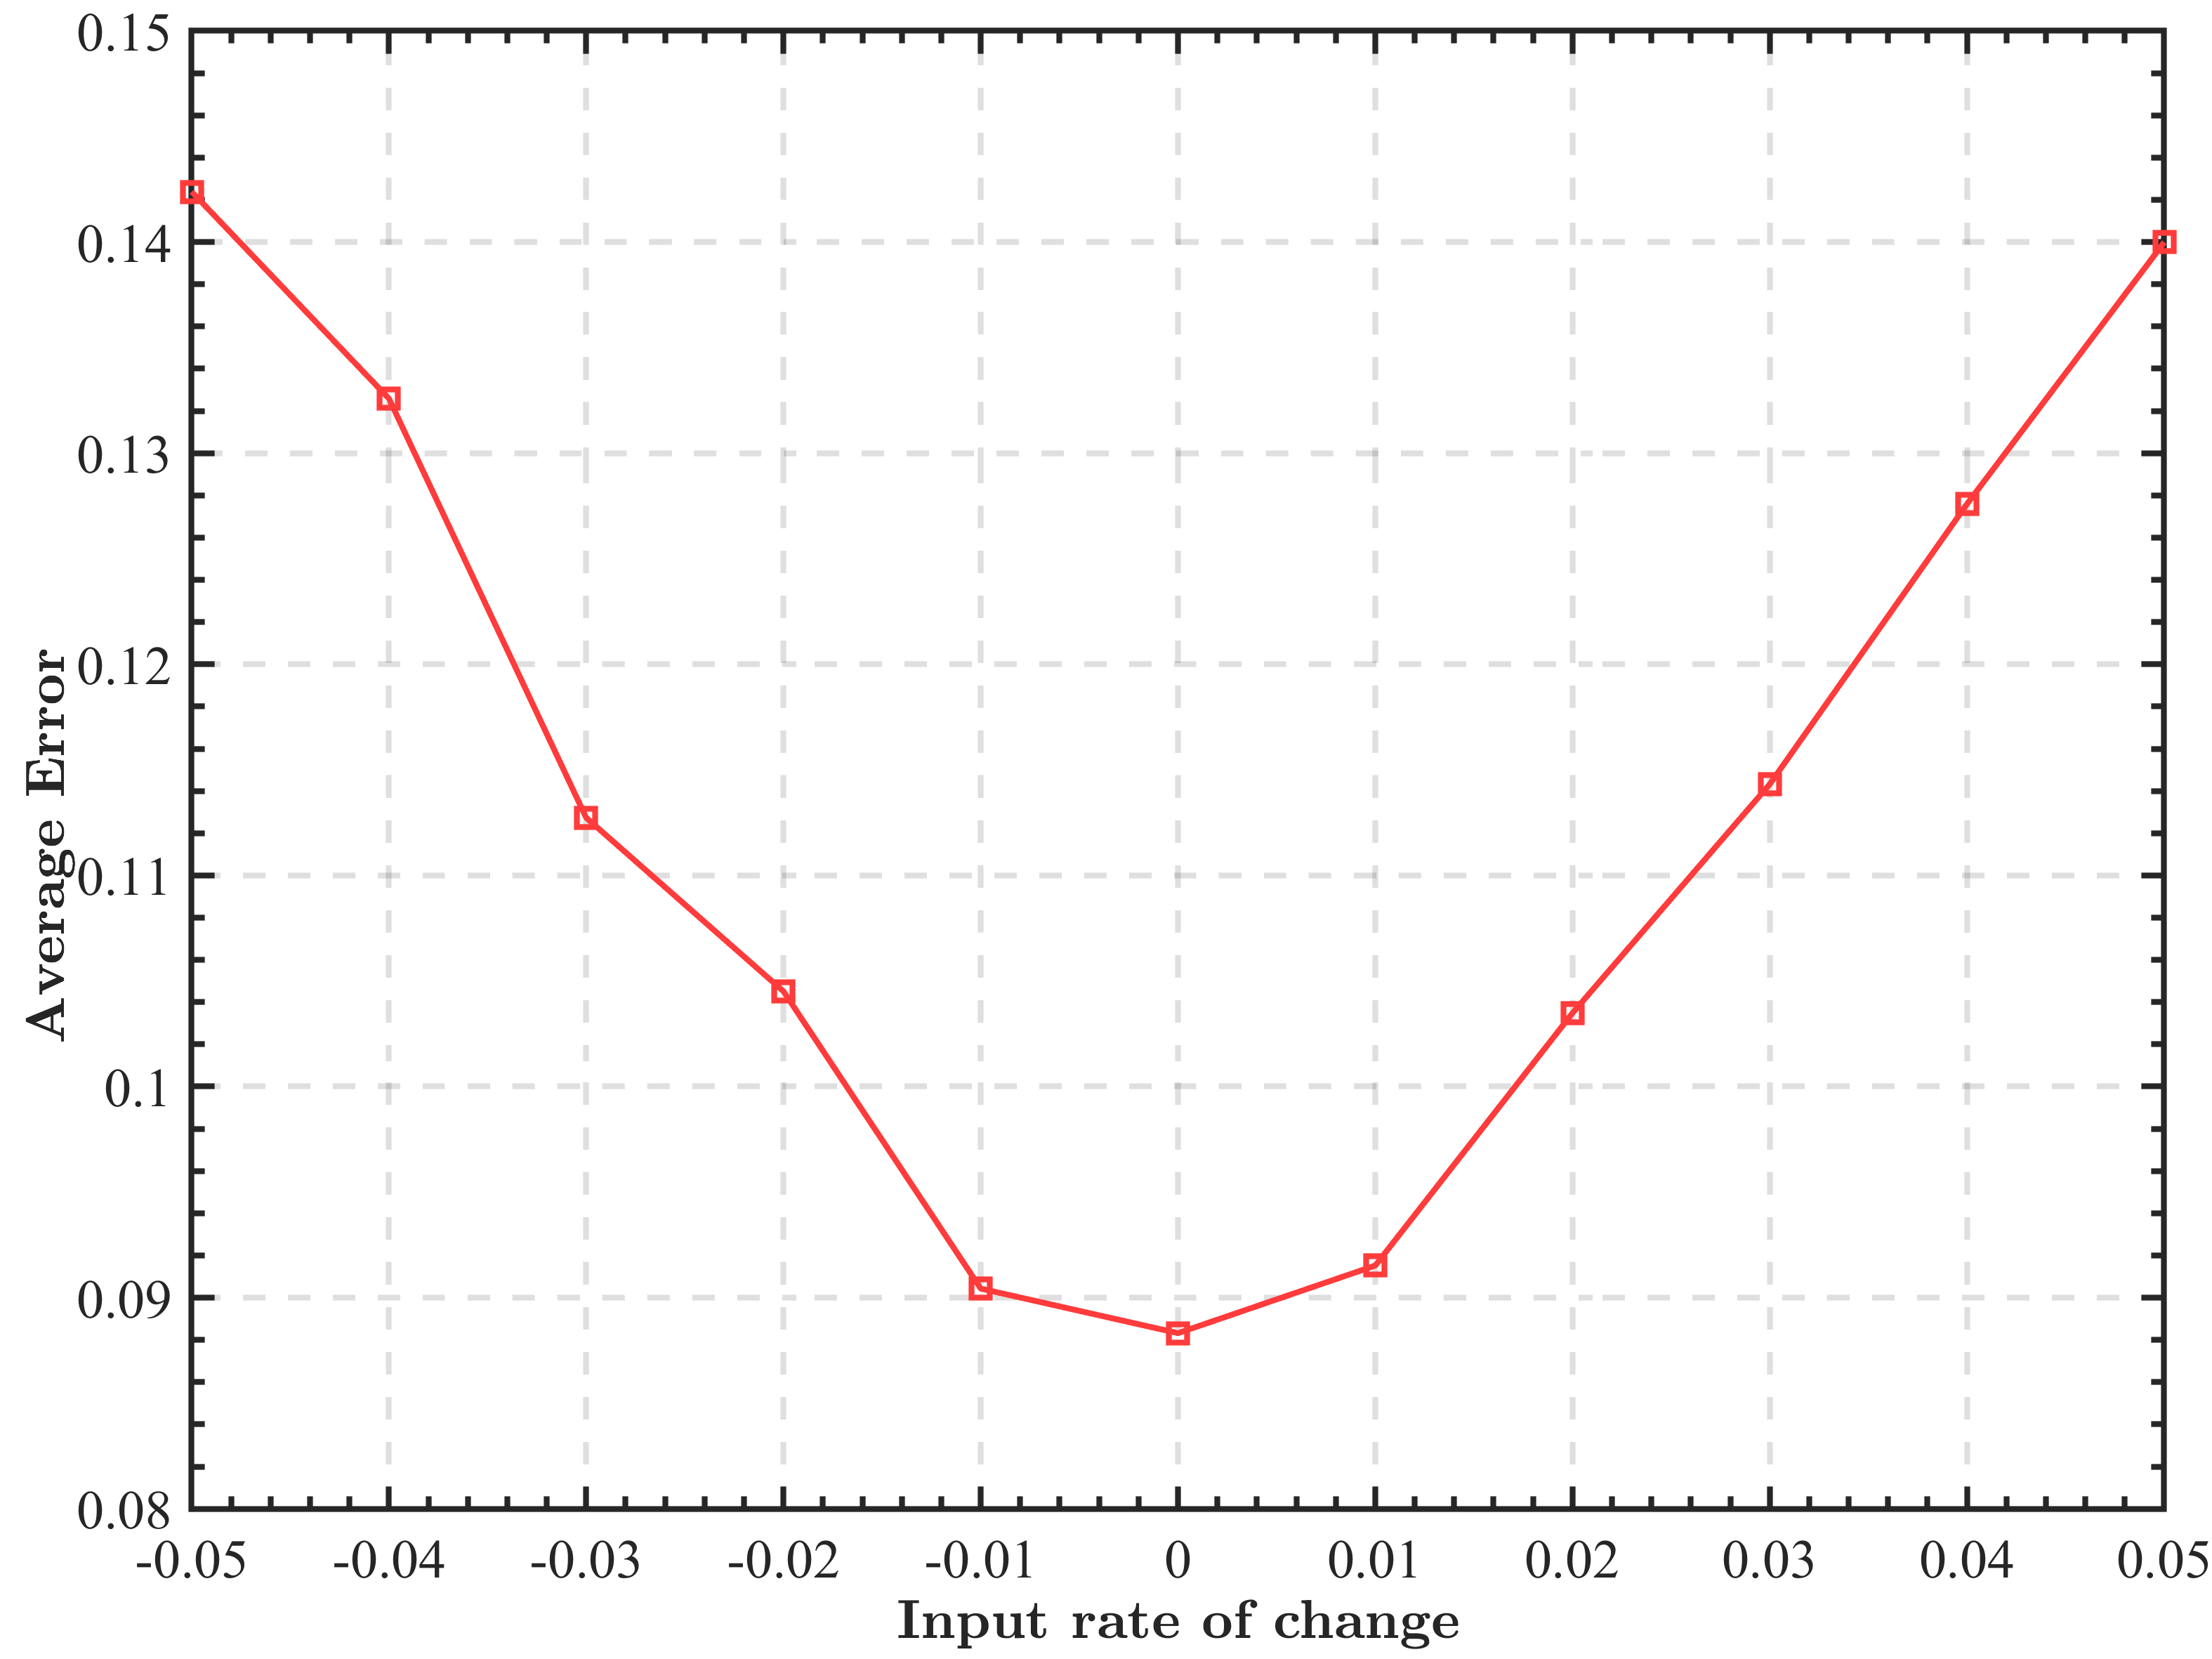
\includegraphics[width=0.31\textwidth]{test_29.png}} 
    \subfigure[Catamaran Forecast]{				% 图片2
    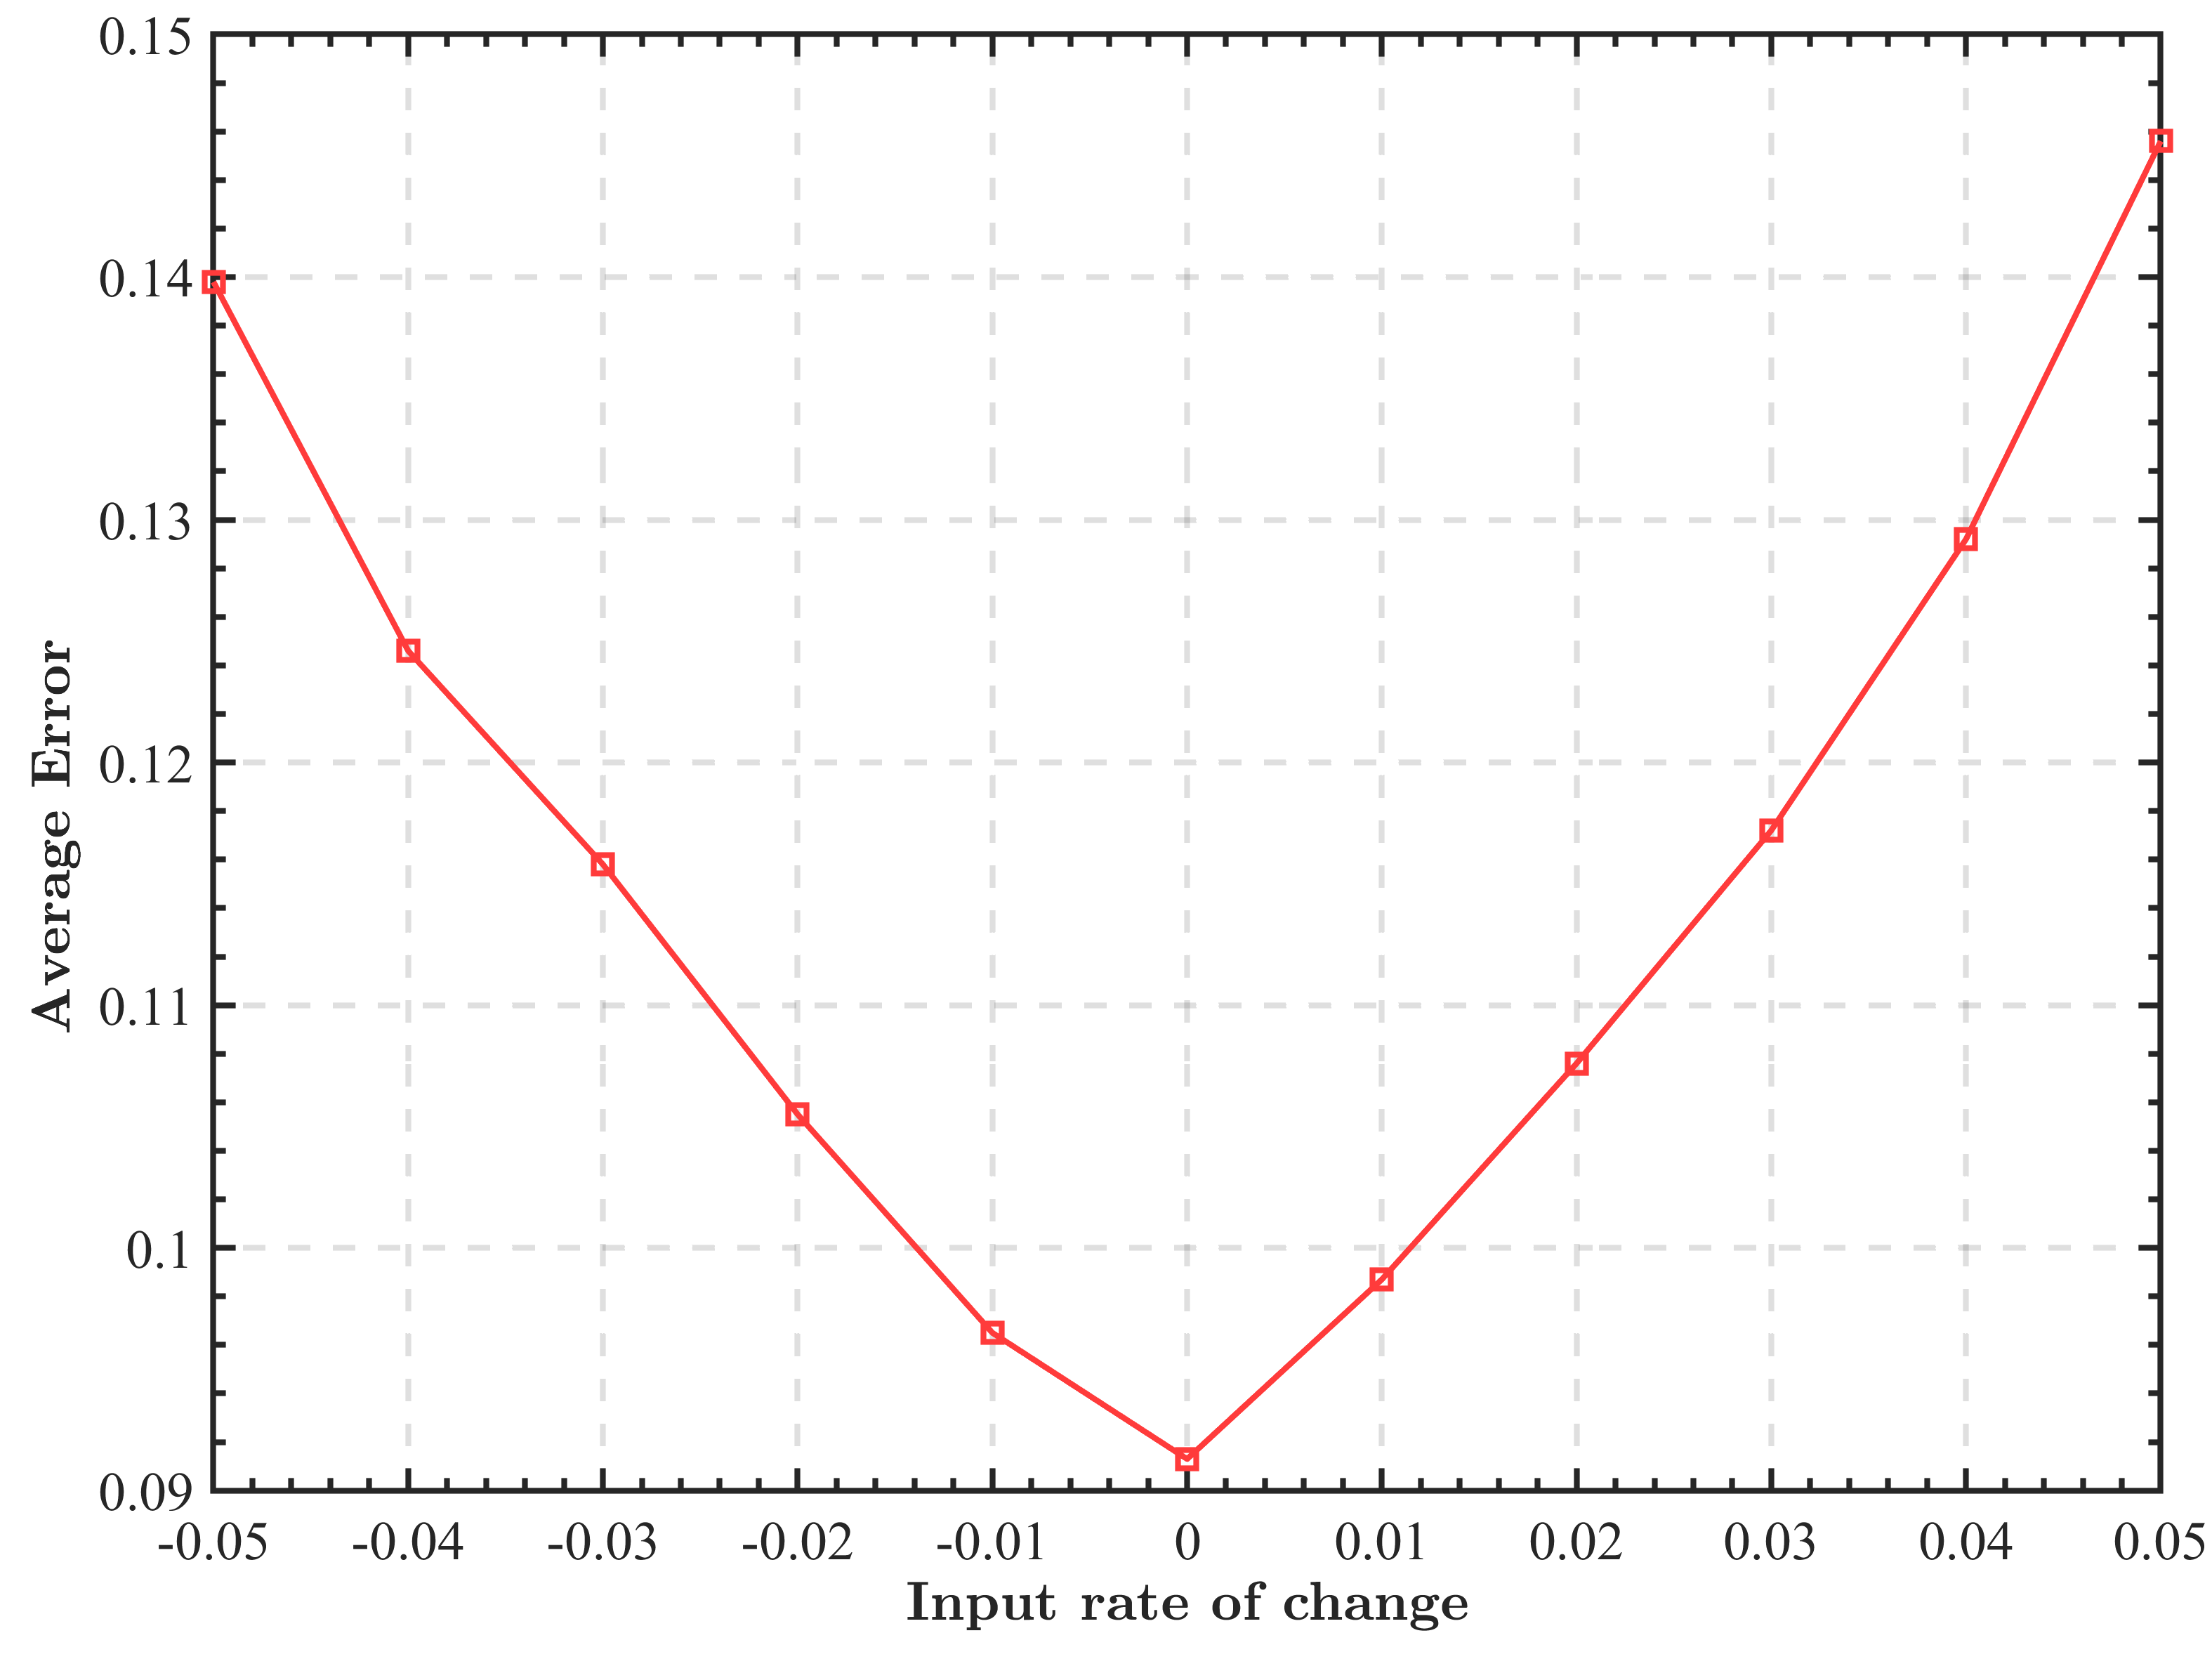
\includegraphics[width=0.31\textwidth]{test_30.png}} 
	\caption{Sensitivity Analysis of Each Neural Network} % 图片标题 
    \vspace{-0.5cm}
\end{figure}

As can be seen in the above figure (a), our fusion model exhibits better immunity to in-terference when the input values change. And from the two figures (b) and (c), we can see that the predicted data of the monohull is more resistant to interference. Although the pre-dicted data of catamaran is less resistant to interference but it does not vary much under the 5\% error band range, and the robustness of the model is better.

\section{Model Evaluation and Further Discussion}
\subsection{Strengths}
Our model offers the following strengths: 
\begin{itemize}
    \setlength{\parsep}{0ex} %段落间距
    \setlength{\topsep}{2ex} %列表到上下文的垂直距离
    \setlength{\itemsep}{1ex} %条目间距
    \item Our model has effectively achieved all the objectives, and it is based on the large data set of 12 parameter indicators of the sailboat, which has high reliability and stability;
    \item The visualization work is done very well by us, such as the research methodolog-ical framework of the article, the prediction effect of three intelligent algorithms and their fusion algorithms, the pie chart of the regional effect of variant sailboats, the chart of the prediction algorithm of sailboat prices in Hong Kong region, etc. Boring data may be able to reflect the law, but not as intuitive as so many images;
    \item We have more innovative and fusion methods, such as RF, the fusion of BP and CNN methods, the method of calculating regional effect indicators based on the change of sailboat ranking and the method of estimating the selling price of sail-boats in Hong Kong based on BP neural network.
\end{itemize}
\subsection{Weaknesses \texorpdfstring{$\&$} FFurther Discussion}
\begin{itemize}
    \setlength{\parsep}{0ex} %段落间距
    \setlength{\topsep}{2ex} %列表到上下文的垂直距离
    \setlength{\itemsep}{1ex} %条目间距
    \item The fusion of multiple models such as random forest may increase the time cost and complexity of the algorithm. In practice, the fused algorithms should be se-lected appropriately to balance the time cost and complexity cost;
    \item Since we did not find the actual selling price of sailboats in Hong Kong, the estimation results using BP neural network may be biased;
    \item The same predictions for used sailboats can be applied to products such as used cars and used houses. It provides guidance for the development of the used economy.
\end{itemize}

\section{Conclusion}
By analyzing the prices of used sailboats with their parameters, the regional effects of prices are also explored and eventually analyzed using Hong Kong, China as a validation for the region. Ultimately we obtained the following main conclusions.
\begin{itemize}
    \setlength{\parsep}{0ex} %段落间距
    \setlength{\topsep}{2ex} %列表到上下文的垂直距离
    \setlength{\itemsep}{1ex} %条目间距
    \item The relationship between regional indicators and the selling price of sailboats\\
    GDP per capita and average temperature are positively cor-related with sailing, in-dicating that people are more enthusiastic about water sports such as sailing when the economic level is higher or when the temperature is higher, which causes an increase in the selling price at that time. Precipitation and unemployment, on the other hand, reduce the sales of sailboats, which results in lower prices.
    \item Sailboats with significant price area effect\\
    The calculation of the change in the ranking of sailing boats allows us to obtain an indicator of the regional effect of sailing boats. After dividing according to this in-dicator, we found that the regional effect is not significant for the following types of boats: Hanse, Dufour, Leopard and Fountaine.
    \item The sales pattern of some sailboats\\
    From the known data, the sales of monohulls are decreasing while the sales of catamarans are increasing. At the same time there will be a clear regional effect for some sailing boats. When buying a sailboat, you should pay attention to the rela-tionship between the regional effect and the price.
\end{itemize}

In conclusion, these findings have greater implications for our study of pricing strate-gies for used sailboats and their regional effects. Also the study for the Hong Kong region can rapidly promote the economic development of the Hong Kong region.

%\begin{center}
%    \LaTeX\\
%    \Huge{\textxswup}\\
%    \normalsize{Word}
%\end{center}

%\input{Memo.tex}
\newpage
% 参考文献,此处以 MLA 引用格式为例
\clearpage   %另起一页继续写。这时,你最好使用“\clearpage” 
\begin{thebibliography}{99}
    \bibitem{1} GLOBAL FOREST WHATCH OF AUSTRALIA \\https://www.globalforestwatch.org/topics/fires/?topic=fires\#footer
	\bibitem{2} HU Teng, LIU Zhanjun, LIU Yang, et al. 3D reconnaissance path planning of multiple UAVs. Journal of Systems Engineering and Electronics, 2019, 41(7): 1551-1559.
	\bibitem{3} BASBOUS B. 2D UAV path planning with radar threatening areas using simulated an-nealing algorithm for event detection. The 2018 International Conference on Artificial Intelligence and Data Processing. Malatya, Turkey: IEEE,2018: 1-7.
	\bibitem{4} WANG W F, WU Y C, ZHANG X. Research of the unit decomposing traversal method based on grid method of the mobile robot. Techniques of Automation and Applications, 2013, 32(11): 34-38.
	\bibitem{5} XU Jian, ZHOU Deyun, HUANG He. Multi UAV path planning based on improved ge-netic algorithm. Aeronautical Computing Technique, 2009, 39(4): 43-46.
\end{thebibliography}
\textbf{}The following codes are written by $Python$, which is to collect the data.
\appendix

%\tcblistof[\section]{mcode}{List of MATLAB code}
\section{First Section}
\begin{matlab}{My 1st Code(Written by MATLAB)}{code:labels}
% a comment
clear all, clc
% a comment
x = [1.00; 1.00; 1.00];
beta0 = [1 1 1];
modelfun = 'y ~ k*x^2+b'
mdl = fitnlm(tb,modelfun,beta0)
% a comment
plotResiduals(md1,'fitt111111111111111ed')
%this is a loooooooooooooo ooooooooooooooooooooooooooo oooooooooooooooooog




%1
\end{matlab}
\begin{matlab}{My 2st Code}{code:llabel}
disp('hello')
\end{matlab}
\begin{matlab}{My 2st Code}{code:labell}
    disp('hello')
\end{matlab}
\section{ccODE}

\begin{align}
\end{align}
\end{document}  % 结束